
\documentclass{article} % For LaTeX2e

% DECISION: (contract 7.2-7.3) venue order (TMLR, then J2C) and whether A goes to arXiv
% before B is submitted are group decisions; this draft keeps the TMLR style.
% ---------------------------------------------------------------------------
% TMLR submission (style files from github.com/JmlrOrg/tmlr-style-file).
% Compile:  pdflatex main && bibtex main && pdflatex main && pdflatex main
%
% Anonymized for double-blind review: with no option, tmlr.sty prints
% "Anonymous authors" and the "Under review" header, so no author
% name/affiliation/email may appear in this file. Use \usepackage[accepted]{tmlr}
% only for the camera-ready version, [preprint] for arXiv.
% ---------------------------------------------------------------------------

\ifdefined\iclrversion
  \usepackage{iclr2027_conference,times}
\else
  \usepackage{tmlr}
\fi
% \moveblock{name}{...} prints a block in place for TMLR and stores it for ICLR,
% where \placeblock{name} prints it in the appendix: one source for both venues.
\newif\ificlr
\ifdefined\iclrversion\iclrtrue\fi
\makeatletter
\newcommand{\moveblock}[2]{\@namedef{moved@#1}{#2}\ificlr\else#2\fi}
\newcommand{\placeblock}[1]{\ificlr\@nameuse{moved@#1}\fi}
\makeatother
% Display breaks for the narrower ICLR column; empty (\iclrqbr: \qquad) for TMLR.
% \iclrbr breaks at a relation, \iclrbrq breaks with an indent, \iclrqbr breaks
% where TMLR has \qquad, and \iclrstart...\iclrend make a single display breakable;
% \iclrallow allows a line break inside a file path.
\ificlr
  \newcommand{\iclrbr}{\\&}\newcommand{\iclrbrq}{\\&\qquad}\newcommand{\iclrqbr}{\\&}
  \newcommand{\iclrstart}{\begin{aligned}&}\newcommand{\iclrend}{\end{aligned}}
  \newcommand{\iclrallow}{\allowbreak}
\else
  \newcommand{\iclrbr}{}\newcommand{\iclrbrq}{}\newcommand{\iclrqbr}{\qquad}
  \newcommand{\iclrstart}{}\newcommand{\iclrend}{}\newcommand{\iclrallow}{}
\fi
\usepackage{amsmath,amssymb,amsthm}
\usepackage{thmtools,thm-restate} % main-text results restated verbatim before their proofs
\usepackage{graphicx}
\usepackage{booktabs}
\usepackage{caption}
\usepackage{subcaption}
\usepackage{xcolor}
\usepackage[colorlinks=true,linkcolor=blue,citecolor=blue,urlcolor=blue]{hyperref}
\usepackage{placeins} % \FloatBarrier keeps figures/tables from drifting past a subsection
\usepackage{enumitem} % lettered sub-claims inside lemma statements
\usepackage{standalone} % \input of the standalone TikZ figures in figures/tikz/
\usepackage{tikz}
\usetikzlibrary{positioning, arrows.meta, shapes.geometric, shapes.misc, fit, backgrounds, calc}
% OpenTikZ palette (Okabe-Ito, as in scripts/figstyle.py) for the TikZ figures
\definecolor{otblue}{HTML}{0072B2}
\definecolor{otorange}{HTML}{E69F00}
\definecolor{otteal}{HTML}{009E73}
\definecolor{otpurple}{HTML}{CC79A7}
\definecolor{otgray}{HTML}{5A5A5A}
\definecolor{otverm}{HTML}{D55E00}
% result numbers inside the TikZ figures: a live \ref here, a fallback when standalone
\newcommand{\resref}[2]{\ref{#1}}

\graphicspath{{figures/}}

% --- theorem environments -------------------------------------------------
% One counter per section shared by all results (Theorem 4.1, Lemma B.2, ...).
\theoremstyle{plain}
\newtheorem{theorem}{Theorem}[section]
\newtheorem{proposition}[theorem]{Proposition}
\newtheorem{lemma}[theorem]{Lemma}
\newtheorem{corollary}[theorem]{Corollary}
\theoremstyle{definition}
\newtheorem{assumption}{Assumption}
\theoremstyle{remark}
\newtheorem{remark}[theorem]{Remark}
\newenvironment{proofsketch}{\begin{proof}[Proof sketch]}{\end{proof}}
% The pointer [Proof: Appendix X] is printed in the main text only, not in restatements.
\newif\ifproofpointer \proofpointertrue
% Unique hyperref anchors: restatements in the appendix get their own prefix.
\makeatletter
\@for\thm@env:=theorem,proposition,lemma,corollary,remark\do{%
  \expandafter\def\csname theH\thm@env\endcsname{\ifproofpointer\else apx.\fi\thetheorem}}
\makeatother

% --- shorthands: paper/math_commands.tex ------------------------------------
%%%%% MATH DEFINITIONS, shared by the body and Appendix A %%%%%
% Read by main.tex with %%%%% MATH DEFINITIONS, shared by the body and Appendix A %%%%%
% Read by main.tex with %%%%% MATH DEFINITIONS, shared by the body and Appendix A %%%%%
% Read by main.tex with \input{math_commands}. Proofs use the shorthands at the end,
% so that a display is a line of mathematics and not a line of \frac's.

% --- sets and operators ---------------------------------------------------
\newcommand{\R}{\mathbb{R}}
\newcommand{\E}{\mathbb{E}}
\newcommand{\Var}{\operatorname{Var}}
\newcommand{\Cov}{\operatorname{Cov}}
\newcommand{\tr}{\operatorname{tr}}
\newcommand{\N}{\mathcal{N}}
\newcommand{\D}{\mathcal{D}}
\newcommand{\dist}{\operatorname{dist}}
\newcommand{\supp}{\operatorname{supp}}
\newcommand{\law}{\mathrm{Law}}
\newcommand{\ind}{\mathbf{1}}
\newcommand{\eps}{\varepsilon}

% --- objects of the paper -------------------------------------------------
\newcommand{\Sigmapost}{\Sigma_{\mathrm{post}}}
\newcommand{\Xhat}{\widehat{\Sigma}_X}
\newcommand{\rhohat}{\widehat{\rho}}
\newcommand{\vstar}{v_h^\star}
\newcommand{\vstarz}{v_0^\star}
\newcommand{\Covh}{\operatorname{Cov}_h}
% nearest training atoms of a point, and the open probability simplex
\newcommand{\nn}{\operatorname{nn}}
\newcommand{\Ppos}{\mathcal{P}_N^{+}}

% --- shorthands for the proofs --------------------------------------------
% label weight and kernel weight of atom #1 at bandwidth h
\newcommand{\pih}[1]{p_{#1}^{(h)}}
\newcommand{\wih}[1]{w_{#1}^{(h)}}
% label kernel K_h(y - y^i)
\newcommand{\KK}[1]{K_h(y-y^{#1})}
% per-atom collapsed field (a_i - x)/(1 - t)
\newcommand{\fat}[1]{\frac{a_{#1}-x}{1-t}}
% source density at the point that reaches x from atom #1
\newcommand{\src}[1]{\pi_0\!\Big(\frac{x-ta_{#1}}{1-t}\Big)}

% --- pointer from a statement in the body to its proof --------------------
% (main.tex sets \proofpointerfalse in the appendix, so restatements omit it)
\providecommand{\ifproofpointer}{\iftrue}
\newcommand{\proofin}[1]{\ifproofpointer\hfill\textnormal{\footnotesize[Proof: Appendix~\ref{#1}]}\fi}
. Proofs use the shorthands at the end,
% so that a display is a line of mathematics and not a line of \frac's.

% --- sets and operators ---------------------------------------------------
\newcommand{\R}{\mathbb{R}}
\newcommand{\E}{\mathbb{E}}
\newcommand{\Var}{\operatorname{Var}}
\newcommand{\Cov}{\operatorname{Cov}}
\newcommand{\tr}{\operatorname{tr}}
\newcommand{\N}{\mathcal{N}}
\newcommand{\D}{\mathcal{D}}
\newcommand{\dist}{\operatorname{dist}}
\newcommand{\supp}{\operatorname{supp}}
\newcommand{\law}{\mathrm{Law}}
\newcommand{\ind}{\mathbf{1}}
\newcommand{\eps}{\varepsilon}

% --- objects of the paper -------------------------------------------------
\newcommand{\Sigmapost}{\Sigma_{\mathrm{post}}}
\newcommand{\Xhat}{\widehat{\Sigma}_X}
\newcommand{\rhohat}{\widehat{\rho}}
\newcommand{\vstar}{v_h^\star}
\newcommand{\vstarz}{v_0^\star}
\newcommand{\Covh}{\operatorname{Cov}_h}
% nearest training atoms of a point, and the open probability simplex
\newcommand{\nn}{\operatorname{nn}}
\newcommand{\Ppos}{\mathcal{P}_N^{+}}

% --- shorthands for the proofs --------------------------------------------
% label weight and kernel weight of atom #1 at bandwidth h
\newcommand{\pih}[1]{p_{#1}^{(h)}}
\newcommand{\wih}[1]{w_{#1}^{(h)}}
% label kernel K_h(y - y^i)
\newcommand{\KK}[1]{K_h(y-y^{#1})}
% per-atom collapsed field (a_i - x)/(1 - t)
\newcommand{\fat}[1]{\frac{a_{#1}-x}{1-t}}
% source density at the point that reaches x from atom #1
\newcommand{\src}[1]{\pi_0\!\Big(\frac{x-ta_{#1}}{1-t}\Big)}

% --- pointer from a statement in the body to its proof --------------------
% (main.tex sets \proofpointerfalse in the appendix, so restatements omit it)
\providecommand{\ifproofpointer}{\iftrue}
\newcommand{\proofin}[1]{\ifproofpointer\hfill\textnormal{\footnotesize[Proof: Appendix~\ref{#1}]}\fi}
. Proofs use the shorthands at the end,
% so that a display is a line of mathematics and not a line of \frac's.

% --- sets and operators ---------------------------------------------------
\newcommand{\R}{\mathbb{R}}
\newcommand{\E}{\mathbb{E}}
\newcommand{\Var}{\operatorname{Var}}
\newcommand{\Cov}{\operatorname{Cov}}
\newcommand{\tr}{\operatorname{tr}}
\newcommand{\N}{\mathcal{N}}
\newcommand{\D}{\mathcal{D}}
\newcommand{\dist}{\operatorname{dist}}
\newcommand{\supp}{\operatorname{supp}}
\newcommand{\law}{\mathrm{Law}}
\newcommand{\ind}{\mathbf{1}}
\newcommand{\eps}{\varepsilon}

% --- objects of the paper -------------------------------------------------
\newcommand{\Sigmapost}{\Sigma_{\mathrm{post}}}
\newcommand{\Xhat}{\widehat{\Sigma}_X}
\newcommand{\rhohat}{\widehat{\rho}}
\newcommand{\vstar}{v_h^\star}
\newcommand{\vstarz}{v_0^\star}
\newcommand{\Covh}{\operatorname{Cov}_h}
% nearest training atoms of a point, and the open probability simplex
\newcommand{\nn}{\operatorname{nn}}
\newcommand{\Ppos}{\mathcal{P}_N^{+}}

% --- shorthands for the proofs --------------------------------------------
% label weight and kernel weight of atom #1 at bandwidth h
\newcommand{\pih}[1]{p_{#1}^{(h)}}
\newcommand{\wih}[1]{w_{#1}^{(h)}}
% label kernel K_h(y - y^i)
\newcommand{\KK}[1]{K_h(y-y^{#1})}
% per-atom collapsed field (a_i - x)/(1 - t)
\newcommand{\fat}[1]{\frac{a_{#1}-x}{1-t}}
% source density at the point that reaches x from atom #1
\newcommand{\src}[1]{\pi_0\!\Big(\frac{x-ta_{#1}}{1-t}\Big)}

% --- pointer from a statement in the body to its proof --------------------
% (main.tex sets \proofpointerfalse in the appendix, so restatements omit it)
\providecommand{\ifproofpointer}{\iftrue}
\newcommand{\proofin}[1]{\ifproofpointer\hfill\textnormal{\footnotesize[Proof: Appendix~\ref{#1}]}\fi}


\title{Which Interventions Keep a Conditional Flow\\
on Its Training Set?}

% Authors must not appear in the submitted version; tmlr.sty ignores \author
% unless the [accepted] or [preprint] option is given. Fill in names only then.
\author{Anonymous authors}
\newcommand{\openreview}{\url{https://openreview.net/forum?id=XXXX}}

\begin{document}
\maketitle
\raggedbottom

% DECISION: (contract 7.1) the final headline of A is a group decision. This draft keeps the
% current one (the number and signs of the combined exact fields decide the support); the
% AND/class-label proposition is not added (contract 7.4, section 5).
\begin{abstract}
Conditional flow-matching samplers rarely integrate the field that their objective targets.
Labels are noised during training, a network that resolves labels coarsely averages the field
over nearby labels, and sampling adds classifier-free guidance, guidance schedules, negative
prompts, or the summed guidance terms of compositional generation. Some of these changes are used
to reduce the replication of training data. We ask which of them can move the endpoints of the
exact empirical field, the population minimiser for a fixed training set, off the training
examples. The answer depends on how many exact fields are combined, and with which signs. Label
noise only reweights the training examples, with weights computable from the labels. Positive
mixtures of exact fields with strictly positive priors, every fixed combination of two such
fields, which includes negative prompting by substitution, and guidance with a nonnegative bounded
schedule of bounded variation end on a training example from almost every initial point. For
guidance, the analogous statement was known for the stochastic sampler, and for a fixed strength
every trajectory of the flow was known to converge, possibly to a point that is not a training
example. Three fields can blend training examples. The conjunction of compositional generation
reaches a blend with positive probability. For two examples with prior log-odds $\pm2B$ this
happens exactly when the guidance strength exceeds $1/\sinh^2B$, and in any dimension the
eigenvalue signs of a signed posterior covariance decide it. At a tie of two examples, a blend
requires subtracting a field that is less decided between them than the fields added. The blend
basin lies in a layer of width $(1-t)^2$ around the tie. Standard velocity networks miss it, while
networks given a coordinate at that scale, centred at the tie, can match its exact probability.
For an audit of replication, the results separate the sampler settings that at the exact optimum
can only return training examples from the composition of conditions, which can blend them.
\end{abstract}

% ==========================================================================
\section{Introduction}
\label{sec:intro}
% Overview schematic first, so that it floats to the top of page 2; the hero figure follows.
\suppressfloats[t]% no top floats on the title page
\begin{figure}[t]
\centering
\IfFileExists{figures/tikz/overview.tex}{\documentclass[border=3pt]{standalone}
% Overview schematic of paper A (figure fig:overview), drawn as a CV architecture figure:
% coloured blocks with a depth face (block style borrowed from PlotNeuralNet), arrows that mean
% "sampling from pi_0 ends at", parameters under the blocks and a legend in the lower-left corner.
% Compiles on its own; main.tex \input's it through the standalone package (preamble dropped), so
% everything it needs beyond tikz and the libraries below is defined inside the document body.
% Natural width is about 15.6 cm: it fits \textwidth without scaling.

% --- packages (mirrored in main.tex) ---
\usepackage{amsmath,amssymb}
\usepackage{tikz}
\usetikzlibrary{positioning, arrows.meta, fit, backgrounds, calc}

% result numbers: printed as fallbacks here, as \ref in main.tex
\providecommand{\resref}[2]{#2}

\begin{document}
% Okabe-Ito, same values as scripts/figstyle.py: blue = exact field, black = training example,
% vermillion = blend (the roles of the data figures).
\definecolor{ovblue}{HTML}{0072B2}
\definecolor{ovsky}{HTML}{56B4E9}
\definecolor{ovverm}{HTML}{D55E00}
\definecolor{ovgray}{HTML}{5A5A5A}
% depth face of a block: top and right parallelograms, as in PlotNeuralNet's Box
\providecommand{\ovfaces}[2]{%
  \draw[#2!65!black, line width=0.5pt, fill=#2!38, line join=round]
    (#1.north west) -- ++(0.2,0.15) -- ($(#1.north east)+(0.2,0.15)$) -- (#1.north east) -- cycle;
  \draw[#2!65!black, line width=0.5pt, fill=#2!55, line join=round]
    (#1.north east) -- ++(0.2,0.15) -- ($(#1.south east)+(0.2,0.15)$) -- (#1.south east) -- cycle;}
% a training example and a blend, as drawn in the data figures
\providecommand{\ovatom}[1]{\fill[black] ($(#1)+(0,0.085)$) -- ++(-0.085,-0.15) -- ++(0.17,0) -- cycle;}
\providecommand{\ovblend}[1]{\fill[ovverm, draw=white, line width=0.3pt]
  ($(#1)+(0,0.085)$) -- ++(0.085,-0.085) -- ++(-0.085,-0.085) -- ++(-0.085,0.085) -- cycle;}

\begin{tikzpicture}[
    font=\sffamily\footnotesize,
    >={Stealth[length=2mm]},
    blk/.style={draw=#1!65!black, fill=#1!14, line width=0.5pt, align=center,
      minimum height=1.25cm, inner sep=3pt},
    slab/.style={draw=ovblue!55!black, fill=ovsky!18, line width=0.45pt, align=center,
      text width=2.0cm, minimum height=0.62cm, inner sep=1.5pt, font=\sffamily\scriptsize},
    term/.style={draw=#1, fill=white, line width=0.9pt, rounded corners=6pt, align=center,
      minimum width=2.5cm, minimum height=1.25cm, inner sep=3pt},
    param/.style={font=\sffamily\scriptsize, text=ovgray, align=center},
    lane/.style={draw=#1, dashed, line width=0.5pt, rounded corners=4pt, inner sep=5pt},
    lanetitle/.style={font=\sffamily\scriptsize\bfseries, text=#1, anchor=south west, inner sep=1pt},
    flow/.style={->, draw=ovgray, line width=0.8pt},
  ]

  % ---- input and the exact field ------------------------------------------------------------
  \node[blk=ovgray, minimum width=2.2cm, text depth=0.55cm] (data) at (0,0)
    {finite training set};
  \ovfaces{data}{ovgray}
  \foreach \x/\s in {-0.65/1, -0.2/2, 0.65/N} {
    \ovatom{$(data.center)+(\x,-0.12)$}
    \node[font=\sffamily\tiny, text=ovgray] at ($(data.center)+(\x,-0.42)$) {$y^{\s}$};
  }
  \node[font=\sffamily\tiny, text=ovgray] at ($(data.center)+(0.22,-0.17)$) {$\cdots$};
  \node[param, below=0.12cm of data] {$N$ examples $x^i$\\with labels $y^i$};

  \node[blk=ovblue, minimum width=2.4cm, right=0.6cm of data] (field)
    {exact conditional\\field $v^\star_y$};
  \ovfaces{field}{ovblue}
  \node[param, below=0.12cm of field] {minimiser of the\\flow-matching loss};
  \draw[flow] (data.east) -- (field.west);

  % ---- top lane: one intervention at a time ---------------------------------------------------
  \node[slab, anchor=south west] (noise) at ($(field.east)+(1.0,0.95)$) {label noise, $h>0$};
  \node[slab, right=0.12cm of noise] (avg1) {label averaging\\at \mbox{$h>0$}};
  \node[slab, below=0.12cm of noise] (cfg) {guidance, $w\ge0$};
  \node[slab, right=0.12cm of cfg] (sched) {bounded\\schedule $w(t)$};
  \node[lane=ovblue, fit=(noise)(avg1)(cfg)(sched)] (top) {};
  \node[lanetitle=ovblue!80!black] at (top.north west) {any one intervention};
  \node[param, below=0.08cm of top]
    {Thm.~\resref{thm:endpoint}{3.4}, Thm.~\resref{thm:posmix}{4.1},
     Prop.~\resref{prop:cfgatom}{4.4}, Thm.~\resref{thm:schedule}{4.6}};

  \node[term=black, right=0.7cm of top] (atom) {ends on a\\training example\\[0.42cm]};
  \foreach \x in {-0.35, 0, 0.35} {\ovatom{$(atom.center)+(\x,-0.3)$}}
  \node[param, below=0.12cm of atom] {almost surely;\\only the weights change};

  % ---- bottom lane: composition, a label average followed by guidance --------------------------
  \node[blk=ovblue, minimum width=1.85cm, anchor=north west] (avg2)
    at ($(top.south west)+(0.0,-1.15)$) {label\\averaging};
  \ovfaces{avg2}{ovblue}
  \node[param, below=0.12cm of avg2] {averages the fields\\of several labels};
  \node[blk=ovblue, minimum width=1.85cm, right=0.55cm of avg2] (guid) {guidance\\at strength $w$};
  \ovfaces{guid}{ovblue}
  \node[param, below=0.12cm of guid, text=ovverm!85!black, font=\sffamily\footnotesize]
    {$w>w_c=\dfrac{1}{\sinh^2 B}$};
  \draw[flow] (avg2.east) -- (guid.west);
  \coordinate (guidback) at ($(guid.north east)+(0.2,0.15)$);
  \begin{scope}[on background layer]
    \node[lane=ovverm, fit=(avg2)(guid)(guidback)] (bot) {};
  \end{scope}
  \node[lanetitle=ovverm!85!black] at (bot.north west) {composition: three exact fields};

  \node[term=ovverm, anchor=west] (blend) at (atom.west |- bot.east)
    {ends on a blend of\\training examples\\[0.42cm]};
  \ovatom{$(blend.center)+(-0.42,-0.3)$}
  \ovblend{$(blend.center)+(0,-0.3)$}
  \ovatom{$(blend.center)+(0.42,-0.3)$}
  \node[param, below=0.12cm of blend] {with positive probability\\(Thm.~\resref{thm:composition}{4.8})};

  % ---- arrows: "sampling from pi_0 under this field ends at" ---------------------------------
  \coordinate (fork) at ($(field.east)+(0.5,0)$);
  \draw[draw=ovgray, line width=0.8pt] (field.east) -- (fork);
  \draw[flow] (fork) |- (top.west);
  \draw[flow] (fork) |- (bot.west);
  \draw[flow] (top.east) -- (atom.west);
  \draw[flow, draw=ovverm] (bot.east) -- (blend.west);

  % ---- legend, lower-left corner ---------------------------------------------------------------
  \begin{scope}[shift={($(data.south west)+(0.0,-1.65)$)}, font=\sffamily\scriptsize]
    \fill[ovblue!14, draw=ovblue!65!black, line width=0.5pt] (0,0) rectangle (0.32,0.2);
    \node[anchor=west] at (0.4,0.1) {field built from exact fields};
    \ovatom{0.16,-0.27}
    \node[anchor=west] at (0.4,-0.3) {training example};
    \ovblend{0.16,-0.67}
    \node[anchor=west] at (0.4,-0.7) {blend, e.g.\ the midpoint $\tfrac12(x^i+x^j)$};
    \draw[flow] (0,-1.1) -- (0.32,-1.1);
    \node[anchor=west] at (0.4,-1.1) {sampling from $\pi_0$ ends at};
    \node[draw=ovgray!40, rounded corners=2pt, inner sep=3pt, fit={(-0.05,0.28)(4.6,-1.25)}] {};
  \end{scope}
\end{tikzpicture}
\end{document}
}{\fbox{overview schematic pending}}
\caption{Overview. A finite training set $\{(x^i,y^i)\}_{i=1}^N$ and its labels define the exact
conditional field $\vstar$, the population minimiser of the flow-matching objective. Each
intervention studied here replaces $\vstar$ by another field built from exact fields. Label noise
(Theorem~\ref{thm:endpoint}), label averaging (Theorem~\ref{thm:posmix}), guidance with a fixed
strength (Proposition~\ref{prop:cfgatom}) and guidance schedules (Theorem~\ref{thm:schedule}) all
end on training images from almost every initial point; only the weights of the images change.
Composition, guidance applied to the label-averaged field, combines three fields and can end on a
blend of training images, for two images with prior log-odds $\pm2B$ exactly when the guidance
strength exceeds $w_c=1/\sinh^2B$ (Theorem~\ref{thm:composition}).}
\label{fig:overview}
\end{figure}

\begin{figure}[t]
\centering
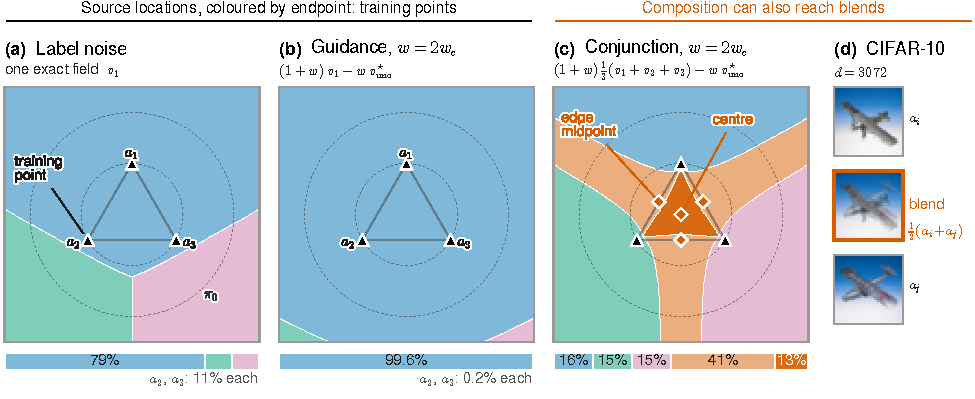
\includegraphics[width=\textwidth]{fig_unrolled_exact.pdf}
\caption{Where each source ends, on a triangle of training points $a_1,a_2,a_3$
(Section~\ref{sec:intervention-tests}, $B=2$; $v_k$ is the exact field of the condition favouring
$a_k$). Each pixel is an initial point $x_0$, coloured by the endpoint of its exact trajectory: a
training point (blue, green, purple) or a blend (vermillion: the centre, dark; an edge midpoint,
light). Circles: one and two standard deviations of $\pi_0$. Bars: the endpoint law under $\pi_0$
($32768$ sources). (a) One field ends on the training points with the label weights of
Theorem~\ref{thm:endpoint}. (b) Guidance with $w=2w_c$ puts almost all the mass at $a_1$, still on
training points (Proposition~\ref{prop:cfgatom}). (c) The same guidance applied to the average of
the three conditional fields, the conjunction, ends $13\%$ of the mass at the centre
(Theorem~\ref{thm:spectral}) and $41\%$ at the edge midpoints, which attract for $w>1.37\,w_c$
(Proposition~\ref{prop:twoatom}(c) at an edge). (d) Two CIFAR-10 training images and their
midpoint, which the exact conjunction of their two conditions reaches for $w>w_c$
(Appendix~\ref{app:cifar-composition}).}
\label{fig:unrolled}
\end{figure}

Flow matching and stochastic-interpolant models
\citep{lipman2023flow,albergo2023building,liu2023rectified,albergo2023stochastic}
regress a velocity field on a path from noise to data. Against the \emph{empirical} law of a fixed
training set the population minimiser is explicit, and its flow returns training examples
\citep{gu2023memorization,biroli2023diffusion,gao2024flow,bertrand2025closed}. A trained network
approximates this exact field, so the exact field says what the objective asks the network to do.
Practical conditional samplers do not integrate it as it is. Labels are noised during
training~\citep{ho2022cascaded}. A network that resolves labels only coarsely averages the field
over nearby labels. Sampling adds classifier-free guidance~\citep{ho2022classifier}, often with a
strength that varies in time~\citep{kynkaanniemi2024interval} or is withheld or reversed early to
reduce memorisation~\citep{jain2025attraction}. Compositional generation adds the guidance terms
of several conditions~\citep{liu2022composable}. Randomising the conditioning reduces copying in
trained text-to-image models~\citep{somepalli2023copying}.

We ask which of these modifications can, alone or combined with another, move the endpoints of
the exact field off the training set. Two groups need the answer. A practitioner who uses label
noise, guidance schedules or negative prompts against copying needs to know whether the knob
changes what the model is asked to produce, or whether any reduction comes only from the error of
the learned field and may disappear with a closer fit. An auditor needs to know which sampler
settings can return a training record at the exact optimum, and which record. The answer depends
on how many exact fields are combined, and with which signs (Figure~\ref{fig:overview},
Table~\ref{tab:interventions}). Combinations of two fields only reweight the training examples.
Three fields can blend them, and at a tie of two examples only with a specific sign pattern.

\paragraph{Contributions.}
\begin{enumerate}[leftmargin=1.5em,itemsep=1pt]
\item \emph{The label-noise reference} (Section~\ref{sec:theory}). With Gaussian label noise of
  bandwidth $h>0$ the exact flow returns the training example $x^i$ with probability
  $p_i^{(h)}(y)$, a Nadaraya--Watson weight computable from the labels
  (Theorem~\ref{thm:endpoint}). Closely related identities are known
  (Section~\ref{sec:related}). We use this law as the starting point of every later result, and
  its variance as a parameter-free reference for trained networks
  (Section~\ref{sec:intervention-tests}).
\item \emph{Two fields only reweight the training examples}
  (Sections~\ref{sec:posmix}--\ref{sec:guidance}). Positive mixtures of prior-indexed exact fields
  with strictly positive priors, which include label averaging, end on a training example from
  almost every initial point, and every trajectory converges (Theorem~\ref{thm:posmix}). The same
  holds for nonnegative guidance with a fixed strength or a bounded schedule of bounded variation
  (Proposition~\ref{prop:cfgatom}, Theorem~\ref{thm:schedule}), and for every fixed combination of
  two exact fields with strictly positive priors, including negative prompting by substitution
  (Corollary~\ref{cor:twofields}). For two fields with a fixed coefficient the convergence of
  every trajectory is due to \citet[Theorem~2.5]{liu2026geometric}; we add that the initial points
  ending off the atoms form a null set, and extend both statements to schedules and to averages
  over any family of positive priors. The exceptional set is null but can be a hyperplane, already
  for one field (Proposition~\ref{prop:hyperplane}; the planar case is Example~4.4 of
  \citealp{baptista2025memorization}).
\item \emph{Three fields can blend them} (Sections~\ref{sec:composition}
  and~\ref{sec:spectral}). Guidance applied to an average of conditional fields converges to a
  circumcentre of training examples with positive probability. For two examples whose priors have
  log-odds $\pm2B$ the threshold is exactly $w>1/\sinh^2B$, and the effect persists under
  perturbation of the priors, the mixture weights and the guidance strength
  (Theorem~\ref{thm:composition}, Proposition~\ref{prop:composition-open}). In any dimension the
  eigenvalue signs of a signed posterior covariance separate open basins from null ones
  (Theorem~\ref{thm:spectral}), and the profiles are hyperbolic for almost every choice of the
  priors (Remark~\ref{rem:generic}).
\item \emph{A sign rule for composing conditions} (Section~\ref{sec:conjunction}). With equal
  weights this composite is the conjunction of compositional generation. At a tie of two
  examples, a blend needs a subtracted field that is less decided between them than the fields
  added (Proposition~\ref{prop:twoatom}). The conjunction has one. A negative prompt against one
  of the two examples does not, and a negative prompt milder than the positive one can.
\item \emph{What a learned field needs to inherit the blend} (Sections~\ref{sec:regular-learned}
  and~\ref{sec:intervention-tests}). A velocity network with an integrable Lipschitz constant up
  to $t=1$ has an endpoint law without atoms, and in one dimension a bounded data prediction ends
  on the fixed points of its limit (Proposition~\ref{prop:regular}). The blend basin is set at the
  scale $(1-t)^2$ around the tie. Standard velocity networks trained by flow matching do not
  reproduce it. A data-predicting network given an input that resolves this scale matches the
  exact probability at the tie where the input is centred in all but one of twenty
  seed-configuration pairs, and leaves the blends at other ties empty.
\item \emph{Numerical checks} (Section~\ref{sec:intervention-tests}). Exact-field stress tests
  with a positive control, the signed combinations, the spectral criterion in $d\in\{2,8\}$ and
  the exact composite on CIFAR-10 pairs ($d=3072$) agree with the theorems. With label noise,
  trained networks match the variance of the reference of item~1 on a two-dimensional problem,
  while a CIFAR-10 U-Net does not follow it across conditions.
\end{enumerate}

\paragraph{Technique.} All atomicity results follow one two-step template
(Section~\ref{sec:intervention-atomicity}). A finite kinetic energy forces convergence to a finite
set of candidates, and a divergence that grows like $(1-t)^{-2}$ makes the initial points ending at
a non-atom candidate null. For a single field the null set also follows from the known marginals of
the flow \citep[Theorem~5.3]{wan2025elucidating}. For a mixture of fields or a guided field the
marginals are not known, and the volume argument does not use them. Guidance has prior coefficients
of opposite signs, for which the usual Lyapunov argument fails. For a fixed strength, a bound on the
relative entropy of a posterior to its prior keeps the kinetic energy finite, as in
\citet[Lemma~5.5]{liu2026geometric}. Integrating the log-partition function by parts against the
guidance schedule (Lemma~\ref{lem:signedconv}) extends this to schedules of bounded variation and
to any finite number of fields. The composite is exactly where the second step fails, and a
blow-up at the scale $(1-t)^2$ with a Lyapunov--Perron graph turns this failure into the spectral
criterion. At a two-atom tie the criterion reduces to the sign of $1-\sum_kc_km_k^2$ for the
restricted posterior means $m_k$, a signed second moment of a signed measure with unit mass and
zero mean. A quadratic that vanishes at the extreme means bounds it whenever no inner prior is
subtracted.

\begin{table}[t]
\centering\footnotesize
\begin{tabular}{@{}p{0.40\textwidth}p{0.30\textwidth}p{0.22\textwidth}@{}}
\toprule
Intervention on the exact field & Endpoint support & Result\\
\midrule
Hard conditioning, identifying label & one atom, every source & Prop.~\ref{prop:collapse}\\
Gaussian label noise, $h>0$ & atoms, reweighted & Thm.~\ref{thm:endpoint}\\
Positive field mixtures, including label averaging and guidance $w\in[-1,0)$ at $h>0$ & atoms, a.s. & Thm.~\ref{thm:posmix}, Cor.~\ref{cor:negcfg}\\
Guidance $w\ge0$, fixed or a bounded schedule of bounded variation & atoms, a.s.\ ($h>0$); one atom ($h=0$) & Prop.~\ref{prop:cfgatom}, Thm.~\ref{thm:schedule}\\
Any two exact fields with positive priors, any constant coefficient, e.g.\ negative prompt by substitution & atoms, a.s. & Cor.~\ref{cor:twofields}\\
Guidance applied to an average of conditional fields (conjunction) & can add a circumcentre with positive probability & Thm.~\ref{thm:composition}, \ref{thm:spectral}\\
Three or more fields at a two-atom tie & a blend only if a less decided field is subtracted & Prop.~\ref{prop:twoatom}\\
Averaging identifying hard-label fields ($h=0$) & can move every endpoint to a circumcentre & Sec.~\ref{sec:posmix}\\
Endpoint noise $\rho>0$ & atoms convolved with $\N(0,\rho^2I_d)$ & Prop.~\ref{prop:tgtnoise}\\
\bottomrule
\end{tabular}
\caption{Support of the exact endpoint law under each intervention. ``a.s.'' means for almost
every initial point; the exceptional set can be a hyperplane (Proposition~\ref{prop:hyperplane}).
Only the composition rows and endpoint noise change the support.}
\label{tab:interventions}
\end{table}

\paragraph{What this means in practice.} \emph{(i) At the exact optimum these knobs carry no
guarantee against replication.} Label noise, label averaging, negative guidance and bounded
nonnegative guidance schedules of bounded variation only reweight training examples. The blends
reached by a conjunction are circumcentres of training images, that is, affine combinations of
them, which an audit should count as leakage rather than as new samples. In trained networks the
same knobs can still reduce copying~\citep{somepalli2023copying}. Such a reduction cannot come from
the knob at the exact optimum, only from the error of the learned field, and it need not survive a
closer fit. Changing the support of the exact law needs a mechanism such as endpoint noise
(Proposition~\ref{prop:tgtnoise}). Its endpoint law is a Gaussian kernel density estimate around
the weighted training examples, so sampling from it is a smoothed bootstrap. A support change does
not by itself hide the source: for small noise the nearest training example of a sample recovers
it, and the mechanism carries no formal privacy guarantee unless its randomisation is calibrated
in the sense of differential privacy~\citep{dwork2014algorithmic}. \emph{(ii) Which record is
returned is predictable.} Under label noise the returned record and its probability
$p_i^{(h)}(y)$ are computable from the training labels and the query, so an auditor can rank, for
any label, the records an exact-optimum model returns. Under guidance the support is the same but
the weights have no closed form. \emph{(iii) Composition is the case to audit.} Among the
operations studied here with strictly positive priors, only combining three or more fields changes
the support of the exact law without adding noise (averaging hard-label fields can, at a symmetric
tie, Section~\ref{sec:posmix}), and at a tie of two examples only when a field less decided
between them is subtracted. For the conjunction this happens above a threshold that is
exponentially small in the confidence $B$ with which each condition identifies its own example.
Negative prompts against one of the two examples never produce it. \emph{(iv) The statements
concern support at fixed $N$.} The floor in~\eqref{eq:w2floor} is the mean squared distance from
the posterior to the nearest training point, which typically decreases like
$N^{-2/d}$~\citep{graf2000quantization}, so atomic support is compatible with a small distance to
the posterior at large $N$.

\paragraph{Organisation.} Section~\ref{sec:related} places the results in the literature.
Section~\ref{sec:setup} fixes notation, and Section~\ref{sec:theory} describes the exact field and
its label-noise law. Section~\ref{sec:intervention-atomicity} treats the interventions, from
positive mixtures to the spectral criterion and the composition of conditions.
Section~\ref{sec:regular-learned} says what a learned field needs to reach a blend, and
Section~\ref{sec:intervention-tests} gives the numerical evidence. All proofs are in the
appendices.

% ==========================================================================
\section{Related work}
\label{sec:related}

\paragraph{Memorisation by the empirical optimum.} That the empirical minimiser memorises is well
established
\citep{pidstrigach2022manifolds,gu2023memorization,biroli2023diffusion,buchanan2025edge,gao2024flow,bertrand2025closed,li2026memory}.
Trained denoisers generalise through inductive biases or training dynamics that keep them away
from it \citep{kadkhodaie2024generalization,kamb2024creativity,niedoba2024mechanistic,bonnaire2025why},
and \citet{bertrand2025closed} show that for flow matching this departure is not caused by the
stochasticity of the regression target. For the exact empirical score, \citet{biroli2024dynamical}
separate a speciation time, when the class is chosen, from a collapse time, when the trajectory is
captured by one training point, and \citet{raya2023ssb} describe the choice as a symmetry
breaking. Basins of attraction around training points and spurious attractors are studied by
\citet{pham2025memorization}. Samples interpolating between modes of the data are studied by
\citet{aithal2024hallucinations}, who attribute them to the smoothness of learned scores rather
than to the exact field. We ask instead which modifications of the exact field change where it
ends.

\paragraph{Label noise and kernel readings.} Kernel readings of finite-support flows are not new
\citep{scarvelis2025closedform,chen2026scoresmoothing,smola2026support}.
\citet[Theorem~6.4]{baptista2025memorization} identify the empirical conditional law on the subset
sharing a label, and \citet[Section~3.3]{physicscfm2026} analyse cell-conditioned flows. The
Nadaraya--Watson endpoint law of Section~\ref{sec:theory} is therefore a reference, not a new
identity. Gaussian noise on a conditioning signal is the conditioning augmentation
of~\citet{ho2022cascaded}, which \citet{sadat2024cads} anneal at inference. Randomised
conditioning reduces copying in trained
models~\citep{somepalli2023copying,wen2024detecting}.
\citet[Theorems~2--3]{pfrommer2025conditional} derive label-smoothness interpolants that need not
be positive averages.

\paragraph{Guidance.} Guidance does not sample the guided target law in
general~\citep{chidambaram2024guidance}. With exact denoisers it acts as a predictor-corrector
\citep{bradley2024cfg}, it can be applied with a bad version of the model as the unconditional
term~\citep{karras2024autoguidance}, and \citet{jain2025attraction} and \citet{kim2025how} link it
to memorisation in trained models.

\paragraph{Convergence of the flow.} \citet[Theorem~3.7, version~3]{liu2025pde} prove that almost
every trajectory of a single score flow converges to the compact data support.
\citet[Theorem~5.3]{wan2025elucidating} prove for flow-matching ODEs, finite data included, that
almost every trajectory converges and that the endpoint law is the data law.
\citet[Theorem~2.5, version~2]{liu2026geometric} prove that for a mixture or guidance of the scores
of two finite atomic laws with a constant weight, every trajectory converges to one of finitely
many nearest-support equilibria, which for a mixture are the critical points of a distance
potential. In their Remark~2.7 a trajectory stays at the midpoint of two atoms, so the limit need
not be a local minimiser, and which equilibria are reached is left open (their
Section~7).\moveblock{caiflow}{ For the flow-matching field itself, \citet{cai2026particle} follow
single trajectories of the exact field under classifier-free guidance of fixed strength, for a
conditional law that restricts the data law to a subset: trajectories are attracted to a ball
around an extrapolated mean and absorbed by an inflated convex hull of the conditional support, and
near a separated conditional cluster they approach a neighbourhood of it at rate $O(1-t)$; these
statements locate the trajectory in sets and do not identify its limit.} For the stochastic sampler
with exact scores, compactly supported data and a class of positive probability,
\citet[Theorem~3]{azangulov2026adaptive} prove that guidance of bounded strength, which may depend
on time and state, ends in the support of the conditional law almost surely. The proof compares
path laws through Girsanov's theorem and does not apply to the deterministic flow. For the flow of
guidance with a fixed $w>0$ on a common finite support, we prove that the initial points ending off
the atoms form a null set. We extend this, together with the convergence of every trajectory, to
schedules of bounded variation and to averages over any family of positive priors, and show that it
fails for the conjunction of conditions (Appendix~\ref{apx:comparison} compares the statements).

\paragraph{Composition.} Compositional generation adds the guidance terms of several conditions
\citep{liu2022composable}. \citet{du2023reduce} show that the summed scores are not the scores of
the noised product of the conditional laws, so reverse diffusion with them does not sample the
product, and replace it by annealed MCMC. We are not aware of an analysis of the endpoints of this
composition on the exact empirical field.

% ==========================================================================
\section{Setup and notation}
\label{sec:setup}

This section fixes the training set, the objective and the notation used by every later result.
For vectors, $|\cdot|$ is the Euclidean norm; for a random vector, $\Var$ is the total
variance $\tr\Cov$.

\paragraph{Sampling law.} Fix a training set~$\D=\{(x^i,y^i)\}_{i=1}^N$ with $x^i\in\R^d$ and
$y^i\in\R^k$, and write $\rhohat_X=N^{-1}\sum_i\delta_{x^i}$. Draw $I\sim\mathrm{Unif}\{1,\dots,N\}$,
$X_0\sim\pi_0=\N(0,I_d)$ and $t\sim\mathrm{Unif}(0,1)$ independently, and put $X_1=x^I$, $Y=y^I$,
$X_t=(1-t)X_0+tX_1$ and $U=X_1-X_0$.

\paragraph{Conditioning and objective.} At bandwidth~$h>0$, draw $\omega\sim\N(0,I_k)$
independently and set $\widetilde Y=Y+h\omega$, with label kernel
$K_h(u)=(2\pi h^2)^{-k/2}\exp(-|u|^2/2h^2)$. We minimise
\begin{equation}
L_h(v)=\E\big[\,|U-v(X_t,t,\widetilde Y)|^2\,\big]
\label{eq:objective}
\end{equation}
over square-integrable vector fields. Hard conditioning is $h=0$, with $\widetilde Y=Y$; the
unconditional objective omits the label. We write $p_1^{(h)}(\cdot\mid y)$ for the endpoint law
of the minimiser's flow from~$\pi_0$ at a fixed condition~$y$, a weak limit as $t\uparrow1$,
and $p_1^{\mathrm{unc}}$ for the unconditional one. At $h=0$ the objective constrains the field
only at observed labels \citep[Theorem~6.4]{baptista2025memorization}, so hard-conditioning
statements concern training labels; at $h>0$ the reference is defined at every label.

\begin{assumption}[Standing]
\label{as:standing}
\emph{(i)} $\D$ is fixed: the expectation in \eqref{eq:objective} is over
$(I,X_0,t,\omega)$ only. \emph{(ii)} The interpolant is the linear one above.
\emph{(iii)} Labels identify: $y^i\neq y^j$ for $i\neq j$.
\end{assumption}

In the linear-Gaussian experiment, $y=Ax+\eta$ with $\eta\sim\N(0,\sigma_{\mathrm{obs}}^2I_k)$,
and the analytic posterior has covariance~$\Sigmapost$; $\Xhat$ denotes the covariance of
$\rhohat_X$.

% ==========================================================================
\section{The exact reference}
\label{sec:theory}

This section describes the exact field that the rest of the paper modifies. Under hard
conditioning it sends every source to one training example; under label noise it returns the
training examples with weights computable from the labels (Theorem~\ref{thm:endpoint}). These two
facts are the reference against which Section~\ref{sec:intervention-atomicity} measures every
intervention, and the variance of the label-noise law is the reference against which
Section~\ref{sec:intervention-tests} measures trained networks. Everything concerns the population
minimiser of \eqref{eq:objective} under Assumption~\ref{as:standing}; proofs are in
Appendix~\ref{app:proofs}. The first statement is the standard $L^2$ decomposition behind
flow-matching objectives \citep{lipman2023flow,albergo2023building,liu2023rectified}.

\begin{restatable}[$L^2$ projection]{proposition}{propprojection}
\label{prop:projection}
For every square-integrable $v$,
$L_h(v)=\E[\Var(U\mid X_t,t,\widetilde Y)]+\E\,|v-\E[U\mid X_t,t,\widetilde Y]|^2$,
so the a.e.-unique minimiser is $\vstar(x,t,y)=\E[U\mid X_t=x,t,\widetilde Y=y]$ with
$\inf_v L_h=\E[\Var(U\mid X_t,t,\widetilde Y)]$. \proofin{apx:pf-projection}
\end{restatable}

\moveblock{versionconvention}{%
The minimiser is unique only almost everywhere; for $h>0$ the triple $(X_t,t,\widetilde Y)$ has a
positive density, and at $h=0$ the label takes only the values $y^i$, so we always use the explicit
continuous version. All the explicit fields below are
locally Lipschitz on $\R^d\times[0,1)$, so their flows are well posed (Lemma~\ref{lem:wellposed}).
}%

\begin{restatable}[Exact conditional collapse; $h=0$]{proposition}{propcollapse}
\label{prop:collapse}
Let $h=0$. Then
(a) $v_0^\star(x,t,y^i)=(x^i-x)/(1-t)$ for $t<1$ $(\star)$;
(b) $\inf_v L_0(v)=0$;
(c) the ODE $\dot x_t=(x^i-x_t)/(1-t)$ has the explicit solution
$x_t=(1-t)x_0+tx^i$, so $x_t\to x^i$ for every $x_0$; and
(d) $p_1^{(0)}(\cdot\mid y^i)=\delta_{x^i}$, hence
$\Cov[p_1^{(0)}(\cdot\mid y^i)]=0$. \proofin{apx:pf-collapse}
\end{restatable}
The unconditional minimiser instead reaches the full empirical law $\rhohat_X$
(Proposition~\ref{prop:uncond}). Both exact flows memorise; they differ in the conditional
variance, $0$ against $\tr\Xhat$.

Blurring the label, $\widetilde Y=y^i+h\omega$, turns the minimiser into the velocity of a
Nadaraya--Watson regression over the atoms~\citep{nadaraya1964estimating,watson1964smooth}.

\begin{restatable}[Kernel-weighted population minimiser]{proposition}{propkernelfield}
\label{prop:kernel-field}
For $h>0$, $t<1$,
\begin{equation}
\vstar(x,t,y)=\sum_i w_i^{(h)}(x,t,y)\,\frac{x^i-x}{1-t},\quad
w_i^{(h)}=\frac{\pi_0\!\big(\tfrac{x-tx^i}{1-t}\big)K_h(y-y^i)}
{\sum_j\pi_0\!\big(\tfrac{x-tx^j}{1-t}\big)K_h(y-y^j)}.
\label{eq:kernel-field}
\end{equation} \proofin{apx:pf-kernel-field}
\end{restatable}
\ificlr Write $p_i^{(h)}(y)=K_h(y-y^i)/\sum_jK_h(y-y^j)$ for the label weights.\fi
\moveblock{coupling}{With the label weights $p_i^{(h)}(y)=K_h(y-y^i)/\sum_jK_h(y-y^j)$,
Lemma~\ref{lem:mixture-coupling} identifies $\vstar$ with the conditional velocity of the
coupling $I\sim p^{(h)}(y)$, $X_1=x^I$; its marginals solve the flow's continuity equation and
tend to $\law(x^I)$.}

\begin{restatable}[Endpoint law under label smoothing]{theorem}{thmendpoint}
\label{thm:endpoint}
For every $h>0$ and query $y$,
\begin{equation}
p_1^{(h)}(\cdot\mid y)=\sum_{i=1}^N p_i^{(h)}(y)\,\delta_{x^i}.
\label{eq:endpoint}
\end{equation} \proofin{apx:pf-endpoint}
\end{restatable}

\begin{restatable}[Bandwidth limits at fixed $N$]{corollary}{corzerobw}
\label{cor:zerobw}
As $h\to\infty$, $p_i^{(h)}(y)\to1/N$ and $p_1^{(h)}(\cdot\mid y)\Rightarrow p_1^{\mathrm{unc}}$. If
$y$ has a unique nearest label $y^{i^\star}$, then as $h\to0$, $p_i^{(h)}(y)\to\ind\{i=i^\star\}$
and $p_1^{(h)}(\cdot\mid y)\Rightarrow\delta_{x^{i^\star}}$. \proofin{apx:pf-zerobw}
\end{restatable}
The mean $\bar x_h(y)=\sum_ip_i^{(h)}(y)x^i$ and covariance
$\Covh(y)=\sum_ip_i^{(h)}(y)(x^i-\bar x_h(y))(x^i-\bar x_h(y))^\top$ of \eqref{eq:endpoint} are
computable from the training set and are the reference for generated moments. Matching them
does not recover a posterior.

\begin{restatable}[Label smoothing never leaves the training set]{proposition}{propatomicity}
\label{prop:atomicity}
For every $h>0$, and for $h=0$ at $y=y^i$, $\operatorname{supp}(p_1^{(h)}(\cdot\mid y))
\subseteq\{x^1,\dots,x^N\}$. Consequently, if the true posterior $p(\cdot\mid y)$ puts no
mass on $\{x^1,\dots,x^N\}$, then in $[0,\infty]$
\begin{equation}
W_2^2\big(p_1^{(h)}(\cdot\mid y),\,p(\cdot\mid y)\big)\ \ge\
\int\operatorname{dist}\big(x,\{x^1,\dots,x^N\}\big)^2\,p(dx\mid y)\ >\ 0,
\label{eq:w2floor}
\end{equation}
and this lower bound does not depend on $h$. Both sides are finite exactly when
$p(\cdot\mid y)$ has a finite second moment. \proofin{apx:pf-atomicity}
\end{restatable}
Label smoothing redistributes weight over the atoms and never ends off them, so
matching $\tr\Covh$ to a posterior variance matches a second moment, not the posterior.\ificlr\else{}
The floor in~\eqref{eq:w2floor} is a statement about the support: it is the mean squared distance
from the posterior to the nearest training point, which for training points drawn from a law with a
positive density decreases as $N$ grows, typically like $N^{-2/d}$ for a posterior with a positive
density on a $d$-dimensional set~\citep{graf2000quantization}, and says nothing about how well
the weights $p_i^{(h)}$ match the posterior.\fi{} Section~\ref{sec:intervention-tests} compares
$\tr\Covh$ with the variance generated by networks trained with label noise.

% ==========================================================================
\section{Interventions on exact fields}
\label{sec:intervention-atomicity}

Learners and samplers modify the exact field. Averaging it over nearby labels models a learner
that resolves labels only coarsely, and a sampler adds classifier-free guidance. This section asks
which modifications keep the endpoints on the training atoms. Positive mixtures
(Section~\ref{sec:posmix}) and guidance, including schedules and any combination of two fields
(Section~\ref{sec:guidance}), do. Guidance applied to an average of conditional fields does not
(Section~\ref{sec:composition}). Section~\ref{sec:spectral} gives the criterion in any dimension,
and Section~\ref{sec:conjunction} reads it as the composition of conditions.

Assume the atoms $x^1,\dots,x^N$ are distinct (atoms at one location can be merged by adding
their weights), and let $\Ppos$ be the set of probability vectors on $\{1,\dots,N\}$ with all
entries positive. For a probability vector $p$, let $v_p$ be the conditional velocity of the
coupling $I\sim p$, $X_1=x^I$ of Lemma~\ref{lem:mixture-coupling}:
\begin{equation}
v_p(x,t)=\sum_j q_{p,j}(x,t)\,\frac{x^j-x}{1-t},\qquad
q_{p,j}(x,t)=\frac{p_j\,\pi_0\big(\tfrac{x-tx^j}{1-t}\big)}
{\sum_\ell p_\ell\,\pi_0\big(\tfrac{x-tx^\ell}{1-t}\big)}.
\label{eq:prior-field}
\end{equation}
Then $\vstar(\cdot,\cdot,y)=v_{p^{(h)}(y)}$, the unconditional field is
$v_{\mathrm{unc}}^\star=v_{p^{\mathrm{unc}}}$ with $p^{\mathrm{unc}}$ uniform, and the hard field
at $y^i$ is $v_{e_i}$. For $z\in\R^d$ let $\nn(z)=\{x^j:|z-x^j|=\min_\ell|z-x^\ell|\}$ be its
nearest atoms. Each affine hull $\operatorname{aff}\nn(z)$ contains at most one point
equidistant from $\nn(z)$, so the candidate sets
$\mathcal C=\{z:z\in\operatorname{conv}\nn(z)\}\subseteq\mathcal C'=\{z:z\in\operatorname{aff}\nn(z)\}$
are finite. They consist of the atoms and of circumcentres of equidistant nearest atoms.

\paragraph{Proof strategy.} All results of this section follow one two-step template, stated once
in Appendix~\ref{apx:general-steps}. In the time $\tau=-\log(1-t)$ each field we consider reads
$\dot x=\bar m-x$, where $\bar m$ is a combination, possibly signed, of posterior means over the
atoms. \emph{Step~1 (convergence):} if the kinetic energy $\int|\dot x|^2\,d\tau$ is finite, the
trajectory converges to a point of $\mathcal C$ or $\mathcal C'$ (Lemma~\ref{lem:conv}).
\emph{Step~2 (null basins):} the divergence of the field is $\beta\Theta-d$, with
$\beta=t/(1-t)^2\to\infty$ and $\Theta$ the same combination of posterior covariance traces. If
$\Theta$ stays above a positive constant along every trajectory with a non-atom limit, the flow expands volume
without bound there while bounded sets stay bounded, and Liouville's formula with Fatou's lemma
makes these initial points null (Lemma~\ref{lem:volume}). The interventions differ only in how the
two steps are verified, and composition is where Step~2 fails (Figure~\ref{fig:proof-template}).

\moveblock{template}{%
\begin{figure}[t]
\centering
\resizebox{\textwidth}{!}{\documentclass[border=4pt]{standalone}
% Proof template of Section 4 (figure fig:proof-template).
% Derived from the OpenTikZ flowchart template (CC0-1.0, github.com/opentikz/opentikz).
% Compiles on its own; main.tex \input's it through the standalone package, where
% \resref{label}{fallback} becomes \ref{label}.

% --- packages (mirrored in main.tex) ---
\usepackage{amsmath,amssymb}
\usepackage{tikz}
\usetikzlibrary{positioning, arrows.meta, shapes.geometric, shapes.misc}

% --- palette (OpenTikZ light / Okabe-Ito; same values as scripts/figstyle.py) ---
\definecolor{otblue}{HTML}{0072B2}
\definecolor{otorange}{HTML}{E69F00}
\definecolor{otteal}{HTML}{009E73}
\definecolor{otpurple}{HTML}{CC79A7}
\definecolor{otgray}{HTML}{5A5A5A}
\definecolor{otverm}{HTML}{D55E00} % blend / non-training endpoint, as in the data figures

% result numbers: printed as fallbacks here, as \ref in main.tex
\providecommand{\resref}[2]{#2}

\begin{document}
% ==== parameters (edit these) ============================================
\def\colsep{0.45}   % horizontal gap between boxes (cm)
\def\rowsep{0.75}   % vertical gap between the two rows (cm)
\def\boxminw{2.3}   % minimum process/terminal width (cm)
\def\boxminh{1.25}  % minimum box height (cm)
% labels
\def\fieldlabel{every field,\\in time $\tau$:\\$\dot x=\bar m-x$}
\def\energylabel{\textbf{Step 1}:\\finite energy\\$\int|\dot x|^2\,d\tau<\infty$}
\def\convlabel{converges to a\\candidate $z\in\mathcal C'$\\(Lemma~\resref{lem:conv}{B.2})}
\def\checklabel{$z$ an\\atom?}
\def\endlabel{endpoint is a\\training atom}
\def\steptwolabel{\textbf{Step 2}:\\$\Theta>0$\\near $z$?}
\def\nulllabel{basin of $z$ is\\Lebesgue-null\\(Lemma~\resref{lem:volume}{B.3})}
\def\errorlabel{basin can be open:\\non-training endpoint\\with positive probability}
\def\yeslabel{yes}
\def\nolabel{no}
\def\divlabel{$\operatorname{div}f=\beta\Theta-d$,\ $\beta\to\infty$}
\def\stepinstances{Thm.~\resref{thm:posmix}{4.1}: log-partition energy;\
  Thm.~\resref{thm:schedule}{4.6}: integration by parts in $w$}
\def\failinstance{Thm.~\resref{thm:composition}{4.8}: $\Theta<0$ at the tie for $w>w_c$}
\def\passinstance{Thms.~\resref{thm:posmix}{4.1}, \resref{thm:schedule}{4.6}}
\def\aslabel{a.s.}
% =========================================================================

\begin{tikzpicture}[
    node distance=\colsep cm,
    >={Stealth[length=2.2mm]},
    base/.style={
      line width=0.7pt, align=center, font=\sffamily\small,
      minimum width=\boxminw cm, minimum height=\boxminh cm, inner sep=3pt,
    },
    terminal/.style={base, shape=rounded rectangle, draw=otteal!70!black, fill=otteal!16,
      inner xsep=8pt},
    process/.style={base, rounded corners=3pt, draw=otblue!70!black, fill=otblue!12},
    decision/.style={base, shape=diamond, aspect=1.5, inner sep=0pt,
      draw=otorange!80!black, fill=otorange!20, minimum width=2.1cm, minimum height=1.6cm},
    failure/.style={base, rounded corners=3pt, draw=otverm!85!black, fill=otverm!16},
    flow/.style={draw=otgray!75, line width=0.9pt, ->},
    elabel/.style={font=\sffamily\footnotesize, text=otgray},
    note/.style={font=\sffamily\footnotesize, text=otgray, align=center},
  ]

  % --- row 1: Step 1 and the convergence test ---
  \node[process]                  (field)  {\fieldlabel};
  \node[process,  right=of field] (energy) {\energylabel};
  \node[process,  right=of energy](conv)   {\convlabel};
  \node[decision, right=of conv]  (check)  {\checklabel};
  \node[terminal, right=0.7cm of check] (end) {\endlabel};

  % --- row 2: Step 2 at a non-atom limit ---
  \node[decision, below=\rowsep cm of check] (steptwo) {\steptwolabel};
  \node[process,  right=0.7cm of steptwo]   (null)    {\nulllabel};
  \node[failure,  left=1.2cm of steptwo]    (error)   {\errorlabel};

  % --- flow ---
  \draw[flow] (field)  -- (energy);
  \draw[flow] (energy) -- (conv);
  \draw[flow] (conv)   -- (check);
  \draw[flow] (check)  -- (end)     node[midway, above, elabel] {\yeslabel};
  \draw[flow] (check)  -- (steptwo) node[midway, right, elabel] {\nolabel};
  \draw[flow] (steptwo)-- (null)    node[midway, above, elabel] {\yeslabel};
  \draw[flow] (null.north) -- (null.north |- end.south) node[midway, right, elabel] {\aslabel};
  \draw[flow] (steptwo)-- (error)   node[midway, above, elabel] {\nolabel};

  % --- where each result verifies the steps ---
  \node[note, above=0.12cm of energy] {\stepinstances};
  \node[note, below=0.1cm of steptwo] (divnote) {\divlabel};
  \node[note, below=0.1cm of error]   {\failinstance};
  \node[note, below=0.1cm of null]    {\passinstance};

\end{tikzpicture}
\end{document}
}
\caption{The proof template of Section~\ref{sec:intervention-atomicity}. In the time $\tau$
every field considered has the form $\dot x=\bar m-x$. Step~1 bounds the kinetic energy, which
forces convergence to a candidate. At a candidate that is not an atom, Step~2 asks whether the
combined posterior covariance trace $\Theta$, which sets the divergence $\beta\Theta-d$, stays
positive, away from zero. Positive mixtures and nonnegative guidance pass both steps; guided label averaging
fails Step~2 at the tie once $w>w_c=1/\sinh^2B$ (Theorem~\ref{thm:composition},
Figure~\ref{fig:composition}).}
\label{fig:proof-template}
\end{figure}
}%


\subsection{Positive field mixtures keep the atoms}
\label{sec:posmix}

\begin{restatable}[Positive field mixtures]{theorem}{thmposmix}
\label{thm:posmix}
Let $\Pi$ be a probability measure on $\Ppos$ and $v_\Pi(x,t)=\int v_p(x,t)\,\Pi(dp)$. The
flow of $v_\Pi$ is well posed on $[0,1)$, and:
\begin{enumerate}[label=(\alph*),leftmargin=2em]
\item every trajectory converges to a point of $\mathcal C$;
\item the initial points whose limit is not an atom form a Lebesgue-null set;
\item under every absolutely continuous source law, in particular $\pi_0$, the endpoint is a
  training atom almost surely, and the endpoint law is $\sum_j\tilde q_j\delta_{x^j}$ for
  some probability vector $\tilde q$.
\end{enumerate}
\proofin{apx:pf-posmix}
\end{restatable}

\moveblock{sketchposmix}{%
\begin{proofsketch}
Here $\bar m=m_\Pi$ averages the posterior means $m_p=\sum_jq_{p,j}x^j$. For Step~1, the flow is
the gradient flow of $\tfrac12|x|^2$ minus an averaged log-partition function whose explicit time
dependence only lowers the energy, so the kinetic energy is finite. For Step~2, $\Theta=V$ is an
averaged posterior covariance trace, and near a non-atom limit positivity of the priors keeps $V$
away from zero.
\end{proofsketch}
}%


The field $v_\Pi$ is a mixture of prior-indexed exact fields, not the field of a mixed prior: in
general $\int v_p\,\Pi(dp)\neq v_{\int p\,\Pi(dp)}$, because the posterior weights $q_{p,j}$ are
not linear in $p$, and Section~\ref{sec:intervention-tests} finds that the two give different
atom assignments. Label averaging is the case where $\Pi$ is the law of $p^{(h)}(y-U)$ for
$U\sim\varphi$.

\begin{restatable}[Label resolution reweights the atoms and never moves them]{proposition}{propfiltered}
\label{prop:filtered}
Let $h>0$, $\varphi$ a probability measure on $\R^k$ and
$v_\varphi(x,t,y)=\int\vstar(x,t,y-u)\,\varphi(du)$. (a) $v_\varphi=\sum_i\tilde
w_i(x,t,y)(x^i-x)/(1-t)$ with $\tilde w_i\ge0$, $\sum_i\tilde w_i=1$, and $\tilde
w_i(x,0,y)=q_i(y):=\int p_i^{(h)}(y-u)\,\varphi(du)$. (b) Every trajectory converges to a
point $z\in\operatorname{conv}\nn(z)$. For any absolutely continuous source, including
$\pi_0$, the limit is a training atom almost surely. Thus the endpoint law is
$\sum_i\tilde q_i(y)\delta_{x^i}$ for some probability weights $\tilde q(y)$.
\proofin{apx:pf-filtered}
\end{restatable}

No moment condition is imposed on $\varphi$, and the endpoint weights $\tilde q$ are not
identified. Averaging the two identifying hard-label fields of a two-atom set, whose priors are
not strictly positive, instead sends every source to the midpoint. The null set in (b) cannot be
removed, and it need not be small in dimension.

\moveblock{hyperplane}{%
\begin{restatable}[The exceptional set can be a hyperplane]{proposition}{prophyperplane}
\label{prop:hyperplane}
Let $N=2$, $\nu=(x^1-x^2)/2\neq0$, and $p=(\tfrac12,\tfrac12)$. The trajectory of $v_p$ from
$x_0$ converges to $x^1$ if $\nu\cdot x_0>0$, to $x^2$ if $\nu\cdot x_0<0$, and to the midpoint
$(x^1+x^2)/2$ if $\nu\cdot x_0=0$. The exceptional set of Theorem~\ref{thm:posmix}(b) is
therefore the hyperplane $\{x_0:\nu\cdot x_0=0\}$, of Hausdorff dimension $d-1$.
\proofin{apx:pf-hyperplane}
\end{restatable}
The hyperplane passes through the source mean, not through the midpoint, and splits $\pi_0$
into the endpoint weights $\tfrac12$. \citet[Example~4.4]{baptista2025memorization} give this
example for the variance-exploding probability-flow ODE with two points in the plane, and
Remark~2.7 of \citet{liu2026geometric} gives it in one dimension; the change of variables of
Appendix~\ref{apx:comparison} relates both flows to this one.
}%
\ificlr For two atoms with equal priors it is a hyperplane (Proposition~\ref{prop:hyperplane}).
\fi

\subsection{Guidance keeps the atoms}
\label{sec:guidance}

For a guidance strength $w$ the guided field is $v_w=(1+w)\vstar-wv_{\mathrm{unc}}^\star$. For
$w>0$ its prior coefficients have opposite signs, so Theorem~\ref{thm:posmix} does not apply.

\begin{restatable}[Guidance lands on a training atom]{proposition}{propcfgatom}
\label{prop:cfgatom}
Assume $x^1,\dots,x^N$ are distinct and fix a finite $w\ge0$.
The exact guided field has a unique trajectory on $[0,1)$ from every finite
initial point. Then:
\begin{enumerate}[label=(\alph*),leftmargin=2em]
\item if $h>0$, every trajectory converges to a point
  $z\in\operatorname{aff}\nn(z)$, where $\nn(z)$ is its set of nearest atoms.
  For an absolutely continuous source, the endpoint is a training atom almost surely;
\item if $h=0$ at an identifying label $y^i$, every trajectory converges to $x^i$,
  without an exceptional set of initial points.
\end{enumerate}
\proofin{apx:pf-cfgatom}
\end{restatable}

\moveblock{sketchcfg}{%
\begin{proofsketch}
For (a), Step~1 survives the negative coefficient because the relative entropy of a posterior to
a fixed positive prior is bounded. For Step~2, near a non-atom limit at distance $r$ from its
nearest atoms the guided covariance trace is $\Theta=r^2-|\mu_w|^2+w(1+w)|\mu_c-\mu_u|^2+o(1)$,
where $\mu_c,\mu_u,\mu_w$ are the conditional, unconditional and guided posterior means relative
to the limit; the third term is nonnegative for $w\ge0$, and $\mu_w$ is small in mean square, so
the volume again expands. For (b), a Gibbs inequality gives
$|x_t-tx^i|^2\le(1-t)^2[C+2w\log N\log\tfrac1{1-t}]$.
\end{proofsketch}
}%

At a hard label, guidance thus does not prevent collapse, and our bound exceeds the rate $1-t$ of
the unguided field only by a factor of order $\sqrt{\log(1/(1-t))}$; for a fixed $w>0$,
\citet[Theorem~2.5(ii) and Corollary~3.7]{liu2026geometric} give the rate $O(1-t)$ after the change
of variables of Appendix~\ref{apx:comparison}, with a constant that depends on the initial point.
For $w\in[-1,0)$ both coefficients are nonnegative:

\begin{corollary}[Negative guidance]
\label{cor:negcfg}
Let $h>0$ and $-1\le w<0$, and merge coincident atoms. Then $v_w=v_\Pi$ with
$\Pi=(1+w)\delta_{p^{(h)}(y)}+|w|\delta_{p^{\mathrm{unc}}}$, so the conclusions of
Theorem~\ref{thm:posmix} hold. With Proposition~\ref{prop:cfgatom}(a), every fixed
$w\ge-1$ gives atomic endpoints almost surely when $h>0$.
\end{corollary}

\ificlr Samplers often vary guidance in time~\citep{kynkaanniemi2024interval,jain2025attraction};
for exact fields, bounded nonnegative schedules keep the atoms.\else Samplers often vary guidance in time: \citet{kynkaanniemi2024interval} apply it on an interval of
noise levels, and \citet{jain2025attraction} withhold or reverse it early in sampling to reduce
memorisation. For exact fields, bounded nonnegative schedules keep the atoms.\fi

\begin{restatable}[Guidance schedules of bounded variation]{theorem}{thmschedule}
\label{thm:schedule}
Let $h>0$, fix $y$ and $\bar w<\infty$, and let $w:[0,1)\to[0,\bar w]$ be measurable and of
bounded variation on $[t_0,1)$ for some $t_0\in(0,1)$. The field
$(1+w(t))\vstar-w(t)v_{\mathrm{unc}}^\star$ has unique Carath\'eodory trajectories on $[0,1)$,
every trajectory converges to a point of $\mathcal C'$, and the initial points whose limit is
not an atom form a Lebesgue-null set. In particular the endpoint is an atom almost surely under
every absolutely continuous source. \proofin{apx:pf-schedule}
\end{restatable}
\ificlr At a hard label, schedules $w(t)=O((1-t)^{-\gamma})$ with $\gamma<2$ still collapse
(Appendix~\ref{apx:pf-cfgatom}).\else Proposition~\ref{prop:cfgatom}(a) is the constant case. The change of the energy with $w$ is
controlled by the total variation of $w$ and by the relative entropy of a posterior to a fixed
positive prior, at most $\log(1/\min_jp_j)$. At a hard label, schedules
$w(t)=O((1-t)^{-\gamma})$ with $\gamma<2$ still collapse (Appendix~\ref{apx:pf-cfgatom}); this
is sufficient, not sharp.\fi

Nothing in these results depends on the unconditional field being unconditional.

\begin{restatable}[Any two exact fields]{corollary}{cortwofields}
\label{cor:twofields}
Let $p,q\in\Ppos$ and $c\in\R$. The field $c\,v_p+(1-c)\,v_q$ has unique trajectories on
$[0,1)$, every trajectory converges to a point of $\mathcal C'$, and the initial points whose
limit is not an atom form a Lebesgue-null set. The same holds for $(1+w(t))\,v_p-w(t)\,v_q$ with
$w$ as in Theorem~\ref{thm:schedule}. \proofin{apx:pf-twofields}
\end{restatable}

Guidance is the case $q=p^{\mathrm{unc}}$. Guidance towards one condition with another as the
base, and negative prompting implemented by substituting the negative-prompt field for the
unconditional one, $v_{\mathrm{neg}}+s\,(v_{\mathrm{pos}}-v_{\mathrm{neg}})$, are combinations of two
exact fields as well, so none of them moves the endpoints off the training examples. Three
fields can (Sections~\ref{sec:composition} and~\ref{sec:conjunction}).

\subsection{Composing the two interventions can leave the atoms}
\label{sec:composition}

Averaging the guided field over labels gives $(1+w)v_\varphi-wv_{\mathrm{unc}}^\star$, which is
also guidance applied to the averaged field. \ificlr The average is over fields, not priors: the
optimum of a label bottleneck averages the priors, and guidance on it ends on an atom almost
surely (Proposition~\ref{prop:bottleneck}).\else The average is over fields, with weights that do
not depend on the position; it models a sampler that averages several label queries, a network
whose output is smooth in its label input, or the conjunction of several conditions
(Section~\ref{sec:conjunction}). A network that discards label information instead
averages the priors: the optimum of a label bottleneck is a single exact field with a strictly
positive prior, and guidance on it ends on an atom almost surely
(Proposition~\ref{prop:bottleneck} in Appendix~\ref{apx:pf-bottleneck}).\fi{} Neither result above covers this composite:
Theorem~\ref{thm:posmix} needs nonnegative coefficients, and Theorem~\ref{thm:schedule} has a
single conditional prior. Two atoms suffice to show that it can leave the atoms.

\begin{restatable}[Guided label averaging can create a non-atom endpoint]{theorem}{thmcomposition}
\label{thm:composition}
Let $d=k=1$ and $\D=\{(-1,-\ell),(1,\ell)\}$ with $\ell>0$. Fix $h>0$, the query $y=0$, the
averaging measure $\varphi=\tfrac12(\delta_{u_0}+\delta_{-u_0})$ with $u_0>0$, and put
$B=u_0\ell/h^2$. For $w\ge0$, every trajectory of
$v_{\varphi,w}=(1+w)v_\varphi-wv_{\mathrm{unc}}^\star$ converges to $-1$, $0$ or $1$, and:
\begin{enumerate}[label=(\alph*),leftmargin=2em]
\item if $w>1/\sinh^2B$, the initial points converging to $0$ contain an open interval around
  $0$, so the endpoint law from $\pi_0$ has an atom at the non-training point $0$;
\item if $w\le1/\sinh^2B$, only the initial point $0$ converges to $0$, and the endpoint is a
  training atom almost surely.
\end{enumerate}
\proofin{apx:pf-composition}
\end{restatable}

\newcommand{\compositioneq}{%
\begin{equation}
F_w(s)=\tfrac{1+w}2\big[\tanh(s+B)+\tanh(s-B)\big]-w\tanh s
=\frac{2\tanh(s)\,\big(\cosh^2s-w\sinh^2B\big)}{\cosh2s+\cosh2B}.
\label{eq:composition-mean}
\end{equation}}
\ificlr
With $s=tx/(1-t)^2$, in the time $\tau$ the composite flow is $\dot x=F_w(s)-x$ with
\compositioneq
At the tie the averaged posterior mean has slope $\operatorname{sech}^2B$ and the unconditional one slope~$1$, so the slope $F_w'(0)=(1+w)\operatorname{sech}^2B-w$ turns negative, and the tie attracts, exactly when $w>1/\sinh^2B$; the proof is in Appendix~\ref{apx:pf-composition}.
\else
\begin{proofsketch}
With $s=tx/(1-t)^2$, the averaged posterior means are $\tanh(s\pm B)$ and the unconditional one
is $\tanh s$, so in the time $\tau$ the composite flow is $\dot x=F_w(s)-x$ with
\compositioneq
Near the tie each averaged component is confident in a different atom, so their average has the
small slope $\operatorname{sech}^2B$, while the unconditional mean has slope $1$. Guidance
subtracts $w$ times this unconditional repulsion, and for $w>1/\sinh^2B$ the composite attracts:
the guided covariance trace at the tie, $F_w'(0)=(1+w)\operatorname{sech}^2B-w$, turns negative,
because averaging adds $-(1+w)$ times the variance of the component means. In (a) a barrier
$|x|<\delta(1-t)^2/t$ then traps an open interval of sources around the tie; in (b) a lower
barrier keeps every positive source away from $0$.
\end{proofsketch}
\fi
For labels far apart relative to $h$, e.g.\ $u_0=\ell\gg h$, the threshold $1/\sinh^2(\ell^2/h^2)$
is exponentially small (Figure~\ref{fig:composition}). The effect does not rely on symmetry\ificlr: it persists under perturbation of the priors, the mixture weights and the guidance strength, though not of the atom geometry (Proposition~\ref{prop:composition-open} in Appendix~\ref{apx:pf-composition-open}). We read the theorem as an existence result at the boundary of Theorems~\ref{thm:posmix} and~\ref{thm:schedule}, and Section~\ref{sec:conjunction} identifies it with the conjunction of compositional generation.\else:\fi

\moveblock{compopenprop}{%
\begin{restatable}[The off-atom basin persists under perturbation]{proposition}{propcompositionopen}
\label{prop:composition-open}
On the atoms $\{-1,1\}\subset\R$, average finitely many conditional priors with log-odds
$2B_k$ (atom $1$ against atom $-1$) with weights $\lambda_k>0$ summing to one, let the
unconditional prior have log-odds $2B_u$, and fix $w$. The composite field is $(F(s)-x)/(1-t)$
with $s=tx/(1-t)^2$ and $F(s)=(1+w)\sum_k\lambda_k\tanh(s+B_k)-w\tanh(s+B_u)$. If
$F(s^\star)=0$ and $F'(s^\star)<0$ for some $s^\star$, the initial points converging to $0$
contain a nonempty open interval. With two conditional priors, this hypothesis holds on an open
set of parameters $(\lambda_1,B_1,B_2,B_u,w)$, with $\lambda_2=1-\lambda_1$ and
$\lambda_1\in(0,1)$, containing every configuration of Theorem~\ref{thm:composition}(a).
\proofin{apx:pf-composition-open}
\end{restatable}
}%

\moveblock{compopen}{%
Proposition~\ref{prop:composition-open} concerns a generalised family of reference fields: the
standard guidance of Section~\ref{sec:setup} has a uniform unconditional prior, $B_u=0$, and
$B_u\neq0$ is a mathematical extension. The perturbations are of the priors, the mixture weights
and the guidance strength; the atoms stay at $\{-1,1\}$, and perturbations of the atom geometry
are not covered. The limit $0$ is the circumcentre of the atoms and already belongs to
$\mathcal C'$: composition
changes the volume behaviour of the flow at a candidate, not the set of candidates. The
one-dimensional statement isolates a mechanism that does not depend on dimension: in any
dimension a non-atom candidate can attract a set of sources of positive measure only if the
combined covariance trace $\Theta$ of Step~2 fails to stay positive there
(Lemma~\ref{lem:volume}), and averaging lowers $\Theta$ by $(1+w)$ times the
spread of the component posterior means. Section~\ref{sec:spectral} turns this into a criterion
in any dimension.
}%

\moveblock{compfig}{%
\begin{figure}[t]
\centering
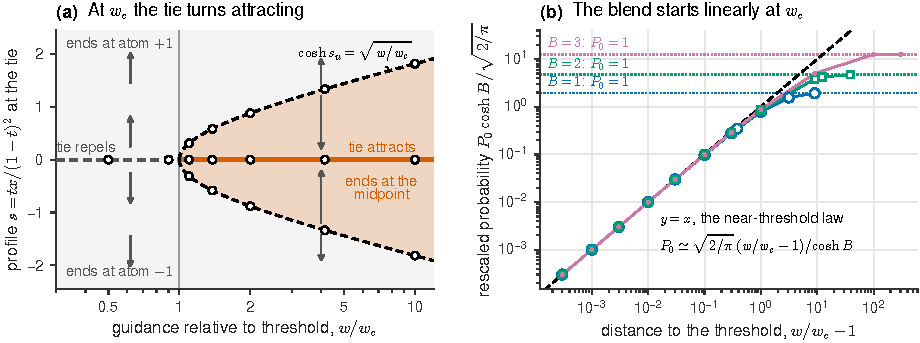
\includegraphics[width=\ificlr0.82\else0.98\fi\textwidth]{fig_composition.pdf}
\caption{Guided label averaging on two training points (Theorem~\ref{thm:composition}). (a) The
profiles, zeros of $F_w$ in \eqref{eq:composition-mean}, against $w/w_c$, $w_c=1/\sinh^2B$. The tie
$s=0$ repels below $w_c$ and attracts above it, as $F_w'(0)=\operatorname{sech}^2B\,(1-w/w_c)$; above
$w_c$ the repelling profiles $\pm s_u$, $\cosh s_u=\sqrt{w/w_c}$ (dashed), bound the profiles that end
at the midpoint (shaded). Arrows give the direction of the profile flow. In the coordinate $s$ the
profiles depend on $B$ only through $w/w_c$; circles are the zeros computed numerically for
$B=1,2,3$. (b) Probability $P_0$ under $\pi_0$ that the trajectory ends at the midpoint, divided by
the prefactor of the near-threshold law of Appendix~\ref{apx:threshold-scaling}, against $w/w_c-1$,
for $B=1$ (circles), $2$ (squares) and $3$ (dots): exact-flow computations with stopping criteria
justified by the proof, and bisection (Table~\ref{tab:composition} and
Appendix~\ref{apx:threshold-scaling}). Near the threshold the three curves collapse on the law
$P_0\simeq\sqrt{2/\pi}\,(w/w_c-1)/\cosh B$ (dashed); far from it each saturates at $P_0=1$ (dotted).
Below the threshold only the source $x_0=0$ reaches the midpoint.}
\label{fig:composition}
\end{figure}
}%

\subsection{A spectral criterion in any dimension}
\label{sec:spectral}

\moveblock{spectraldefs}{%
The trace $\Theta$ decides Step~2 only through its sign; in more than one dimension the relevant
object is the matrix whose trace it is. Fix a non-atom candidate $z\in\mathcal C'$ with tied
nearest atoms $S=\nn(z)$, so $|S|\ge2$ and $z\in\operatorname{aff}S$, and let
$L=\operatorname{span}\{a-z:a\in S\}$. Consider a field $\sum_kc_kv_{p_k}$ with finitely many
$p_k\in\Ppos$ and constant coefficients summing to one; this covers guidance, label averaging
over finitely many labels, and guided label averaging. For $\xi\in L$ let $\pi_k(\xi)$ be the
prior $p_k$ restricted to $S$ and tilted by $e^{\langle\xi,a\rangle}$, and put
\[
M(\xi)=\sum_kc_k\,\E_{\pi_k(\xi)}[a],\qquad
\Gamma(\xi)=D_LM(\xi)=\sum_kc_k\Cov_{\pi_k(\xi)}(P_La).
\]
The rescaled position $\xi=\beta P_L(x-tz)$ generalises $s$ of Section~\ref{sec:composition}; a
\emph{profile} is a root of $M(\xi)=z$, \emph{hyperbolic} if $\Gamma$ is invertible there.
}%
\ificlr Beyond two atoms the same question is decided by a matrix. At a non-atom candidate $z$ with
tied nearest atoms $S$, the rescaled position $\beta P_L(x_t-tz)$ of a trajectory converging to $z$
tends to a \emph{profile}, a root of the restricted posterior mean of the field, and the signed
posterior covariance $\Gamma$ at the profile plays the role of $F_w'(0)$.
Theorem~\ref{thm:spectral} in Appendix~\ref{apx:pf-spectral} shows that $\Gamma\prec0$ gives an
open basin, so the endpoint law has an atom at $z$, that a positive eigenvalue gives a null basin,
and that these cases are exhaustive under a face condition; Corollary~\ref{cor:spectral-threshold}
gives the matrix threshold, $1/\sinh^2B$ for two atoms. In $d\in\{2,8\}$, sources and saddles,
including those the trace test misses, put no source at $z$; sinks keep a positive fraction,
except for the simplex in $d=8$ at $w\le2w_c$, where it falls below the resolution $1/2048$
(Table~\ref{tab:spectral}).
\fi
\moveblock{spectralthm}{%
\begin{restatable}[Spectral classification of off-support endpoints]{theorem}{thmspectral}
\label{thm:spectral}
Let $\xi_\star$ be a hyperbolic profile, and call its basin the set of initial points with
$x_t\to z$ and $\beta P_L(x_t-tz)\to\xi_\star$.
\begin{enumerate}[label=(\alph*),leftmargin=2em]
\item If $\Gamma(\xi_\star)\prec0$ on $L$, the basin contains a nonempty open set, so the endpoint
  law from $\pi_0$ has an atom at the non-training point $z$.
\item If $\Gamma(\xi_\star)$ has a positive eigenvalue, the basin is Lebesgue-null.
\item If every profile is hyperbolic and $P_Lz\notin\operatorname{aff}F$ for every proper face $F$
  of $\operatorname{conv}P_LS$, every trajectory converging to $z$ has a profile converging to one
  of finitely many profiles. Then $\Pr(X_1=z)>0$ exactly when some profile has
  $\Gamma(\xi_\star)\prec0$ on $L$.
\end{enumerate}
\proofin{apx:pf-spectral}
\end{restatable}
}%

\moveblock{sketchspectral}{%
\begin{proofsketch}
In the time $\sigma$ with $d\sigma=\beta\,d\tau$ the profile obeys
$d\xi/d\sigma=M(\xi)-z+o(1)$, while the normal part $P_{L^\perp}(x-z)$ decays at the slow rate
$e^{-\tau}$. A Lyapunov--Perron argument for this fast--slow system shows that the trajectories
converging to a hyperbolic profile form a Lipschitz graph of codimension equal to the number of
positive eigenvalues of $\Gamma$, which gives (a) and (b). For (c), $M-z$ is the gradient of a
potential that grows linearly away from the profiles, whereas convergence to $z$ forces
$\xi=o(\sigma)$; so profiles cannot escape to infinity.
\end{proofsketch}
}%


\moveblock{spectralafter}{%
Lemma~\ref{lem:volume} uses only $\Theta=\tr\Gamma$: a profile with $\tr\Gamma>0$ already has a
null basin. Theorem~\ref{thm:spectral}(b) also covers saddles with $\tr\Gamma\le0$, and (a) gives
the positive-measure counterpart in any dimension. In one dimension trace and eigenvalue
coincide, and the roots $0$ and $\pm s_u$ of $F_w$ recover Theorem~\ref{thm:composition}, except
at the nonhyperbolic threshold $w=w_c$, which its proof treats separately.
}%
\moveblock{corspectral}{%
\begin{restatable}[Matrix threshold for guided label averaging]{corollary}{corspectral}
\label{cor:spectral-threshold}
Let $M_{\mathrm{av}}$ average the restricted means of finitely many conditional priors in $\Ppos$
and $M_{\mathrm u}$ be that of the unconditional prior, and suppose $M_{\mathrm{av}}(\xi_\star)=
M_{\mathrm u}(\xi_\star)=z$ for some $\xi_\star\in L$. Let $C_{\mathrm{av}}$, $C_{\mathrm u}$ be their
derivatives on $L$ at $\xi_\star$, and assume $D=C_{\mathrm u}-C_{\mathrm{av}}\succ0$ on $L$. For
\[
w>w_c^{\mathrm{spec}}=\lambda_{\max}\big(D^{-1/2}C_{\mathrm{av}}D^{-1/2}\big),
\]
the guided label average puts positive probability on $z$. For the two atoms of
Theorem~\ref{thm:composition}, $w_c^{\mathrm{spec}}=1/\sinh^2B$. \proofin{apx:pf-spectral}
\end{restatable}
The common equilibrium holds in symmetric configurations, such as a regular simplex with one
conditional prior favouring each vertex, where $w_c^{\mathrm{spec}}=(1-m^2)/m^2$ with
$m=(e^B-1)/(e^B+N-1)$; Section~\ref{sec:intervention-tests} checks the classification
numerically. Nonhyperbolic profiles and faces whose affine hull contains $P_Lz$ are not covered;
Remark~\ref{rem:generic} shows that both are exceptional.
}%

\begin{remark}[How restrictive the hypotheses of Theorem~\ref{thm:spectral}(c) are]
\label{rem:generic}
The face condition involves only the atoms. Since $a-z\in L$ for $a\in S$, the set
$P_LS=P_Lz+(S-z)$ is a translate of $S$, and the condition says that $z$ lies in the affine hull
of no proper face of $\operatorname{conv}S$. It holds when $|S|=2$, and whenever $z$ lies in the
relative interior of $\operatorname{conv}S$, because the affine hull of a proper face lies in a
supporting hyperplane of $\operatorname{conv}S$ within $\operatorname{aff}S$; this covers every
configuration of Section~\ref{sec:intervention-tests}. Hyperbolicity is generic in the priors.
Fix $a_0\in S$ and put $\eta_{k,a}=\log\bigl(p_k(a)/p_k(a_0)\bigr)$ for $a\in S\setminus\{a_0\}$;
the map $G(\xi;\eta)=M(\xi)-z$ from $L\times\R^{K(|S|-1)}$ to $L$ depends on the priors only
through $\eta$, and $\partial G/\partial\eta_{k,a}=c_k\,\pi_k(\xi)(a)\,\bigl(a-\E_{\pi_k(\xi)}[a]\bigr)$.
For any $k$ with $c_k\neq0$ these vectors span $L$: together with the vector for $a_0$ they sum to
zero, and their span contains every difference of two points of $S$, and these differences span
$L$ because $z\in\operatorname{aff}S$. So $G$ is a submersion, and the parametric transversality
theorem \citep[Ch.~2, \S3]{guillemin1974differential} shows that for almost every $\eta$ zero is a
regular value of $G(\cdot;\eta)$: every profile is hyperbolic. The log-ratio map from $\Ppos$ to
$\eta$ is a submersion, so the same holds for almost every choice of the priors
$(p_1,\dots,p_K)\in(\Ppos)^K$. Nonhyperbolic profiles, such as the threshold $w=w_c$ of
Theorem~\ref{thm:composition}, are therefore exceptional, although what happens at them, and at
faces through $z$, remains open.
\end{remark}


\subsection{Composing conditions}
\label{sec:conjunction}

Compositional generation combines several conditions $c_1,\dots,c_K$ by adding their guidance
terms: the conjunction of \citet{liu2022composable} integrates
$v_{\mathrm{unc}}+\sum_kw_k(v_{c_k}-v_{\mathrm{unc}})$, written here for velocities, which enter
linearly. With equal weights $w_k=(1+w)/K$ this is
\[
(1+w)\,\frac1K\sum_{k=1}^Kv_{c_k}-w\,v_{\mathrm{unc}},
\]
guidance with strength $w$ applied to the average of the $K$ conditional fields. For exact fields
with strictly positive priors this is the composite of Theorem~\ref{thm:composition} and
Corollary~\ref{cor:spectral-threshold}, with the average over nearby labels replaced by the average
over the conditions being combined. A single condition with a fixed $w\ge0$ or a bounded schedule
ends on a training example almost surely (Proposition~\ref{prop:cfgatom},
Theorem~\ref{thm:schedule}); the conjunction of two conditions whose priors favour different
training examples puts positive probability on their circumcentre once $w>w_c^{\mathrm{spec}}$.
In the two-atom case with log-odds $\pm2B$, $w_c=1/\sinh^2B\approx4e^{-2B}$: the more confidently
each condition identifies its own example, the smaller the guidance at which their conjunction
blends them. The regular simplex after Corollary~\ref{cor:spectral-threshold} is the conjunction of
$K=N$ conditions. Section~\ref{sec:regular-learned} asks what a learned field needs to reach these
blends, and Section~\ref{sec:intervention-tests} answers it numerically for networks trained by
flow matching.

\paragraph{Which combinations blend two examples.} The conjunction is one signed combination of
three fields, and Corollary~\ref{cor:twofields} rules out every combination of two. Which
combinations of three or more exact fields put mass on a blend? At a tie of two atoms the answer
is short. Let $z$ be the midpoint of atoms $a,b$ with $\nn(z)=\{a,b\}$, in any dimension, and for
$p\in\Ppos$ write $B(p)=\tfrac12\log\bigl(p(a)/p(b)\bigr)$ for its log-odds restricted to the tie.
Only these restrictions enter $M$ and $\Gamma$ of Section~\ref{sec:spectral}, so priors with equal
$B$ act identically at this tie, and we add their coefficients. In the coordinate
$\zeta=\langle\xi,(a-b)/2\rangle$ the profile equation reads
\[
F(\zeta)=\sum_kc_k\tanh\bigl(\zeta+B(p_k)\bigr)=0,
\]
and $\Gamma$ has the sign of $F'(\zeta)$.

\begin{restatable}[Blending two examples needs a subtracted, less decided field]{proposition}{proptwoatom}
\label{prop:twoatom}
Consider $\sum_kc_kv_{p_k}$ with finitely many $p_k\in\Ppos$ and constant coefficients summing to
one, at the midpoint $z$ of a tie of two atoms, with priors of equal $B(p_k)$ grouped.
\begin{enumerate}[label=(\alph*),leftmargin=2em]
\item At a profile $\zeta_\star$, $F'(\zeta_\star)=1-\sum_kc_k\tanh^2\bigl(\zeta_\star+B(p_k)\bigr)$.
  If every prior whose $B(p_k)$ lies strictly between $\min_kB(p_k)$ and $\max_kB(p_k)$ has a
  nonnegative coefficient, then $F'>0$ at every profile, and $\Pr(X_1=z)=0$.
\item With three distinct values $B(p_1)>B(p_2)>B(p_3)$, if $c_2\ge0$, $c_1\le0$ or $c_3\le0$,
  then $F'>0$ at every profile, and $\Pr(X_1=z)=0$.
\item The conjunction, $c_1=c_3=\tfrac{1+w}2$, $c_2=-w$, $B(p_1)=-B(p_3)=B>0$, $B(p_2)=0$, has a
  profile with $F'<0$ exactly when $w>1/\sinh^2B$.
\end{enumerate}
\proofin{apx:pf-twoatom}
\end{restatable}

A blend of two examples thus needs a subtracted field that is less decided between them than the
fields it is subtracted from. In the conjunction the unconditional field, $B=0$, lies between two
conditions favouring $a$ and $b$, and it is subtracted. Negative prompting with an unconditional
base integrates
$v_{\mathrm{unc}}+s\,(v_{\mathrm{pos}}-v_{\mathrm{unc}})-s_{\mathrm{neg}}(v_{\mathrm{neg}}-v_{\mathrm{unc}})$
and subtracts the negative-prompt field. If the positive prompt favours $a$ and the negative
prompt favours $b$, the subtracted field is the extreme one, and by~(b) a blend of $a$ and $b$ has
probability zero. If the negative prompt favours $a$ less than the positive prompt does,
$0<B(p_{\mathrm{neg}})<B(p_{\mathrm{pos}})$, the subtracted field is the middle one, and blends can
occur (Section~\ref{sec:intervention-tests}). A negative prompt that does not distinguish $a$ from
$b$, $B(p_{\mathrm{neg}})=0$, is grouped with the unconditional field and changes nothing at this
tie: a condition unrelated to the tied examples acts there as the unconditional field does,
whatever the sign of its coefficient. Conditions (a) and (b) are necessary, not sufficient;
Figure~\ref{fig:signed} shows how much of the allowed region actually blends. The conjunction on the
regular simplex after Corollary~\ref{cor:spectral-threshold} therefore also blends pairs of
vertices: at the midpoint of an edge the other $N-2$ conditions have $B(p)=0$ and are grouped with
the unconditional field, so~(c) applies with $B/2$ in place of $B$ and $2(1+w)/N-1$ in place of
$w$. Theorem~\ref{thm:spectral} then gives the edge midpoints positive probability for
$w>N/(2\tanh^2(B/2))-1$ and probability $0$ for smaller $w$; for the triangle at $B=2$ this
threshold is $1.368\,w_c$ (\ificlr Appendix~\ref{app:intervention-protocol}\else
Section~\ref{sec:intervention-tests}\fi).

\begin{figure}[t]
\centering
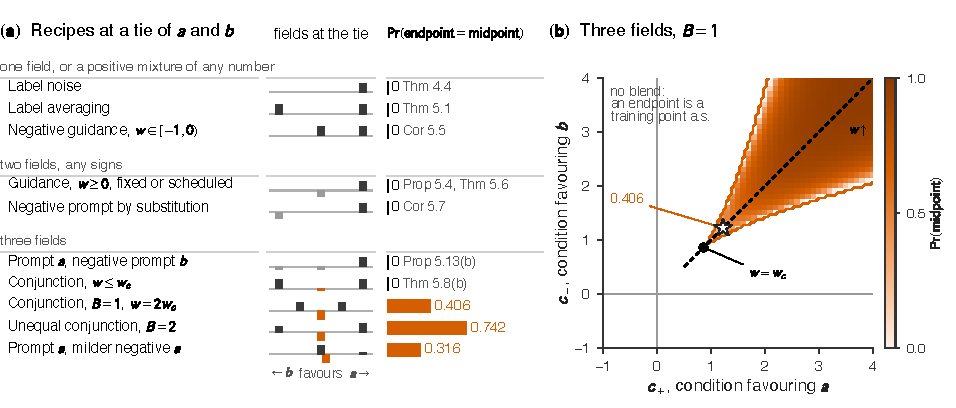
\includegraphics[width=0.98\textwidth]{fig_signed_combinations.pdf}
\caption{Which recipes can blend two training points $a,b$ at a tie. (a) Each row draws the fields of
a recipe as bars at their restricted log-odds $B(p)$, up when the field is added and down when it is
subtracted, with height proportional to the coefficient (per row); vermillion marks the sign
pattern Proposition~\ref{prop:twoatom} requires for a blend, a subtracted field less decided than
two added ones. Right: the probability under $\pi_0$ that the endpoint is the midpoint, $0$ where
the cited result proves it for every configuration (the bars then show one configuration, with
$B=2$, guidance $w=2$, negative guidance $w=-1/2$ and the conjunction at $w=w_c$), and otherwise
computed for the configuration drawn with the stiff
integrator and proof-based stopping rules of Section~\ref{sec:intervention-tests}. (b) The same
probability for three fields with restricted log-odds $B(p)=B,0,-B$ at $B=1$: coefficients
$c_+$, $c_-$ of the conditions favouring $a$ and $b$, and $1-c_+-c_-$ of the unconditional field,
on a grid of step $0.1$. Line: boundary of the region where the profile function $F$ has a zero
with negative slope (Theorem~\ref{thm:spectral}); outside it the probability is $0$, and inside it
$18$ cells next to the boundary are left white, their probability being below $0.01$. No point of
the region has $c_+\le0$ or $c_-\le0$, as Proposition~\ref{prop:twoatom}(b) requires. Dashed: the
equal conjunction $c_+=c_-=(1+w)/2$, $w\ge0$, which enters the region at $w=w_c=1/\sinh^2B$ (dot);
star: $w=2w_c$, the row of (a) with probability $0.406$.}
\label{fig:signed}
\end{figure}

\moveblock{whatleaves}{%
\subsection{What leaves the support}
\label{sec:interventions}

Table~\ref{tab:interventions} summarises what each intervention does to the support of the exact
endpoint law. Endpoint noise, $X_1=x^I+\rho\xi$, is the only one among them that leaves the
atoms in every configuration: its endpoint law has a density (Proposition~\ref{prop:tgtnoise}).
Averaging hard-label fields can also move every endpoint, but only in configurations such as the
symmetric tie of Section~\ref{sec:posmix}.
}%


% ==========================================================================
\section{What a learned field needs to reach a blend}
\label{sec:regular-learned}

A trained network differs from the exact field, and small regression loss does not control where
that difference sends the endpoint \citep[Theorem~1]{benton2024error}. The following statement
says what regularity a learned field may keep near $t=1$ and still end on an atom, whether a
training example or the circumcentre of Theorem~\ref{thm:composition}.

\moveblock{regular}{%
\begin{restatable}[Regular learned fields]{proposition}{propregular}
\label{prop:regular}
Let $v_\theta$ be continuous and locally Lipschitz in $x$ on $\R^d\times[0,1)$.
\begin{enumerate}[label=(\alph*),leftmargin=2em]
\item If its spatial Lipschitz constant $L(t)$ and $|v_\theta(0,t)|$ are integrable on $[0,1)$,
  the endpoint map $x_0\mapsto X_1$ is a bi-Lipschitz homeomorphism of $\R^d$; under every
  absolutely continuous source the endpoint law is absolutely continuous and has no atom.
\item Let $d=1$ and $v_\theta=(\hat x_1-x)/(1-t)$ on $[t_0,1)$, where $\hat x_1$ is bounded and
  continuous and $\partial_x\hat x_1$ is continuous on $\R\times[t_0,1]$, and let
  $g=\hat x_1(\cdot,1)$ have finitely many fixed points. Every trajectory converges to a fixed
  point of $g$; a fixed point $z$ with $g'(z)>1$ is the limit of at most one initial point, and
  one with $g'(z)<1$ is the limit of a nonempty open interval of initial points.
\end{enumerate}
\proofin{apx:pf-regular}
\end{restatable}

An MLP with Lipschitz activations that outputs a velocity from a smooth embedding of
$t\in[0,1]$, such as the standard conditional flow matching (CFM) network of Section~\ref{sec:intervention-tests}, satisfies
(a): its endpoint law has no atom anywhere, so any collapse it shows at a finite cutoff is an approach to an atom, not an atom. The same MLP predicting data satisfies (b) once its output is clipped to a bounded range,
and so does its guided label average, with
$g_w=(1+w)\bar g_\varphi-w\,g_{\mathrm{unc}}$ formed from the networks' predictions at $t=1$. The
exact composite carries no threshold there: every exact mean tends to the nearest atom off the
tie, for every label and every $w$, and $w_c=1/\sinh^2B$ is set at the scale $|x|\sim(1-t)^2$
around the tie. Under (b) the off-atom basin is therefore decided by the slope
$g_w'(0)=(1+w)\bar g_\varphi'(0)-w\,g_{\mathrm{unc}}'(0)$ of the networks' limits, which the exact
field does not constrain. Reproducing the exact threshold requires a prediction whose spatial
derivative is unbounded near the tie as $t\uparrow1$, as for an input $\operatorname{asinh}(tx/(1-t)^2)$.
}%

% ==========================================================================
\section{Numerical evidence}
\label{sec:intervention-tests}
\label{sec:experiments}

This section checks the theorems numerically and asks how trained networks relate to them. The
exact-field computations are finite-time evaluations that should agree with the theorems; they do
not prove them. The learned runs ask what Proposition~\ref{prop:regular} leaves open: whether a
network trained by flow matching follows the label-noise reference of Theorem~\ref{thm:endpoint},
and whether it reproduces the blend basin of Theorem~\ref{thm:composition}. Protocols are in
Appendix~\ref{app:expdetails}.

\paragraph{The label-noise reference in trained networks.} Theorem~\ref{thm:endpoint} gives a
reference without free parameters for a network trained with label noise: the variance
$\tr\Covh(y)$ of the label-weighted training examples. We compare it with the variance of samples
from trained networks on two problems (Appendix~\ref{app:kernel-protocol}). On a linear-Gaussian
problem in $d=2$ with $N=200$ training pairs and five seeds, the ratio of the generated variance
to $\tr\Covh$ is $1.002\pm0.050$, $0.994\pm0.039$ and $1.011\pm0.022$ at $h=0.05$, $0.1$ and $0.5$
(Table~\ref{tab:p7kernel}). At $h=0.01$ the reference is nearly degenerate, with an effective
number of atoms $n_{\mathrm{eff}}=1/\sum_i(p_i^{(h)})^2\approx3.5$; the per-seed ratios range from
$0.92$ to $1.96$, and the comparison does not decide. These networks match a second moment of an
atomic law, which does not show that their samples lie on the atoms. On CIFAR-10 inpainting with a
$35.75$M-parameter U-Net and $N=2000$ training images, the exact field puts the across-condition
log--log slope of generated against reference variance at $1$. Networks retrained on three
independently drawn training sets give $0.34$, $0.32$ and $0.43$ at $h=4$ (mean $0.36$, $95\%$
$t$-interval $[0.22,0.51]$), so at image scale the generated variance does not follow the reference
across conditions (Table~\ref{tab:cifar-kernel}). At $h=6$ the reference spans less than two
decades, and the slope, between $0.08$ and $0.60$ across the training sets, is not determined. In a
further retraining with the same configuration, the networks leave $0.168$ of their samples at
$h=4$ and $0.276$ at $h=6$ off the training images at the cutoff $1-t=10^{-4}$, by a
nearest-neighbour criterion (sample standard deviations $0.012$ and $0.008$ over three seeds),
while the exact field at the same bandwidth leaves none. These samples come from the error of the
learned field and the finite cutoff: at the exact optimum, label noise keeps every endpoint on a
training image (Proposition~\ref{prop:atomicity}).

\paragraph{Exact fields.} Five geometry seeds, $d\in\{2,8\}$, $N=12$, random and near-duplicate
atoms, and $h\in\{0.3,1\}$ give 200 paired cells across single-field, guidance ($w=3,12$),
label-average and prior-average arms. With $128$ common sources and terminal gap $10^{-6}$, the
largest cellwise 95th percentile of the nearest-atom distance is $6.11937\times10^{-6}$
(Figure~\ref{fig:intervention-validation}, left, in Appendix~\ref{app:intervention-protocol}), and no sample exceeds the prespecified threshold of $1\%$ of the minimum atom separation. \moveblock{stressextra}{Doubling the
log-time RK4 resolution leaves every atom assignment unchanged. Field and prior averages differ
in paired assignments by up to $31.25\%$, so they are distinct interventions.}\ificlr\else{} These are
finite-time consistency checks, not a numerical proof. \fi\moveblock{neartie}{Near the symmetric tie of two atoms,
sources at small offsets stay close to the midpoint until very small gaps
(Figure~\ref{fig:intervention-validation}, middle), and four of six
adaptive near-tie integrations fail at small bandwidths; we report these failures
(Appendix~\ref{app:intervention-protocol}).}\ificlr Near-tie failures are in Appendix~\ref{app:intervention-protocol}.\fi

\paragraph{A positive control for the stress test.} None of the arms above has an attracting
non-atom candidate, so a scheme biased towards the atoms would pass the test as well. We therefore
gave the same fixed-step log-time RK4, with the same $256$ and $512$ steps per segment and the
same terminal gaps, the guided average of two conditional fields on the atoms $(\pm1,0)$ in $d=2$,
with $B=1$, $w/w_c\in\{0.9,1.1,2,10\}$ and $4096$ Gaussian sources. At every gap and both step
sizes it sends to the midpoint exactly the sources that the stiff integrator below assigns to its
basin, with no disagreement among the $4096$: fractions $0$, $0.049$, $0.410$ and $0.988$, against
basin probabilities $0$, $0.050$, $0.406$ and $0.991$ under $\pi_0$, the differences being
sampling error. Along the line of the atoms the captured trajectories end within $3\times10^{-17}$
of the midpoint, while the orthogonal coordinate decays like $1-t$, and at the gaps $10^{-4}$ and
$10^{-6}$ the $1\%$ criterion flags exactly them. The stress test therefore sees an
attracting tie when there is one (Appendix~\ref{app:intervention-protocol}).

\paragraph{Guided label averaging.} For the configuration of Theorem~\ref{thm:composition} we
integrate the exact composite flow \ificlr with stopping rules taken from the proof, and locate
the basin of the midpoint, an interval, by bisection.\else with a stiff solver (Radau, relative tolerance $10^{-11}$)
and stop at the first time a sufficient condition from the proof fixes the limit: $s$ beyond the
outer roots of $F_w$, or $s$ inside the moving barrier around a root with $F_w'<0$. Flows on the
line preserve order, so the basin of the midpoint is an interval, located by bisection.\fi{}
\ificlr The horizontal coordinates in Figure~\ref{fig:learned-composition} give\else Figure~\ref{fig:composition}(b) gives\fi{} its $\pi_0$-probability, and Table~\ref{tab:composition}
in Appendix~\ref{app:intervention-protocol} lists the values. Below the threshold $w_c=1/\sinh^2B$
only the source $0$ reaches the midpoint (Theorem~\ref{thm:composition}(b); the stopping rule then
labels every other source an atom at its first check); just above it the computed basin probability grows
linearly\ificlr{}, as a formal law predicts (Appendix~\ref{apx:threshold-scaling}).\else, as $\sqrt{2/\pi}\,(w/w_c-1)/\cosh B$ to within $0.01\%$ at $w=1.0003w_c$, a formal
law derived in Appendix~\ref{apx:threshold-scaling}.\fi{} \moveblock{compperturb}{The numerical unstable roots agree with the closed form $\cosh s_u=\sqrt w\sinh B$.
With $w=1$ and $B\approx2$, unequal mixture weights $(0.6,0.4)$, unequal $(B_1,B_2)=(2,-1.5)$, an
unconditional log-odds $2B_u=0.6$, or a combination of all three keep basin probabilities between
$0.71$ and $0.86$, as Proposition~\ref{prop:composition-open} predicts.}\ificlr Perturbed
configurations keep basin probabilities between $0.71$ and $0.86$
(Appendix~\ref{app:intervention-protocol}).\fi{} \ificlr On eight selected and twelve random CIFAR-10 pairs, a consistency check whose
classifier admits the midpoint only above the threshold of Theorem~\ref{thm:spectral}(c), the exact
composite ends a positive fraction of the sources there in every pair at $2w_c$ (Appendix~\ref{app:cifar-composition}).\else On eight selected
and twelve random CIFAR-10 pairs, with all $2000$
training images in the field, Theorem~\ref{thm:spectral}(c) predicts the same threshold; in this
consistency check, whose classifier admits the midpoint only above the threshold, the exact composite ends
a positive fraction of the sources there in every pair at $2w_c$, up to $0.29$
(Appendix~\ref{app:cifar-composition}).\fi

\paragraph{Learned guided label averaging.} We train networks by flow matching on the two atoms
of Theorem~\ref{thm:composition} ($\ell=h=1$) and on an equilateral triangle with one
conditional prior favouring each vertex ($B=2$), five seeds each, and integrate the learned
composite with an adaptive stiff solver (Appendix~\ref{app:learned-composition}). A standard \ificlr conditional flow matching (CFM)\else CFM\fi{} network, with velocity output and
condition dropout, places at most $0.001$ of the sources at the midpoint at $B\in\{1,2\}$ and none
at the centre of the triangle, at every guidance strength (Figure~\ref{fig:learned-composition})\ificlr.\else; at $B=1$,
neither log-uniform sampling of $1-t$ nor a separate unconditional network changes this.\fi{} A
network that predicts the data with the loss $|\hat m-X_1|^2$, which has the same minimiser, and
receives the blow-up coordinate $\operatorname{asinh}(tx/(1-t)^2)$, centred at the known tie
$z=0$ (centred elsewhere it leaves the midpoint empty, Appendix~\ref{apx:bottleneck-runs}), as an extra input follows the exact probabilities: $0.401\pm0.006$ against $0.406$ at $B=1$ and $w=2w_c$, and $0.143\pm0.004$
against $0.133$ at the centre of the triangle at $2w_c$. It follows the exact flow only at the tie
its input is centred on: the exact composite ends a further $0.426$ of the first $4096$ shared
sources at the edge midpoints of the triangle at $2w_c$ and $0.306$ at $5w_c$, whereas the standard
network, this network and the distillation control of Appendix~\ref{app:learned-composition} place
at most $3$ of their $2048$ sources within $0.05$ of an edge midpoint at $1-t=10^{-5}$, in any seed
and at any guidance strength. Nor do their other endpoints all lie at training points: at
$1-t=10^{-5}$ the standard network leaves $0.16$, $0.70$ and $0.79$ of its sources at $2$, $5$ and
$10\,w_c$ farther than $0.1$ from every atom and from the centre, and the data-predicting network
$0.16\pm0.16$ at $2w_c$. \moveblock{lossrisk}{The velocity
network has the smaller held-out excess risk for $t\ge0.999$ ($1.4\times10^{-7}$ against
$9.4\times10^{-7}$), yet its posterior mean misses the boundary layer at the tie: at
$1-t=10^{-5}$ its mean squared error over $|s|\le3$ is $0.67$, against $0.0024$. Small loss does not
decide the endpoint \citep[Theorem~1]{benton2024error}.} Of the changes the successful network
makes, the input matters most in these runs: a velocity network with it matches the exact probabilities in most seeds
($0.881\pm0.003$ against $0.878$ at $B=1$, $w=5w_c$), while a data-predicting network without it
leaves the midpoint empty at $w\ge5w_c$, consistent with Proposition~\ref{prop:regular}(b)
(Appendix~\ref{app:learned-composition}).

\begin{figure}[t]
\centering
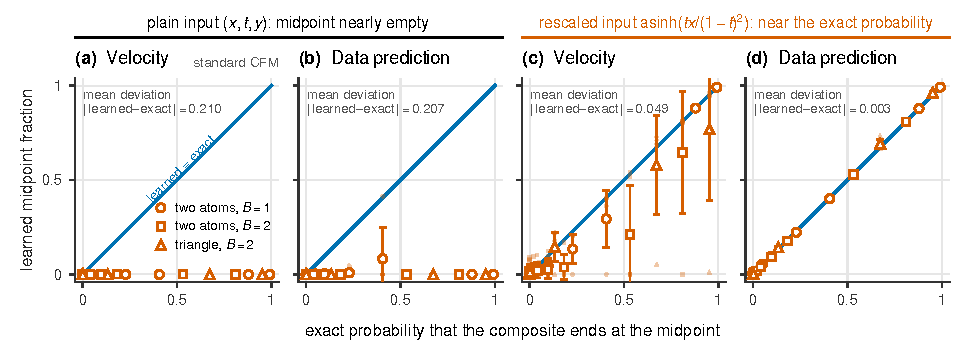
\includegraphics[width=\ificlr0.72\else0.98\fi\textwidth]{fig_learned_composition.pdf}
\caption{Learned against exact guided label averaging for four networks: velocity or data output,
without (a, b) or with (c, d) the rescaled input $\operatorname{asinh}(tx/(1-t)^2)$; (a) is
standard CFM. Each marker is one configuration (the two atoms of Theorem~\ref{thm:composition} with
$B=1$ or $2$, or the triangle with $B=2$) at one guidance strength $0\le w/w_c\le10$: horizontally
the exact probability that the composite ends at the midpoint (for the triangle, its centre; the
exact composite also ends mass at the edge midpoints, which the networks of (a) and (d), whose
endpoints were stored, leave empty, Section~\ref{sec:intervention-tests}),
vertically the learned \ificlr fraction, mean and standard deviation over five seeds, dots for
single seeds (six of the strengths are in Table~\ref{tab:learned-composition}).\else fraction of
$2048$ shared sources within $0.05$ of the midpoint at $1-t=10^{-5}$, mean and standard deviation
over five seeds, dots for single seeds (six of the strengths are in
Table~\ref{tab:learned-composition}).\fi{} On the diagonal a network has the
exact probability; grey: the mean absolute deviation from it. Without the rescaled input the
midpoint stays nearly empty (one seed in (b) places $0.415$ at $B=1$, $w=2w_c$); with it the
velocity network follows the diagonal in most seeds, and the data-predicting network in all seeds
shown; at $B=3$, not drawn, one of its five seeds places no source at the midpoint at $2$ and
$5\,w_c$ (Table~\ref{tab:learned-composition}).}
\label{fig:learned-composition}
\end{figure}

\moveblock{spectralexp}{%
\paragraph{The spectral criterion beyond the line.} We integrate the exact flow of
Theorem~\ref{thm:spectral} in four configurations whose atoms all lie on the unit sphere around
$z=0$, so that every atom is tied and the blown-up equation has no off-tie term. Two are a
triangle in $d=2$ and a regular nine-vertex simplex in $d=8$, each with one conditional prior
favouring each vertex ($B=2$). The other two are a rectangle in $d=2$ and a $256$-vertex box in
$d=8$ with product priors; at $w=1$ the profile $\xi=0$ is a saddle with negative $\tr\Gamma$,
where the trace test of Lemma~\ref{lem:volume} is silent. Every source or saddle profile ends
with no source at $z$. Every sink profile in $d=2$ keeps a stable positive fraction of the sources
($0.001$, $0.140$, $0.687$ for the triangle at $1.1,2,5\,w_c$). In $d=8$ the basins of $z$ are
smaller: $0.019$ for the simplex at $5\,w_c$ and $0.002$ (one of $512$ sources) for the box at
$w=5$, and below the sampling resolution of $1/2048$ for the simplex at $1.1$ and $2\,w_c$
(Table~\ref{tab:spectral}). These fractions count the
centre only, and on the triangle the centre is not the only blend: the edge midpoints are ties of
two atoms that attract for $w>1.368\,w_c$ and have probability $0$ below this value
(Section~\ref{sec:conjunction}). With $32768$ sources, each classified by the candidate it
converges to (Appendix~\ref{app:intervention-protocol}), the exact flow ends $0.131$, $0.409$ and
$0.460$ of the mass at the centre, the edge midpoints and the training points at $2w_c$
(Figure~\ref{fig:unrolled}c), $0.681$, $0.294$ and $0.025$ at $5w_c$, and $0.950$, $0.050$ and
$0.0001$ at $10w_c$, with standard errors at most $0.003$; at $1.1\,w_c$ no source ends at an edge
midpoint. The other configurations have further blends. On the simplex the centroid of a face with
$k$ vertices is a tie of $k$ atoms at which the other $9-k$ conditions act as the unconditional
field, and its profile $\xi=0$ attracts for $w>9/(k\,m_k^2)-1$, $m_k=(e^B-1)/(e^B+k-1)$: for
$w>1.407\,w_c$ at an edge and for $w$ above $0.97$ to $1.14\,w_c$ when $3\le k\le8$. With product
priors the flows of the rectangle and the box separate by axis into one-dimensional composites as
in Theorem~\ref{thm:composition}, with $B(p)=\pm2$ on the long axes and $\pm1/2$ on the short ones,
so a long axis ends at $0$ with positive probability for $w>1/\sinh^22=0.076$, also at $w=1$, where
$\xi=0$ is a saddle, and a short one for $w>1/\sinh^2(1/2)=3.68$; the centroids of the faces
spanned by such axes are blends. When every endpoint is classified by the face whose centroid it
reaches, with the integration and the numbers of sources of Table~\ref{tab:spectral}
(Appendix~\ref{app:intervention-protocol}), these other blends take $0.953$ of the mass of the
simplex at $2\,w_c$ and $0.981$ at $5\,w_c$ (and $0.001$ at $1.1\,w_c$), $0.895$ and $0.754$ of
the rectangle at $w=1$ and $5$, all at the midpoints of its long edges, and all $512$ sources of
the box at $w=1$ and $511$ of them at $w=5$. These are finite-time computations that agree with
the theorem; they do not prove it.
}%

\paragraph{Signed combinations at a two-atom tie.} Proposition~\ref{prop:twoatom} gives
necessary conditions, and we checked how far they are from sufficient. Among $3841$ random
combinations of two to five priors with restricted log-odds in $[-4,4]$, $143$ have a profile
with $F'<0$; every one of them subtracts an inner prior, and every three-prior case has the sign
pattern of~(b). Figure~\ref{fig:signed} maps the three-prior family $B(p)\in\{B,0,-B\}$: a blend
needs both conditions added, as (b) requires, and adding them is not enough below a boundary that
meets the conjunction diagonal at $w=w_c$. With the stiff integrator and the proof-based stopping
rules of the previous paragraph, the midpoint has probability $0.406$ for the equal conjunction at
$B=1$, $w=2w_c$, and $0.742$ for the unequal conjunction $(c_+,c_-)=(1.2,0.8)$ at $B=2$. A positive
prompt for $a$ and a negative prompt for $b$ ($B=\pm2$) give probability $0$, both with an
unconditional base, coefficients $(3,-1,-1)$, and in the substituted form $3v_a-2v_b$. A positive
prompt for $a$ with a negative prompt that favours $a$ less ($B=2$ and $0.25$, coefficients $0.91$
and $-4$, unconditional coefficient $4.09$) gives $0.316$.

\moveblock{learnedpilot}{%
\paragraph{Learned label averages.} We reuse five $h=0.1$, 200k-step networks of the linear-Gaussian problem (Appendix~\ref{app:kernel-protocol}) and average
their predictions at $y-r,y,y+r$, with $r$ scaled by the training-label standard deviation, at
two training and two fresh queries per seed with 128 paired sources. Against the exact average of
the same three fields at $T=0.999$ (Table~\ref{tab:learned-averages}), wider averaging increases
the mean discrepancy, although not on every seed: exact atomicity does not transfer automatically
to a network. The biased energy statistic has no null subtraction or equivalence threshold.
}%


\moveblock{learnedtab}{%
\begin{table}[t]
\centering\small
\begin{tabular}{@{}rrrr@{}}
\toprule
$r/\operatorname{sd}(y)$ & Training energy & Fresh energy & Fresh seed range\\
\midrule
0 & 0.005627 & 0.007227 & 0.001876--0.009327\\
0.5 & 0.011200 & 0.011054 & 0.001887--0.018859\\
1.5 & 0.289771 & 0.143176 & 0.001758--0.544995\\
\bottomrule
\end{tabular}
\caption{Learned versus exact label averages across five problem seeds. Energy is normalised by
the square root of the analytic posterior trace; conditions and samples are nested within
seeds, so these are descriptive values, not hypothesis tests.}
\label{tab:learned-averages}
\end{table}
}%

% ==========================================================================
\section{Limitations}
\label{sec:limitations}

\emph{Exact fields, not trained networks.} The theorems concern exact fields of a fixed training
set and do not say that a trained network implements them. Learned label averages need not follow
the exact ones (Appendix~\ref{app:intervention-protocol}). Whether a network reproduces the blend
basin depends on its parametrisation, chiefly on an input centred at the tie, and not in every
seed; on the triangle the data-predicting network with this input leaves the blends at the other
ties, the edge midpoints, empty. \emph{Hypotheses.} The positive-bandwidth results need strictly
positive priors on a common support. Mixtures with different supports, schedules that are
unbounded or change sign, and, in the spectral classification, nonhyperbolic profiles and faces
whose affine hull contains the projected candidate are not covered. The latter are exceptional
(Remark~\ref{rem:generic}), but not shown to be harmless. The endpoint weights of averaged fields
are not identified. Proposition~\ref{prop:twoatom} concerns ties of two atoms and gives necessary
conditions only; for ties of three or more atoms, and for sufficiency, the spectral criterion has
to be evaluated case by case. \emph{Scope of the composition results.} The conjunction and the
negative prompts are analysed for exact conditional fields. Trained compositional samplers on
images, where the conditions are text prompts rather than labels, are not tested. \emph{Numerics.}
The exact-field computations are finite-time numerical evaluations, not interval arithmetic,
although a positive control shows that the fixed-step scheme of the stress test detects an
attracting tie. The learned composition experiments use three to five seeds and $d\le2$, and the
image-scale composition check uses the exact field on CIFAR-10 pairs, not a trained network. The
label-noise comparison uses one small synthetic problem and one image configuration with three
draws of the training set. At image scale the generated variance does not follow the reference,
and we do not identify why; the off-atom CIFAR-10 samples are measured at a finite cutoff and do
not identify a limiting support.

% ==========================================================================
\section{Conclusion}
\label{sec:conclusion}

Within the exact empirical field, the number of combined fields and their signs decide whether the
endpoints leave the training set. Label noise, label averaging, every fixed combination of two
exact fields with strictly positive priors, which includes negative prompting by substitution, and
guidance with a nonnegative bounded schedule of bounded variation reweight the training examples
and end on them almost surely, and every trajectory converges. Three fields can move the endpoints.
Guidance applied to an average of conditional fields, the conjunction of compositional generation,
reaches blends of training examples above an explicit threshold. A signed posterior covariance
decides when in any dimension, and at a tie of two examples a blend needs a subtracted field that
is less decided between them than the fields added.

For practice, none of these knobs guarantees at the exact optimum that training data are not
returned, and the composition of conditions is the operation an audit should examine. The blend
basin lives at the scale $(1-t)^2$ at the tie. Standard velocity networks did not resolve it in our
runs, while networks given a coordinate at that scale can do so at the tie where it is centred.
Whether trained compositional samplers produce such blends is therefore a question about their
inductive biases that the exact field does not settle.

\emph{Open questions.} Nonhyperbolic profiles and degenerate faces; sufficient conditions for a
blend beyond the conjunction, and necessary ones at ties of three or more atoms; how the endpoint
weights of averaged fields depend on the averaging scale; how basins scale with many atoms near a
candidate; why trained image networks with label noise depart from the label-noise reference; and
learned composition beyond $d\le2$, in particular for text-conditioned image samplers.

\subsection*{Broader impact statement}
This work studies when conditional flow-matching samplers return training examples. The
consequence for sensitive data is negative: at the exact optimum, label noise, label averaging,
negative guidance and bounded nonnegative guidance schedules of bounded variation give no guarantee
against replication, because
they only reweight the training examples, and the blends reached by composing conditions are
combinations of training records. Under label noise the returned record is predictable from the
query and the training labels, which helps auditors and, equally, an adversary who knows the
labels. Moving the support requires a change such as endpoint noise, which does not by itself hide
the source record, and a formal guarantee requires randomisation calibrated in the sense of
differential privacy, which we do not analyse. All experiments use synthetic data and the public
CIFAR-10 dataset; no personal or human-subject data are involved.

\subsection*{Use of large language models}
% DECISION: (contract 7.5) the wording of the LLM statement is a group decision; unchanged here.
% DECISION: (contract 7.6) the group must check the proofs of cor:twofields, prop:twoatom and
% rem:generic itself before submission.
We used large language models as assistants for writing and running experiment and analysis code,
for editing the manuscript, and as additional checkers of the written proofs. The statements and
proofs of Corollary~\ref{cor:twofields}, Proposition~\ref{prop:twoatom} and
Remark~\ref{rem:generic} were first drafted with a large language model. The authors take full
responsibility for the content of the paper.

\subsection*{Reproducibility statement}
\begingroup\raggedright
All numbers are produced by code in the supplementary material (anonymised for review):
Figure~\ref{fig:unrolled}, the endpoint laws on the triangle, the blend masses of the spectral
configurations and the learned edge counts (\texttt{theory\_basin\_map.py},
\texttt{make\_theory\_hero\_figure.py}), the composition computations and
Figure~\ref{fig:composition} (\texttt{composition\_counterexample.py},
\texttt{composition\_threshold\_scaling.py}, \texttt{make\_composition\_figure.py}), the spectral
checks (\texttt{spectral\_criterion\_check.py}),
the intervention stress tests and Figure~\ref{fig:intervention-validation}
(\texttt{novelty\_interventions.py}, \texttt{novelty\_ties\_refined.py},
\texttt{summarize\_novelty\_interventions.py}, \texttt{make\_intervention\_validation\_figure.py},
and the positive control \texttt{stress\_positive\_control.py}), the signed combinations and
Figure~\ref{fig:signed} (\texttt{signed\_combinations\_check.py},
\texttt{signed\_combinations\_probability.py}, \texttt{make\_signed\_combinations\_figure.py}), the
learned composition and Figure~\ref{fig:learned-composition} (\texttt{learned\_composition.py},
\texttt{learned\_composition\_2d.py}, \texttt{learned\_composition\_exact.py},
\texttt{summarize\_learned\_composition.py}, \texttt{make\_learned\_composition\_figure.py}), the
CIFAR-10 pairs and
Figure~\ref{fig:cifar-composition} (\texttt{cifar\_composition\_exact.py},
\texttt{make\_theory\_cifar\_composition\_figure.py}), the label-noise comparisons of
Tables~\ref{tab:p7kernel} and~\ref{tab:cifar-kernel} (\texttt{analyze\_p7\_kernel.py},
\texttt{reeval\_exp3\_cifar\_ddpm.py}, \texttt{paperB\_uncertainty.py},
\texttt{summarize\_s10\_cifar.py}) and the kernel and endpoint-noise checks
(\texttt{test\_kernel\_theory.py}, \texttt{verify\_kernel\_theory.py},
\texttt{verify\_target\_noise.py}). Every assumption is stated where it is used, and all results are
proved in the appendices.\par\endgroup

\bibliographystyle{tmlr}
\bibliography{refs}

% ==========================================================================
\appendix
\proofpointerfalse

\section*{Organization of the appendix}
\addcontentsline{toc}{section}{Organization of the appendix}

Appendix~\ref{app:proofs} proves the statements of Section~\ref{sec:theory} on the exact
reference. Appendix~\ref{app:intervention-proofs} proves the intervention results of
Section~\ref{sec:intervention-atomicity}: it first isolates two general lemmas that every
intervention proof uses, then treats positive mixtures, guidance and their composition, and ends
with the spectral classification. Appendix~\ref{app:regular} proves
Proposition~\ref{prop:regular}, Appendix~\ref{app:noise} treats endpoint noise, and
Appendix~\ref{app:expdetails} gives the numerical protocols, including the label-noise
comparison with trained networks (Appendix~\ref{app:kernel-protocol}). Each main-text result is restated,
with its original number, immediately before its proof. Table~\ref{tab:notation} collects the
notation and Table~\ref{tab:roadmap} shows where each result is proved and what it uses.

\begin{table}[h]
\centering\small
\begin{tabular}{@{}p{0.29\textwidth}p{0.64\textwidth}@{}}
\toprule
Symbol & Meaning\\
\midrule
$\D=\{(x^i,y^i)\}_{i=1}^N$, $d$, $k$ & training set, data dimension, label dimension\\
$\rhohat_X=N^{-1}\sum_i\delta_{x^i}$ & empirical law of the training inputs (the atoms)\\
$\pi_0=\N(0,I_d)$ & source law\\
$X_t=(1-t)X_0+tX_1$, $U=X_1-X_0$ & linear interpolant and regression target\\
$h$, $K_h$, $\widetilde Y=Y+h\omega$ & label bandwidth, Gaussian label kernel, noised label\\
$\vstar$, $v_{\mathrm{unc}}^\star$ & exact conditional and unconditional minimisers of \eqref{eq:objective}\\
$p^{(h)}(y)$, $p_1^{(h)}(\cdot\mid y)$ & label weights $p_i^{(h)}(y)\propto K_h(y-y^i)$; endpoint law at query $y$\\
$\Ppos$ & probability vectors on $\{1,\dots,N\}$ with all entries positive\\
$v_p$, $q_{p,j}$, $m_p$ & field of prior $p$ \eqref{eq:prior-field}, its posterior weights, posterior mean\\
$v_\Pi$, $v_\varphi$, $v_w$, $v_{\varphi,w}$ & field mixture, label average, guided field, guided label average\\
$\nn(z)$; $\mathcal C\subseteq\mathcal C'$ & nearest atoms of $z$; candidate limits $z\in\operatorname{conv}\nn(z)$, resp.\ $\operatorname{aff}\nn(z)$\\
$a_j=x^j$, $A$, $R=\max_j|a_j|$ & atoms, atom set, atom radius (Appendix~\ref{app:intervention-proofs})\\
$\eps=1-t$, $\tau=-\log\eps$ & time to the end; logarithmic time, in which $\dot x=\bar m-x$\\
$\beta=t/\eps^2$, $\alpha=1/\beta$ & inverse temperature of the posterior over atoms, and its inverse\\
$b_j$, $H_p$ & linear scores $x\cdot a_j-\tfrac t2|a_j|^2$; log-partition function of prior $p$\\
$w$, $w_c=1/\sinh^2B$ & guidance strength; threshold of Theorem~\ref{thm:composition}\\
$M$, $\Gamma$, $\xi$ & restricted posterior mean, signed posterior covariance, blown-up position (Section~\ref{sec:spectral})\\
$\sigma$ & fast time, $d\sigma=\beta\,d\tau$ (Appendix~\ref{apx:pf-spectral})\\
\bottomrule
\end{tabular}
\caption{Notation.}
\label{tab:notation}
\end{table}

\begin{table}[h]
\centering\small
\begin{tabular}{@{}p{0.30\textwidth}p{0.10\textwidth}p{0.53\textwidth}@{}}
\toprule
Result & Proof & Main ingredients\\
\midrule
Prop.~\ref{prop:projection}, \ref{prop:collapse} & \ref{apx:pf-hard} & $L^2$ decomposition; Lemma~\ref{lem:cov}\\
Prop.~\ref{prop:kernel-field}, Thm.~\ref{thm:endpoint}, Cor.~\ref{cor:zerobw}, Prop.~\ref{prop:atomicity} & \ref{apx:pf-kernel} & Lemmas~\ref{lem:cov}--\ref{lem:mixture-coupling}: Bayes' rule, uniqueness for the continuity equation\\
\addlinespace
Lemmas~\ref{lem:conv}, \ref{lem:volume} & \ref{apx:general-steps} & the shared template: finite kinetic energy $\Rightarrow$ convergence; volume expansion $\Rightarrow$ null non-atom basins\\
Thm.~\ref{thm:posmix} & \ref{apx:pf-posmix} & Lemmas~\ref{lem:basic}--\ref{lem:volume}; averaged log-partition energy\\
Prop.~\ref{prop:filtered}, \ref{prop:hyperplane}; Cor.~\ref{cor:negcfg} & \ref{apx:pf-posmix}, Sec.~\ref{sec:guidance} & special cases of Thm.~\ref{thm:posmix}; a scalar reduction for the hyperplane\\
Thm.~\ref{thm:schedule}, Prop.~\ref{prop:cfgatom} & \ref{apx:pf-guidance} & Lemma~\ref{lem:signedconv} (integration by parts against $w$), Lemma~\ref{lem:volume}; a Gibbs inequality at $h=0$\\
Cor.~\ref{cor:twofields} & \ref{apx:pf-twofields} & Thm.~\ref{thm:posmix}; the proof of Thm.~\ref{thm:schedule} with arbitrary priors in $\Ppos$\\
Thm.~\ref{thm:composition}, Prop.~\ref{prop:composition-open} & \ref{apx:pf-composition} & Lemma~\ref{lem:signedconv}; moving barriers; implicit function theorem\\
Thm.~\ref{thm:spectral}, Cor.~\ref{cor:spectral-threshold} & \ref{apx:pf-spectral} & Lemmas~\ref{lem:offtie}, \ref{lem:lp}: blow-up, Lyapunov--Perron graph; profile potential and face condition\\
Rem.~\ref{rem:generic} & Sec.~\ref{sec:spectral} & parametric transversality\\
Prop.~\ref{prop:twoatom} & \ref{apx:pf-twoatom} & Thm.~\ref{thm:spectral} on a line; the identity $F'=1-\sum_kc_km_k^2$ and a quadratic vanishing at the extreme means\\
\addlinespace
Prop.~\ref{prop:regular} & \ref{apx:pf-regular} & Gr\"onwall in both time directions; crossing and trapping arguments in one dimension\\
Prop.~\ref{prop:tgtnoise} & \ref{app:noise} & Gaussian conditioning; Lemma~\ref{lem:wellposed}\\
\bottomrule
\end{tabular}
\caption{Proof roadmap. The intervention results all rest on Lemmas~\ref{lem:conv}
and~\ref{lem:volume}; they differ in how the energy and the divergence are controlled.}
\label{tab:roadmap}
\end{table}

\section{Proofs for Section~\ref{sec:theory}}
\label{app:proofs}

Throughout, $\src{i}$ abbreviates $\pi_0\big(\frac{x-tx^i}{1-t}\big)$ and $t<1$.

\subsection{Three lemmas}
\label{apx:lemmas}

\begin{lemma}[Change of variables]
\label{lem:cov}
Given $I=i$, the map $X_0\mapsto X_t=(1-t)X_0+tx^i$ is an affine bijection of $\R^d$, and
$X_t$ has the density $p(x\mid I=i,t)=(1-t)^{-d}\src{i}>0$. The factor $(1-t)^{-d}$ does not
depend on $i$, so it cancels in every posterior over $I$.
\end{lemma}
\begin{proof}
Conditionally on $I=i$ we have $X_t=T_{i,t}(X_0)$ with $T_{i,t}(x_0)=(1-t)x_0+tx^i$. This map is
an affine bijection of $\R^d$ with inverse $T_{i,t}^{-1}(x)=(x-tx^i)/(1-t)$ and constant Jacobian
$DT_{i,t}^{-1}=(1-t)^{-1}I_d$. Since $X_0$ is independent of $I$ and has the density $\pi_0$, the
change-of-variables formula gives
\begin{align*}
p(x\mid I=i,t)
&=\pi_0\bigl(T_{i,t}^{-1}(x)\bigr)\,\bigl|\det DT_{i,t}^{-1}(x)\bigr|
\iclrbr=\src{i}\,\Bigl|\det\Bigl(\frac{I_d}{1-t}\Bigr)\Bigr|
=(1-t)^{-d}\src{i},
\end{align*}
which is positive because $\pi_0>0$. The factor $(1-t)^{-d}$ is the same for every $i$.
\end{proof}

\begin{lemma}[Well-posedness]
\label{lem:wellposed}
Let $w_1,\dots,w_N:\R^d\times[0,1)\to[0,1]$ be $C^\infty$ with $\sum_iw_i\equiv1$, let
$v(x,t)=\sum_iw_i(x,t)(x^i-x)/(1-t)$ and $M=\max_i|x^i|$. Then (a) $v$ is $C^\infty$; (b) for
every $x_0$ the equation $\dot x_t=v(x_t,t)$ has a unique solution on $[0,1)$, with
$|x_t|+M\le(|x_0|+M)/(1-t)$; and (c) for every probability measure $\mu_0$, the curve
$\mu_t=(\Phi_t)_\#\mu_0$ pushed forward by the flow $\Phi_t$ is the unique narrowly continuous
solution of $\partial_t\mu_t+\nabla\!\cdot(v\mu_t)=0$ on $[0,1)$ with initial datum $\mu_0$.
\end{lemma}
\begin{proof}
(a) The weights are $C^\infty$ by assumption and $(x,t)\mapsto(x^i-x)/(1-t)$ is $C^\infty$ on
$\R^d\times[0,1)$, so $v$ is $C^\infty$.

(b) By (a), $v$ is locally Lipschitz, so local solutions exist and are unique
\citep[Ch.~II]{hartman2002ode}; it remains to exclude blow-up before $t=1$. Since the weights are
nonnegative and sum to one,
\[
|v(x,t)|\le\sum_iw_i(x,t)\,\frac{|x^i|+|x|}{1-t}\le\frac{M+|x|}{1-t}.
\]
Hence $g(t)=|x_t|+M$ satisfies
\[
g(t)\le|x_0|+M+\int_0^t|v(x_s,s)|\,ds\le g(0)+\int_0^t\frac{g(s)}{1-s}\,ds,
\]
and Gr\"onwall's inequality yields
\[
g(t)\le g(0)\exp\Bigl(\int_0^t\frac{ds}{1-s}\Bigr)=\frac{g(0)}{1-t}.
\]
Thus $|x_t|+M\le(|x_0|+M)/(1-t)$, and the solution exists on all of $[0,1)$.

(c) Let $\Phi_{s,r}$ denote the flow from time $s$ to time $r$, and $\Phi_t=\Phi_{0,t}$. For
$\varphi\in C_c^\infty$ and $t<1$, the integrand below vanishes unless $\Phi_t(x)\in\supp\varphi$,
so it is bounded uniformly in $x$ and in the time variable on $[0,t]$ because $v$ is continuous;
hence
\[
\frac{d}{dt}\int\varphi\,d\mu_t=\frac{d}{dt}\int\varphi(\Phi_t(x))\,\mu_0(dx)
=\int\nabla\varphi(\Phi_t(x))\cdot v(\Phi_t(x),t)\,\mu_0(dx)=\int\nabla\varphi\cdot v\,d\mu_t,
\]
and the push-forward is a narrowly continuous weak solution. For uniqueness, let
$(\mu_t)_{t\le T}$, $T<1$, be any narrowly continuous solution with $\mu_0$ as initial datum, and set
$\psi(x,s)=\varphi(\Phi_{s,T}(x))$ for $s\in[0,T]$. The backward flow exists on $[0,T]$, since the Gr\"onwall
argument of (b), run backward from $T$, gives $|x_s|+M\le(|x_T|+M)(1-s)/(1-T)$ for $s\le T$; so
$\psi$ is $C^1$, and $\psi(\cdot,s)$ is supported in the compact set
$\Phi_{T,s}(\operatorname{supp}\varphi)$, which stays in a fixed ball for $s\in[0,T]$. Since
$s\mapsto\psi(\Phi_{0,s}(x),s)=\varphi(\Phi_{0,T}(x))$ is constant, differentiation in $s$ gives
\[
\partial_s\psi+v\cdot\nabla\psi=0,\qquad\psi(\cdot,T)=\varphi .
\]
The weak form extends to such test functions by mollification in time
\citep[Ch.~8]{ambrosio2008gradient}, and therefore
\[
\frac{d}{ds}\int\psi(\cdot,s)\,d\mu_s=\int\bigl(\partial_s\psi+v\cdot\nabla\psi\bigr)(\cdot,s)\,d\mu_s=0 .
\]
Evaluating at $s=T$ and $s=0$ yields
$\int\varphi\,d\mu_T=\int\psi(\cdot,0)\,d\mu_0=\int\varphi\circ\Phi_{0,T}\,d\mu_0$. As $\varphi$ is
arbitrary, $\mu_T=(\Phi_T)_\#\mu_0$.
\end{proof}

\begin{lemma}[Equivalent mixture coupling]
\label{lem:mixture-coupling}
Fix a probability vector $p$ and let $I\sim p$, $X_0\sim\pi_0$ independent, $X_1=x^I$ and
$X_t=(1-t)X_0+tX_1$. Then $\Pr(I=i\mid X_t=x,t)\propto p_i\,\src{i}$, and
$\E[X_1-X_0\mid X_t=x,t]=\sum_i\Pr(I=i\mid X_t=x,t)\,\frac{x^i-x}{1-t}$. For
$p=p^{(h)}(y)$ this is $\vstar(x,t,y)$ of \eqref{eq:kernel-field}.
\end{lemma}
\begin{proof}
By Bayes' rule and Lemma~\ref{lem:cov}, in which the factor $(1-t)^{-d}$ cancels,
\[
\Pr(I=i\mid X_t=x,t)=\frac{p_i\,p(x\mid I=i,t)}{\sum_jp_j\,p(x\mid I=j,t)}
=\frac{p_i\,\src{i}}{\sum_jp_j\,\src{j}} .
\]
On the event $\{I=i,\ X_t=x\}$ we have $X_0=(x-tx^i)/(1-t)$ and $X_1=x^i$, so
\[
X_1-X_0=x^i-\frac{x-tx^i}{1-t}=\frac{(1-t)x^i-x+tx^i}{1-t}=\frac{x^i-x}{1-t}.
\]
Conditioning on $I$ therefore gives
\begin{align*}
\E[X_1-X_0\mid X_t=x,t]
&=\sum_i\Pr(I=i\mid X_t=x,t)\,\E[X_1-X_0\mid I=i,X_t=x,t]\\
&=\sum_i\Pr(I=i\mid X_t=x,t)\,\frac{x^i-x}{1-t}.
\end{align*}
For $p=p^{(h)}(y)$ the normalisation $\sum_jK_h(y-y^j)$ of the label weights cancels in the
posterior, which becomes $\src{i}\KK{i}/\sum_j\src{j}\KK{j}=w_i^{(h)}(x,t,y)$; the last display is
then $\vstar(x,t,y)$ of \eqref{eq:kernel-field}.
\end{proof}

\subsection{Hard conditioning}
\label{apx:pf-hard}

\phantomsection\label{apx:pf-projection}
\propprojection*
\begin{proof}
Let $\mathcal G=\sigma(X_t,t,\widetilde Y)$ and $m=\E[U\mid\mathcal G]$. Since $X_1$ is bounded and
$X_0$ is Gaussian, $\E|U|^2<\infty$, so $m$ is square integrable, and $v=v(X_t,t,\widetilde Y)$ is
$\mathcal G$-measurable and square integrable by assumption. Expanding the square,
\begin{align*}
L_h(v)
&=\E|U-m|^2+\E|m-v|^2+2\,\E\langle U-m,\,m-v\rangle\\
&=\E\bigl[\E\bigl[|U-m|^2\bigm|\mathcal G\bigr]\bigr]+\E|m-v|^2
+2\,\E\bigl\langle\E[U-m\mid\mathcal G],\,m-v\bigr\rangle\\
&=\E\bigl[\Var(U\mid\mathcal G)\bigr]+\E|v-m|^2 ,
\end{align*}
where the cross term is integrable by Cauchy--Schwarz, $m-v$ is taken out of the inner conditional
expectation because it is $\mathcal G$-measurable, and $\E[U-m\mid\mathcal G]=0$. The first term
does not depend on $v$, so $L_h$ is minimised exactly when $v=m$ almost everywhere, with minimum
$\E[\Var(U\mid\mathcal G)]$.
\end{proof}
\placeblock{versionconvention}

\phantomsection\label{apx:pf-collapse}
\propcollapse*
\begin{proof}
By Assumption~\ref{as:standing}(iii) the event $\{Y=y^i\}$ equals $\{I=i\}$, and given $X_t=x$ on
this event, Lemma~\ref{lem:cov} gives $X_0=(x-tx^i)/(1-t)$. Hence
\[
U=x^i-X_0=x^i-\frac{x-tx^i}{1-t}=\frac{x^i-x}{1-t}
\]
is a function of the conditioning variables $(X_t,t,Y)$, so
$v_0^\star(x,t,y^i)=\E[U\mid X_t=x,t,Y=y^i]=(x^i-x)/(1-t)$, which is (a). Then
$U=v_0^\star(X_t,t,Y)$ almost surely, so $L_0(v_0^\star)=0$; as $L_0\ge0$, this is (b). For (c), the
field is Lipschitz in $x$ on $[0,T]$ for each $T<1$, so the solution is unique, and along it
\[
\frac{d}{dt}\,\frac{x_t-x^i}{1-t}=\frac{\dot x_t}{1-t}+\frac{x_t-x^i}{(1-t)^2}
=\frac{x^i-x_t}{(1-t)^2}+\frac{x_t-x^i}{(1-t)^2}=0 .
\]
Hence $(x_t-x^i)/(1-t)=x_0-x^i$, that is $x_t=(1-t)x_0+tx^i$, and $|x_t-x^i|=(1-t)|x_0-x^i|\to0$ for
every $x_0$. For (d), the time-$t$ marginal of the flow from $\pi_0$ is the law of
$(1-t)X_0+tx^i$, which converges weakly to $\delta_{x^i}$ as $t\uparrow1$; its covariance is
$0$.
\end{proof}

\begin{proposition}[Unconditional endpoint]
\label{prop:uncond}
The unconditional minimiser is $v_{\mathrm{unc}}^\star(x,t)=\sum_iq_i(x,t)(x^i-x)/(1-t)$ with
$q_i\propto\src{i}$, and $p_1^{\mathrm{unc}}=\rhohat_X$. Its loss is positive whenever two atoms
differ.
\end{proposition}
\begin{proof}
\label{apx:pf-uncond}
The unconditional objective is \eqref{eq:objective} without the label, and
Proposition~\ref{prop:projection} applies verbatim with $\mathcal G=\sigma(X_t,t)$. Its minimiser
$\E[U\mid X_t=x,t]$ is given by Lemma~\ref{lem:mixture-coupling} with $p$ uniform, which yields
the weights $q_i\propto\src{i}$; the endpoint law follows as in the proof of
Theorem~\ref{thm:endpoint} with $p^{(h)}(y)$ replaced by the uniform vector, so
$p_1^{\mathrm{unc}}=N^{-1}\sum_i\delta_{x^i}=\rhohat_X$. Given $X_t=x$, $U$ takes the value
$u_i=(x^i-x)/(1-t)$ with probability $q_i>0$, so with $\bar u=\sum_jq_ju_j$
\[
\Var(U\mid X_t=x,t)=\sum_iq_i\,|u_i-\bar u|^2 ,
\]
which vanishes only if all $u_i$ coincide, that is, only if all atoms coincide. When two atoms
differ the conditional variance is therefore positive for every $(x,t)$, and
Proposition~\ref{prop:projection} gives the positive minimal loss
$\E[\Var(U\mid X_t,t)]$.
\end{proof}

\subsection{Label smoothing}
\label{apx:pf-kernel}

\phantomsection\label{apx:pf-kernel-field}
\propkernelfield*
\begin{proof}
Given $I=i$, the variables $X_t=(1-t)X_0+tx^i$ and $\widetilde Y=y^i+h\omega$ are independent, with
the density of Lemma~\ref{lem:cov} and the density $K_h(\cdot-y^i)$ of $\N(y^i,h^2I_k)$
respectively. Since $\Pr(I=i)=1/N$, Bayes' rule gives
\[
\Pr(I=i\mid X_t=x,t,\widetilde Y=y)
=\frac{N^{-1}(1-t)^{-d}\src{i}\,\KK{i}}{\sum_jN^{-1}(1-t)^{-d}\src{j}\,\KK{j}}
=w_i^{(h)}(x,t,y).
\]
On $\{I=i,\ X_t=x\}$ we have $U=(x^i-x)/(1-t)$, as in the proof of
Lemma~\ref{lem:mixture-coupling}, and conditioning additionally on $\widetilde Y$ does not change
this value. Therefore
\[
\E[U\mid X_t=x,t,\widetilde Y=y]
=\sum_i\Pr(I=i\mid X_t=x,t,\widetilde Y=y)\,\frac{x^i-x}{1-t}
=\sum_iw_i^{(h)}(x,t,y)\,\frac{x^i-x}{1-t},
\]
and Proposition~\ref{prop:projection} identifies this conditional expectation with the minimiser,
which is \eqref{eq:kernel-field}.
\end{proof}
\placeblock{coupling}

\phantomsection\label{apx:pf-endpoint}
\thmendpoint*
\begin{proof}
Let $\Phi_t$ be the flow of $\vstar(\cdot,\cdot,y)$, which is well posed by
Lemma~\ref{lem:wellposed} since the weights $w_i^{(h)}$ are smooth, positive and sum to one.
Consider the coupling of Lemma~\ref{lem:mixture-coupling} with $p=p^{(h)}(y)$, in which the time
$t$ is deterministic, and let $p_t=\law(X_t)$. For $\varphi\in C_c^\infty$, the derivative
$\frac{d}{dt}\varphi(X_t)=\langle\nabla\varphi(X_t),X_1-X_0\rangle$ is dominated by
$\|\nabla\varphi\|_\infty(|X_0|+|X_1|)$, which is integrable, so
\begin{align*}
\frac{d}{dt}\E\varphi(X_t)
&=\E\langle\nabla\varphi(X_t),\,X_1-X_0\rangle
=\E\bigl\langle\nabla\varphi(X_t),\,\E[X_1-X_0\mid X_t]\bigr\rangle
\iclrbr=\E\langle\nabla\varphi(X_t),\,\vstar(X_t,t,y)\rangle ,
\end{align*}
where the second equality conditions on $X_t$ and the third is Lemma~\ref{lem:mixture-coupling}.
Thus $(p_t)$ is a weak solution of the continuity equation of $\vstar(\cdot,\cdot,y)$ with
$p_0=\pi_0$, and it is narrowly continuous because $t\mapsto X_t$ is continuous. By
Lemma~\ref{lem:wellposed}(c), $p_t=(\Phi_t)_\#\pi_0$ for every $t<1$. Finally,
$X_t=(1-t)X_0+tx^I\to x^I$ almost surely as $t\uparrow1$, so for bounded continuous $\varphi$
dominated convergence gives
\[
\int\varphi\,d(\Phi_t)_\#\pi_0=\E\varphi(X_t)\longrightarrow\E\varphi(x^I)
=\sum_ip_i^{(h)}(y)\,\varphi(x^i),
\]
which is \eqref{eq:endpoint}.
\end{proof}

\phantomsection\label{apx:pf-zerobw}
\corzerobw*
\begin{proof}
The normalising constant $(2\pi h^2)^{-k/2}$ of $K_h$ cancels in the label weights, so
\[
p_i^{(h)}(y)=\frac{\exp\bigl(-|y-y^i|^2/2h^2\bigr)}{\sum_j\exp\bigl(-|y-y^j|^2/2h^2\bigr)} .
\]
As $h\to\infty$ every exponential tends to $1$, so $p_i^{(h)}(y)\to1/N$. By
Theorem~\ref{thm:endpoint}, $p_1^{(h)}(\cdot\mid y)=\sum_ip_i^{(h)}(y)\delta_{x^i}$ has fixed atoms
and converging weights, so for bounded continuous $\varphi$,
$\int\varphi\,dp_1^{(h)}(\cdot\mid y)=\sum_ip_i^{(h)}(y)\varphi(x^i)\to N^{-1}\sum_i\varphi(x^i)$,
that is $p_1^{(h)}(\cdot\mid y)\Rightarrow\rhohat_X=p_1^{\mathrm{unc}}$ by
Proposition~\ref{prop:uncond}. For $h\to0$, let $i\ne i^\star$ and
$g_i=|y-y^i|^2-|y-y^{i^\star}|^2>0$, which is positive because $y^{i^\star}$ is the unique nearest
label. Then
\[
p_i^{(h)}(y)\le\frac{p_i^{(h)}(y)}{p_{i^\star}^{(h)}(y)}
=\frac{K_h(y-y^i)}{K_h(y-y^{i^\star})}=\exp\Bigl(-\frac{g_i}{2h^2}\Bigr)\longrightarrow0,
\]
and $p_{i^\star}^{(h)}(y)=1-\sum_{i\ne i^\star}p_i^{(h)}(y)\to1$. As before,
Theorem~\ref{thm:endpoint} gives $p_1^{(h)}(\cdot\mid y)\Rightarrow\delta_{x^{i^\star}}$.
\end{proof}

\phantomsection\label{apx:pf-atomicity}
\propatomicity*
\begin{proof}
Write $\mathcal X=\{x^1,\dots,x^N\}$. By Theorem~\ref{thm:endpoint} for $h>0$ and
Proposition~\ref{prop:collapse}(d) at $h=0$, $\supp p_1^{(h)}(\cdot\mid y)\subseteq\mathcal X$. Let
$(X,X')$ be any coupling of $p_1^{(h)}(\cdot\mid y)$ and $p(\cdot\mid y)$. Since $X\in\mathcal X$
almost surely, $|X-X'|\ge\dist(X',\mathcal X)$, and therefore, with $+\infty$ allowed,
\[
\E|X-X'|^2\ \ge\ \E\dist(X',\mathcal X)^2\ =\ \int\dist(x,\mathcal X)^2\,p(dx\mid y).
\]
Taking the infimum over couplings gives \eqref{eq:w2floor}; the right side does not involve $h$.
It is positive because $\dist(x,\mathcal X)>0$ for $x\notin\mathcal X$ and $\mathcal X$ is
$p(\cdot\mid y)$-null, so the integrand is positive $p(\cdot\mid y)$-almost everywhere. For the
finiteness claim, let $M=\max_i|x^i|$. The triangle inequality gives
$|x|-M\le|x-x^i|\le|x|+M$ for every $i$, hence
\[
\bigl((|x|-M)_+\bigr)^2\ \le\ \dist(x,\mathcal X)^2\ \le\ (|x|+M)^2 ,
\]
and since $((|x|-M)_+)^2\ge\tfrac12|x|^2-M^2$, the right side of \eqref{eq:w2floor} is finite exactly
when $p(\cdot\mid y)$ has a finite second moment. In that case the product coupling bounds the left
side by $2M^2+2\int|x|^2p(dx\mid y)<\infty$; otherwise both sides are $+\infty$.
\end{proof}

% ==========================================================================
\section{Proofs for Section~\ref{sec:intervention-atomicity}}
\label{app:intervention-proofs}

\subsection{Relation to the closest convergence theorems}
\label{apx:comparison}

Table~\ref{tab:comparison} sets the positive results of Section~\ref{sec:intervention-atomicity}
beside the closest convergence theorems for the deterministic flow and the closest support theorem
for the stochastic sampler. \citet{liu2025pde,liu2026geometric} integrate the
probability-flow ODE of the heat flow and we integrate the flow-matching field of the linear
interpolant, but the two are related by an exact change of variables. With $y=x/t$ and
$\varsigma=(1-t)/t$, the law of $X_t/t$ is $\mu*\N(0,\varsigma^2I_d)$ for the data law $\mu$,
Tweedie's formula gives $\nabla\log p_\varsigma(y)=(\E[X_1\mid X_t/t=y]-y)/\varsigma^2$, and
$\dot x=(\E[X_1\mid X_t=x]-x)/(1-t)$ becomes $dy/d\varsigma=-\varsigma\nabla\log p_\varsigma(y)$,
the probability-flow ODE of the heat flow. This holds for every weighted empirical law, hence for each
prior-indexed field, and combinations of fields with weights summing to one become the same
combinations of scores; a fixed strength or mixture corresponds to a constant weight in their
setting and a schedule $w(t)$ to a $\varsigma$-dependent one. Their theorems therefore apply to our
fields after this change of variables, and the comparison is between statements about the same
flows; \citet{wan2025elucidating} integrate the flow-matching ODE itself. On the configuration that
both \citet{liu2026geometric} and we cover, guidance with a fixed $w>0$ between a conditional and
the unconditional prior on one finite support, the conclusions differ. There the distance potential
of \citet{liu2026geometric} is the squared distance to the atoms; its local minimisers are the
atoms, and the finite equilibrium set of their Theorem~2.5 also contains other points, such as the
midpoint of two atoms with no nearer atom. Their Theorem~2.5 shows that every trajectory converges to one of these
equilibria, and in their Remark~2.7 a trajectory stays at such a midpoint, so convergence to an atom
fails for some initial points. Proposition~\ref{prop:cfgatom}(a) adds that the initial points whose
limit is not an atom form a null set; version~1 of their paper had left this almost-everywhere
statement open (its Remark~3.19). Their theorems fix the weight and combine two laws. A weight that
varies in time can be written as a drift error in their perturbation results (Proposition~3.1 and
Remarks~3.2 and~3.6), which then keep the convergence of every trajectory when the deviation of the
weight from its limit is square integrable in logarithmic time, though possibly to another
equilibrium; a schedule that is constant near the data end, such as a guidance interval, is covered
by their Theorem~2.5 from its last change on. Theorem~\ref{thm:schedule} allows any schedule of
bounded variation, and Theorem~\ref{thm:posmix} averages over any probability measure on positive
priors. Different supports enter here only
through hard labels: for guidance at a hard label with a fixed $w>0$, the convergence of every
trajectory to the labelled atom in Proposition~\ref{prop:cfgatom}(b) also follows from their
Theorem~2.5 and Corollary~3.7. General pairs of supports, compact supports that are not finite, and
the stochastic sampler, which \citet{liu2026geometric} treat, are not considered here. For the
stochastic sampler, \citet[Theorem~3]{azangulov2026adaptive} prove that guidance of bounded
strength, which may depend on time and state, ends in the support of the conditional law almost
surely, for any compactly supported data law and any class of positive probability. Their proof
bounds the relative entropy between the
guided and the unguided path laws by Girsanov's theorem, which needs the Brownian noise;
Proposition~\ref{prop:cfgatom}(a) and Theorem~\ref{thm:schedule} are the deterministic counterpart
for finite data, with almost every initial point in place of almost every sample path. For the
deterministic flow with a fixed $w\ge0$, \citet[Theorem~3.1]{cao2026robustness} prove that the
trajectory from every initial point approaches the support of the target component when the
components have disjoint convex supports with interior points and the target density is bounded
below; finite data are excluded, and for them an exceptional set can exist
(Proposition~\ref{prop:hyperplane}; Remark~2.7 of \citealp{liu2026geometric}).\placeblock{caiflow}

\begin{table}[htb]
\centering\footnotesize\setlength{\tabcolsep}{3pt}
% narrow columns are set ragged right; rows end with \tabularnewline, which \raggedright leaves intact
\def\cmpcell{\raggedright\hspace{0pt}}
\begin{tabular}{@{}p{0.11\textwidth}p{0.18\textwidth}p{0.21\textwidth}p{0.17\textwidth}p{0.25\textwidth}@{}}
\toprule
& \cmpcell\citet[Thm.~3.7]{liu2025pde}; \citet[Thm.~5.3]{wan2025elucidating} & \cmpcell\citet[Thm.~2.5]{liu2026geometric} & \cmpcell\citet[Thm.~3]{azangulov2026adaptive} & \cmpcell This paper\tabularnewline
\midrule
\cmpcell Dynamics & \cmpcell deterministic flow of one field & \cmpcell deterministic flow of the mixed score $\lambda s_1+(1-\lambda)s_2$ of two heat flows & \cmpcell reverse SDE with the guided score & \cmpcell deterministic flow of exact conditional flow-matching fields, linear interpolant\tabularnewline
\cmpcell Support & \cmpcell compact, or of positive reach with a local mass bound; both include finite sets & \cmpcell two finite sets with positive weights, possibly different & \cmpcell any compact set; a class with $p(c)>0$ & \cmpcell one finite set, strictly positive priors\tabularnewline
\cmpcell Combination & \cmpcell one field & \cmpcell two scores, constant $\lambda\ge0$; $\lambda>1$ is guidance & \cmpcell guidance of bounded strength, uniformly above $-\tfrac12$ (Rem.~4), which may depend on time, state and class & \cmpcell any probability measure over priors (Thm.~\ref{thm:posmix}); guidance $w\ge0$, fixed or a bounded schedule of bounded variation (Prop.~\ref{prop:cfgatom}, Thm.~\ref{thm:schedule}); signed finite combinations (Thms.~\ref{thm:composition}, \ref{thm:spectral})\tabularnewline
\cmpcell Conclusion & \cmpcell almost every trajectory converges to a point of the support, and the endpoint law is the data law; rate $\sqrt{t_{\mathrm h}}$ for finite support & \cmpcell every trajectory converges to one of finitely many nearest-support equilibria, not always a local minimiser of the distance potential (Rem.~2.7); rate $\sqrt{t_{\mathrm h}}$ when the limit has a unique nearest atom in each support & \cmpcell the endpoint lies in the support of the conditional law almost surely & \cmpcell every trajectory converges; almost every initial point ends on an atom for positive combinations and guidance; some signed combinations of three fields end at a non-atom with positive probability\tabularnewline
\bottomrule
\end{tabular}
\caption{The closest convergence theorems for the deterministic flow, the closest support theorem
for the stochastic sampler, and the positive results of Section~\ref{sec:intervention-atomicity}.
The deterministic flows are related by the change of variables $y=x/t$, $\varsigma=(1-t)/t$ of the
text, so those columns compare statements about the same flows; the rates $\sqrt{t_{\mathrm h}}$
are in heat time $t_{\mathrm h}=\varsigma^2/2$, and $\sqrt{t_{\mathrm h}}=(1-t)/(\sqrt2\,t)$ is
$O(1-t)$ in our time $t$. The stochastic sampler is a different process.}
\label{tab:comparison}
\end{table}

\subsection{Notation and basic facts}
\label{apx:intervention-notation}

Write $a_j=x^j$, $A=\{a_1,\dots,a_N\}$ (distinct), $R=\max_j|a_j|$, $\eps=1-t$ and, for $t>0$,
\[
\tau=-\log\eps,\qquad \alpha=\frac{\eps^2}{t},\qquad \beta=\frac1\alpha=\frac{t}{\eps^2},
\qquad b_j(x,t)=x\cdot a_j-\frac t2|a_j|^2 .
\]
Since $-|x-ta_j|^2/(2\eps^2)=-|x|^2/(2\eps^2)+\beta b_j$, the weights of \eqref{eq:prior-field}
are $q_{p,j}=p_je^{\beta b_j}/\sum_\ell p_\ell e^{\beta b_\ell}$. Put $m_p=\sum_jq_{p,j}a_j$, so
$v_p=(m_p-x)/\eps$. Dots denote derivatives in $\tau$ unless stated otherwise; then
$t=1-e^{-\tau}$, $\dot t=\eps$, $\dot\eps=-\eps$, $\dot\alpha=-(2\eps^2t+\eps^3)/t^2<0$, and
$\beta(\tau)=e^{2\tau}-e^\tau$ increases. A field $(m-x)/\eps$ in the time $t$ becomes
$\dot x=m-x$ in the time $\tau$. For $p\in\Ppos$ let $H_p(x,t,\alpha)=\alpha\log\sum_jp_je^{b_j/\alpha}$.

\begin{lemma}[Basic facts]
\label{lem:basic}
Let $p\in\Ppos$.
\begin{enumerate}[label=(\alph*),leftmargin=2em]
\item \emph{Derivatives.} $D_xm_p=\beta\Cov_{q_p}(a)$, with $0\le\tr\Cov_{q_p}(a)\le R^2$; and,
  treating $x,t,\alpha$ as independent variables, $\nabla_xH_p=m_p$,
  $\partial_tH_p=-\tfrac12\sum_jq_{p,j}|a_j|^2$ and $\partial_\alpha H_p=-D_{\rm KL}(q_p\Vert p)$.
\item \emph{Bounds.} $\min_jb_j\le H_p\le\max_jb_j$, and
  $0\le D_{\rm KL}(q_p\Vert p)\le\min\{(\max_jb_j-\min_jb_j)/\alpha,\ \log(1/\min_jp_j)\}$.
  The first bound does not depend on $p$.
\item \emph{Concentration.} If $x_n\to z$ and $t_n\to1$, then $q_{p,j}(x_n,t_n)\to0$ for every
  $j$ with $a_j\notin\nn(z)$.
\item \emph{Candidates.} For each set $S$ of atoms, $\operatorname{aff}S$ contains at most one
  point equidistant from $S$; hence $\mathcal C\subseteq\mathcal C'$ are finite.
\end{enumerate}
\end{lemma}
\begin{proof}
(a) Since $\nabla_xb_j=a_j$ and $q_{p,j}=p_je^{\beta b_j}/\sum_\ell p_\ell e^{\beta b_\ell}$,
\[
\nabla_x\log q_{p,j}=\beta a_j-\beta\sum_\ell q_{p,\ell}a_\ell=\beta(a_j-m_p),
\]
and therefore
\[
\iclrstart D_xm_p=\sum_ja_j\,(\nabla_xq_{p,j})^\top=\beta\sum_jq_{p,j}\,a_j(a_j-m_p)^\top
\iclrbrq=\beta\Bigl(\sum_jq_{p,j}a_ja_j^\top-m_pm_p^\top\Bigr)=\beta\Cov_{q_p}(a).\iclrend
\]
Its trace is $\sum_jq_{p,j}|a_j|^2-|m_p|^2$, which is nonnegative as a variance and at most
$\sum_jq_{p,j}|a_j|^2\le R^2$. Put $Z=\sum_jp_je^{b_j/\alpha}$, so that $H_p=\alpha\log Z$ and
$q_{p,j}=p_je^{b_j/\alpha}/Z$. Treating $x,t,\alpha$ as independent variables,
\begin{align*}
\nabla_xH_p&=\alpha\sum_jq_{p,j}\,\frac{\nabla_xb_j}{\alpha}=m_p,\qquad
\partial_tH_p=\sum_jq_{p,j}\,\partial_tb_j=-\frac12\sum_jq_{p,j}|a_j|^2,\\
\partial_\alpha H_p&=\log Z+\alpha\sum_jq_{p,j}\Bigl(-\frac{b_j}{\alpha^2}\Bigr)
=\log Z-\frac1\alpha\sum_jq_{p,j}b_j .
\end{align*}
On the other hand $\log(q_{p,j}/p_j)=b_j/\alpha-\log Z$, so
$D_{\rm KL}(q_p\Vert p)=\alpha^{-1}\sum_jq_{p,j}b_j-\log Z=-\partial_\alpha H_p$.

(b) As $\sum_jp_j=1$, we have $e^{\min_jb_j/\alpha}\le Z\le e^{\max_jb_j/\alpha}$, and multiplying
the logarithm by $\alpha$ gives $\min_jb_j\le H_p\le\max_jb_j$, a bound free of $p$. The relative
entropy is nonnegative, and the two upper bounds follow from
\begin{align*}
D_{\rm KL}(q_p\Vert p)&=\frac1\alpha\sum_jq_{p,j}b_j-\log Z
\le\frac{\max_jb_j}{\alpha}-\frac{\min_jb_j}{\alpha},\\
D_{\rm KL}(q_p\Vert p)&=\sum_jq_{p,j}\log\frac{q_{p,j}}{p_j}
\le\sum_jq_{p,j}\log\frac1{p_j}\le\log\frac1{\min_jp_j},
\end{align*}
where the first uses $\log Z\ge\min_jb_j/\alpha$ and the second uses $q_{p,j}\le1$.

(c) Take $a_i\in\nn(z)$ and $a_j\notin\nn(z)$. As $n\to\infty$,
\[
|x_n-t_na_j|^2-|x_n-t_na_i|^2\longrightarrow|z-a_j|^2-|z-a_i|^2>0,
\]
so this difference exceeds some $g>0$ for all large $n$. Since
$q_{p,j}\propto p_j\exp(-|x-ta_j|^2/2\eps^2)$, for such $n$
\begin{equation}
q_{p,j}(x_n,t_n)\le\frac{q_{p,j}}{q_{p,i}}(x_n,t_n)
=\frac{p_j}{p_i}\exp\Bigl(-\frac{|x_n-t_na_j|^2-|x_n-t_na_i|^2}{2\eps_n^2}\Bigr)
\le\frac{p_j}{p_i}\,e^{-g/(2\eps_n^2)}\to0 .
\label{eq:pf:int:conc}
\end{equation}

(d) Let $z,z'\in\operatorname{aff}S$ both be equidistant from $S$, and let $a_i,a_j\in S$. Expanding
$|z-a_i|^2=|z-a_j|^2$ gives $2z\cdot(a_j-a_i)=|a_j|^2-|a_i|^2$, and the same identity holds for
$z'$. Subtracting, $(z-z')\cdot(a_i-a_j)=0$ for all $a_i,a_j\in S$. Since $z-z'$ lies in the span of
these differences, $|z-z'|^2=0$. Each point $z\in\mathcal C'$ is the equidistant point of
$\operatorname{aff}\nn(z)$, which by the above is determined by the subset $\nn(z)\subseteq A$;
there are finitely many such subsets, so $\mathcal C\subseteq\mathcal C'$ are finite.
\end{proof}

\emph{Solutions.} The fields below are measurable in time, $C^1$ in space with locally bounded
derivative, and of linear growth. For such fields, Carath\'eodory solutions (absolutely
continuous, satisfying the equation for almost every time) exist and are unique; the flow maps
between times below $1$ are $C^1$ diffeomorphisms, and their Jacobians $J$ satisfy Liouville's
formula $J=\exp\int\operatorname{div}_x f$ \citep[Ch.~I]{hale1980ode}. In outline, difference
quotients of the flow satisfy the variational equation up to an error that vanishes by dominated
convergence, Gr\"onwall's inequality gives differentiability, and Jacobi's formula gives
Liouville's formula. When the field is continuous in time, solutions are classical. The change
of time $t\mapsto\tau$ is smooth and increasing on $(0,1)$, so all of this holds in either
time.

\subsection{Two general steps}
\label{apx:general-steps}

All intervention proofs follow the same two steps: finite kinetic energy gives convergence, and
volume expansion near non-atom limits makes their basins null.
\placeblock{template}

\begin{lemma}[Convergence from finite kinetic energy]
\label{lem:conv}
Let $\bar m(x,\tau)$ be measurable in $\tau$, continuous in $x$ and bounded by $\bar M$, and let
$x$ solve $\dot x=\bar m(x,\tau)-x$ on $[\tau_0,\infty)$ with $\int_{\tau_0}^\infty|\dot x|^2\,d\tau
<\infty$. Suppose that whenever $x_n\to z$ and $\tau_n\to\infty$, every limit point of
$\bar m(x_n,\tau_n)$ lies in $\operatorname{aff}\nn(z)$. Then $x(\tau)$ converges to a point of
$\mathcal C'$. If ``$\operatorname{aff}$'' is replaced by ``$\operatorname{conv}$'' in the
hypothesis, the limit lies in $\mathcal C$.
\end{lemma}
\begin{proof}
By variation of constants,
\[
\iclrstart x(\tau)=e^{-(\tau-\tau_0)}x(\tau_0)+\int_{\tau_0}^\tau e^{-(\tau-s)}\,\bar m(x(s),s)\,ds,
\iclrqbr
|x(\tau)|\le e^{-(\tau-\tau_0)}|x(\tau_0)|+\bigl(1-e^{-(\tau-\tau_0)}\bigr)\bar M,\iclrend
\]
so $|x(\tau)|\le X:=\max\{|x(\tau_0)|,\bar M\}$ and $|\dot x|\le|\bar m|+|x|\le V_{\max}:=X+\bar M$.

We first show that the speed is bounded below away from the candidates. Let $K$ be a compact set
disjoint from $\mathcal C'$. We claim there are $\eta_K>0$ and $\tau_K$ with
$|\bar m(x,\tau)-x|\ge\eta_K$ for all $x\in K$ and $\tau\ge\tau_K$. Otherwise there are $x_n\in K$
and $\tau_n\to\infty$ with $\bar m(x_n,\tau_n)-x_n\to0$; along a subsequence $x_n\to z\in K$, so
$\bar m(x_n,\tau_n)\to z$, and the hypothesis gives $z\in\operatorname{aff}\nn(z)$, that is
$z\in\mathcal C'$, a contradiction.

Next, the $\omega$-limit set $\Omega$ of the trajectory is nonempty, compact and connected, as
the intersection of the nested compact connected sets $\overline{\{x(\tau):\tau\ge T\}}$. Suppose
that $z\in\Omega\setminus\mathcal C'$, and take $\rho>0$ such that $K=\overline{B_\rho(z)}$ is
disjoint from the finite set $\mathcal C'$. If $x$ eventually stays in $K$, then $|\dot x|\ge\eta_K$
for almost every late time, and $\int|\dot x|^2\,d\tau=\infty$. Otherwise, since $z\in\Omega$, the
trajectory enters $B_{\rho/2}(z)$ and then leaves $K$ at arbitrarily late times. Each such passage
covers a distance at least $\rho/2$ at speed at most $V_{\max}$, so it spends a time at least
$\rho/(2V_{\max})$ in $K$, and after $\tau_K$ it costs kinetic energy at least
$\eta_K^2\rho/(2V_{\max})$; infinitely many disjoint passages again give infinite energy. Both cases
contradict the hypothesis, so $\Omega\subseteq\mathcal C'$. As $\mathcal C'$ is finite and $\Omega$
is connected, $\Omega$ is a single point, which is the limit of $x(\tau)$. The same argument with
$\mathcal C$ in place of $\mathcal C'$ proves the last claim.
\end{proof}

\begin{lemma}[Volume expansion makes non-atom basins null]
\label{lem:volume}
Let $f=\bar m-x$ be a field on $\R^d\times[\tau_0,\infty)$ as in the paragraph on solutions,
with $|\bar m|\le\bar M$, along which every trajectory converges. Suppose that along every
trajectory whose limit is not an atom,
\begin{equation}
\int_{\tau_0}^n\operatorname{div}_xf(x(s),s)\,ds\longrightarrow+\infty\qquad(n\to\infty).
\label{eq:pf:divinfinity}
\end{equation}
Then the initial points at time $\tau_0$ whose limit is not an atom form a Lebesgue-null set. If
the flow from time $0$ to $\tau_0$ is a $C^1$ diffeomorphism, the same holds at time $0$, and
under every absolutely continuous source the endpoint is an atom almost surely, with endpoint law
$\sum_j\tilde q_j\delta_{a_j}$ for some probability vector $\tilde q$.
\end{lemma}
\begin{proof}
Let $\Phi_\tau$ be the flow map from $\tau_0$ to $\tau$ and $J_\tau=\det D\Phi_\tau>0$. By
Liouville's formula,
\[
J_n(\xi)=\exp\Bigl(\int_{\tau_0}^n\operatorname{div}_xf\bigl(\Phi_s(\xi),s\bigr)\,ds\Bigr),
\]
so \eqref{eq:pf:divinfinity} gives $J_n(\xi)\to\infty$ at every $\xi$ whose trajectory has a
non-atom limit. Fix a ball $K_0=B_L$ and let $E\subseteq K_0$ be the set of such $\xi$. It is Borel,
because the limit map is the pointwise limit of the continuous maps $\Phi_n$ and $A$ is closed. As
in the proof of Lemma~\ref{lem:conv}, $|\Phi_n(\xi)|\le\max\{|\xi|,\bar M\}$, so all $\Phi_n(K_0)$
lie in the ball $B$ of radius $\max\{L,\bar M\}$. The change-of-variables formula for the injective
$C^1$ map $\Phi_n$ and Fatou's lemma give
\begin{align*}
\int_E\liminf_{n\to\infty}J_n\,d\xi
\ \le\ \liminf_{n\to\infty}\int_EJ_n\,d\xi
\ =\ \liminf_{n\to\infty}\operatorname{Leb}\bigl(\Phi_n(E)\bigr)
\ \le\ \operatorname{Leb}(B)\ <\ \infty .
\end{align*}
The integrand on the left equals $+\infty$ on $E$, so $\operatorname{Leb}(E)=0$, and letting
$L\to\infty$ proves the claim at time $\tau_0$. A $C^1$ diffeomorphism maps null sets to null
sets, which gives the claim at time $0$. Under an absolutely continuous source, the limit $X_1$ of
the trajectory therefore lies in $A$ almost surely; it is a measurable function of the initial
point, and since $x_t\to X_1$ pointwise, dominated convergence gives
$\E\varphi(x_t)\to\E\varphi(X_1)$ for bounded continuous $\varphi$, so the marginals converge
weakly to $\law(X_1)=\sum_j\tilde q_j\delta_{a_j}$.
\end{proof}

\subsection{Positive mixtures}
\label{apx:pf-posmix}

\thmposmix*
\paragraph{Proof overview.} We verify the two hypotheses of the template of
Appendix~\ref{apx:general-steps}. After establishing well-posedness, we construct the energy
$W=\tfrac12|x|^2-F+\tfrac12\eps R^2$ from the averaged log-partition function $F$; its explicit
time dependence only lowers $W$, so the kinetic energy is finite, and the concentration hypothesis
of Lemma~\ref{lem:conv} yields convergence. We then show $\operatorname{div}_xf=\beta V-d$, where
the averaged covariance trace $V$ stays away from zero near a non-atom limit because every prior is
strictly positive, and Lemma~\ref{lem:volume} concludes.
\begin{proof}
Let $m_\Pi=\int m_p\,\Pi(dp)$, so that $v_\Pi=(m_\Pi-x)/\eps$ and $|m_\Pi|\le R$.

The integrand $m_p(x,t)$ is continuous in $(p,x,t)$ and bounded by $R$, and by
Lemma~\ref{lem:basic}(a) its $x$-derivative $\beta\Cov_{q_p}(a)$ is continuous and bounded by
$\beta R^2$ in operator norm, uniformly in $p$. By dominated convergence, $v_\Pi$ and
\[
D_xv_\Pi=\frac{1}{\eps}\Bigl(\int\beta\Cov_{q_p}(a)\,\Pi(dp)-I_d\Bigr),\qquad
\|D_xv_\Pi\|_{\rm op}\le\frac{\beta_TR^2+1}{1-T}\quad\text{on }\R^d\times[0,T],
\]
with $\beta_T=T/(1-T)^2$ the value of $\beta$ at $t=T$, are continuous, so $v_\Pi$ is globally Lipschitz in $x$ on $\R^d\times[0,T]$ for every $T<1$.
Trajectories therefore exist and are unique on $[0,1)$, and the flow maps are $C^1$
diffeomorphisms. Fix $t_0>0$ and work in the time $\tau\ge\tau_0=-\log(1-t_0)$, in which
$\dot x=m_\Pi-x$.

Let $F(x,\tau)=\int H_p(x,t(\tau),\alpha(\tau))\,\Pi(dp)$ and $W=\tfrac12|x|^2-F+\tfrac12\eps R^2$.
By Lemma~\ref{lem:basic}(a,b), the derivatives of $H_p$ are bounded uniformly in $p$ on compact
subsets of $\R^d\times(0,1)\times(0,\infty)$; for $\partial_\alpha H_p$ this uses the first KL
bound, which does not involve $\min_jp_j$, as $\Pi$ may charge priors near the boundary of the
simplex. So $F$ is $C^1$, its derivatives are the integrals of those of $H_p$, and in particular
$\nabla_xF=m_\Pi$. Using $\dot t=\eps$, $\dot\eps=-\eps$ and $x-m_\Pi=-\dot x$, along a trajectory
\begin{align*}
\dot W
&=(x-\nabla_xF)\cdot\dot x-\dot t\,\partial_tF-\dot\alpha\,\partial_\alpha F+\tfrac12\dot\eps R^2\\
&=(x-m_\Pi)\cdot\dot x-\eps\,\partial_tF-\dot\alpha\,\partial_\alpha F-\tfrac12\eps R^2\\
&=-|\dot x|^2+\dot\alpha\int D_{\rm KL}(q_p\Vert p)\,\Pi(dp)
+\frac\eps2\Bigl(\int\sum_jq_{p,j}|a_j|^2\,\Pi(dp)-R^2\Bigr)\\
&\le-|\dot x|^2 ,
\end{align*}
where the third line inserts $\partial_tH_p$ and $\partial_\alpha H_p$ from
Lemma~\ref{lem:basic}(a), and the inequality uses $\dot\alpha<0$, $D_{\rm KL}\ge0$ and
$|a_j|\le R$. Because $H_p\le\max_jb_j$ for every $p$, also $F\le\max_jb_j$, and
\begin{align*}
W&\ge\min_j\Bigl\{\tfrac12|x|^2-x\cdot a_j+\tfrac t2|a_j|^2+\tfrac\eps2R^2\Bigr\}\\
&=\min_j\Bigl\{\tfrac12|x-a_j|^2-\tfrac{1-t}2|a_j|^2+\tfrac\eps2R^2\Bigr\}
=\min_j\Bigl\{\tfrac12|x-a_j|^2+\tfrac\eps2\bigl(R^2-|a_j|^2\bigr)\Bigr\}\ \ge\ 0 .
\end{align*}
Integrating $\dot W\le-|\dot x|^2$ over $[\tau_0,T]$ and letting $T\to\infty$ yields
$\int_{\tau_0}^\infty|\dot x|^2\,d\tau\le W(\tau_0)<\infty$.

Now let $x_n\to z$ and $\tau_n\to\infty$. By Lemma~\ref{lem:basic}(c) and dominated convergence over
$\Pi$, the weights $\int q_{p,j}\,d\Pi$ of the atoms outside $\nn(z)$ tend to zero, so every limit
point of $m_\Pi(x_n,t_n)=\sum_j\bigl(\int q_{p,j}\,d\Pi\bigr)a_j$ lies in $\operatorname{conv}\nn(z)$.
Lemma~\ref{lem:conv} gives convergence of every trajectory to a point of $\mathcal C$, which is~(a).

It remains to verify \eqref{eq:pf:divinfinity}. For $r$ in the closed simplex and $p\in\Ppos$ let
$Q_{p,j}(r)=p_jr_j/\sum_\ell p_\ell r_\ell$ (the denominator is positive), and
\[
M(r)=\int\sum_jQ_{p,j}(r)\,a_j\,\Pi(dp),\qquad V(r)=\int\tr\Cov_{Q_p(r)}(a)\,\Pi(dp).
\]
By dominated convergence $M$ and $V$ are continuous. Since $p_j>0$, $Q_p(r)$ has the same support as
$r$, and $\tr\Cov_Q(a)=\sum_jQ_j|a_j-\sum_\ell Q_\ell a_\ell|^2$ vanishes exactly when $Q$ is a
vertex, the atoms being distinct; hence $V(r)=0$ exactly at the vertices. For $\delta>0$ the compact
set $K_\delta=\{r:\dist(M(r),A)\ge\delta\}$ contains no vertex, as $M(e_j)=a_j$, so
$\kappa_\delta:=\min_{K_\delta}V>0$ whenever $K_\delta\neq\emptyset$. With
$r_j(x,t)=e^{\beta b_j}/\sum_\ell e^{\beta b_\ell}$ we have $q_{p,j}=Q_{p,j}(r)$ and $m_\Pi=M(r)$,
and Lemma~\ref{lem:basic}(a) gives, for $f=m_\Pi-x$,
\[
\operatorname{div}_xf=\tr D_xm_\Pi-d=\beta\int\tr\Cov_{q_p}(a)\,\Pi(dp)-d=\beta\,V(r(x,t))-d .
\]
Consider a trajectory with limit $z\notin A$ and put $\rho=\dist(z,A)>0$; eventually
$|x-z|\le\rho/4$. Call a time good if $|\dot x|\le\rho/4$. At a good late time
$|m_\Pi-z|\le|\dot x|+|x-z|\le\rho/2$, since $m_\Pi=x+\dot x$, so $\dist(m_\Pi,A)\ge\rho/2$ and
$V\ge\kappa_{\rho/2}$. By Chebyshev's inequality the other times in $[n-1,n]$ have measure at most
$16\rho^{-2}\int_{n-1}^\infty|\dot x|^2\,d\tau\to0$, so the good times $G_n\subseteq[n-1,n]$ have
measure at least $\tfrac12$ for large $n$. As $V\ge0$ and $\beta$ increases,
\begin{align*}
\iclrstart\int_{\tau_0}^n\operatorname{div}_xf\,d\tau
=\int_{\tau_0}^n\beta V\,d\tau-d(n-\tau_0)
\ \ge\ \int_{G_n}\beta V\,d\tau-d(n-\tau_0)
\iclrbrq\ \ge\ \tfrac12\kappa_{\rho/2}\,\beta(n-1)-d(n-\tau_0),\iclrend
\end{align*}
which tends to $+\infty$ because $\beta(n-1)=e^{2(n-1)}-e^{n-1}$ grows exponentially.
Lemma~\ref{lem:volume} gives (b) and (c).
\end{proof}

\phantomsection\label{apx:pf-filtered}
\propfiltered*
\begin{proof}
(a) By Proposition~\ref{prop:kernel-field} and Fubini's theorem for the finite sum,
\[
\iclrstart v_\varphi(x,t,y)=\int\sum_iw_i^{(h)}(x,t,y-u)\,\frac{x^i-x}{1-t}\,\varphi(du)
\iclrbrq=\sum_i\tilde w_i(x,t,y)\,\frac{x^i-x}{1-t},\iclrqbr
\tilde w_i=\int w_i^{(h)}(x,t,y-u)\,\varphi(du),\iclrend
\]
and $\tilde w_i\ge0$, $\sum_i\tilde w_i=1$, because the same holds for $w_i^{(h)}$. At $t=0$ every
spatial factor equals $\pi_0(x)$ and cancels, so $w_i^{(h)}(x,0,y')=p_i^{(h)}(y')$ and
$\tilde w_i(x,0,y)=\int p_i^{(h)}(y-u)\,\varphi(du)=q_i(y)$.

(b) Merge atoms at a common location by adding their weights; this changes neither the field nor
the positivity of the priors. By Lemma~\ref{lem:mixture-coupling},
$\vstar(\cdot,\cdot,y')=v_{p^{(h)}(y')}$, and $u\mapsto p^{(h)}(y-u)$ is continuous with values in
$\Ppos$ because $K_h>0$. With $\Pi$ the image of $\varphi$ under this map,
\[
v_\varphi(\cdot,\cdot,y)=\int v_{p^{(h)}(y-u)}\,\varphi(du)=\int v_p\,\Pi(dp)=v_\Pi ,
\]
and Theorem~\ref{thm:posmix} gives the convergence to a point $z\in\operatorname{conv}\nn(z)$, the
almost sure atomicity under absolutely continuous sources, and the form of the endpoint law.
\end{proof}

\phantomsection\label{apx:pf-hyperplane}
\ificlr\placeblock{hyperplane}\else\prophyperplane*\fi
\begin{proof}
Let $c=(x^1+x^2)/2$, so that $x^{1,2}=c\pm\nu$, and put $A_0=|\nu|^2>0$ and
$\zeta=\nu\cdot(x-tc)$. Since
\[
|x-t(c-\nu)|^2-|x-t(c+\nu)|^2=|x-tc+t\nu|^2-|x-tc-t\nu|^2=4t\,\nu\cdot(x-tc)=4t\zeta
\]
and the prior is uniform, the posterior odds are
$q_{p,1}/q_{p,2}=\exp(4t\zeta/2\eps^2)=e^{2\beta\zeta}$. Hence $q_{p,1}-q_{p,2}=\tanh(\beta\zeta)$
and $m_p=c+\nu\tanh(\beta\zeta)$. In the time $\tau$, $\dot x=m_p-x$ and $\dot t=\eps$, so with
$\nu\cdot x=\zeta+t\,\nu\cdot c$ and $t+\eps=1$,
\begin{align*}
\dot\zeta&=\nu\cdot\dot x-\dot t\,\nu\cdot c
=\nu\cdot c+A_0\tanh(\beta\zeta)-\nu\cdot x-\eps\,\nu\cdot c\\
&=A_0\tanh(\beta\zeta)-\zeta+(1-t-\eps)\,\nu\cdot c
=A_0\tanh(\beta\zeta)-\zeta,
\end{align*}
with $\zeta(0)=\nu\cdot x_0$. The right side is odd in $\zeta$ and Lipschitz in $\zeta$ with constant
$A_0\beta(\tau)+1$, so solutions are unique forward and backward in time.

If $\nu\cdot x_0=0$, uniqueness gives $\zeta\equiv0$, hence $m_p\equiv c$ and, by the computation in
the proof of Proposition~\ref{prop:collapse}(c), $x_t=(1-t)x_0+tc\to c$.

Let now $\nu\cdot x_0>0$; the other sign follows by oddness. By uniqueness $\zeta$ never reaches the
solution $\zeta\equiv0$, so $\zeta>0$ throughout. Take $\tau_1$ with $A_0\beta(\tau)>2$ for
$\tau\ge\tau_1$. For $\tau\ge\tau_1$ and $0<\zeta\le A_0/4$ we have $\dot\zeta>0$. Indeed, if
$\beta\zeta\le1$, concavity of $\tanh$ on $[0,1]$ and $\tanh1>\tfrac12$ give
$\tanh(\beta\zeta)\ge\beta\zeta\tanh1\ge\beta\zeta/2$, so
\[
\dot\zeta\ge\Bigl(\frac{A_0\beta}2-1\Bigr)\zeta>0 ;
\]
if $\beta\zeta>1$, then $\dot\zeta>A_0\tanh1-A_0/4>A_0/4>0$. Let
$\underline\zeta=\min\{\zeta(\tau_1),A_0/4\}$. If $\zeta(\tau_2)<\underline\zeta$ for some
$\tau_2>\tau_1$, let $\tau'=\sup\{\tau\in[\tau_1,\tau_2]:\zeta(\tau)\ge\underline\zeta\}$. Then
$\zeta(\tau')=\underline\zeta$ and $0<\zeta<\underline\zeta$ on $(\tau',\tau_2]$, where $\zeta$
increases, so $\zeta(\tau_2)>\underline\zeta$, a contradiction. Thus $\zeta\ge\underline\zeta>0$ on
$[\tau_1,\infty)$.

By Theorem~\ref{thm:posmix}(a) the trajectory converges to some $z\in\mathcal C$, and here
$\mathcal C=\{c-\nu,c,c+\nu\}$: a point with one nearest atom lies in $\mathcal C$ only if it is that
atom, and a point equidistant from both atoms lies on the segment between them only if it is $c$.
Since $\zeta\to\nu\cdot(z-c)$ and $\nu\cdot(z-c)$ equals $-A_0$, $0$, $A_0$ at the three candidates,
$\zeta\ge\underline\zeta>0$ forces $z=c+\nu=x^1$. The midpoint is not an atom, so the exceptional
set is exactly the hyperplane $\{\nu\cdot x_0=0\}$, of Hausdorff dimension $d-1$.
\end{proof}

\subsection{Guidance}
\label{apx:pf-guidance}

\begin{lemma}[Signed prior combinations]
\label{lem:signedconv}
Let $p_1,\dots,p_K\in\Ppos$, and let $c:[0,1)\to\R^K$ be bounded and measurable, with
$\sum_kc_k(t)=1$ for every $t$, and of bounded variation on $[t_0,1)$ for some
$t_0\in(0,1)$. Then $v_c(x,t)=\sum_kc_k(t)v_{p_k}(x,t)$ has unique Carath\'eodory
trajectories on $[0,1)$, and every trajectory is bounded, has
$\int_{\tau_0}^\infty|\dot x|^2\,d\tau<\infty$ with $\tau_0=-\log(1-t_0)$, and converges to a
point of $\mathcal C'$.
\end{lemma}
\begin{proof}
Let $\bar c=\sup_t\sum_k|c_k(t)|$ and $p_{\min}=\min_{k,j}p_{k,j}>0$. In the time $\tau$ the
equation reads $\dot x=\bar m-x$ with $\bar m=\sum_kc_km_{p_k}$ and $|\bar m|\le\bar cR$.

By Lemma~\ref{lem:basic}(a), $v_c$ is $C^1$ in $x$ with
$\|D_xv_c\|_{\rm op}\le(\bar c\beta_TR^2+1)/(1-T)$, with $\beta_T=T/(1-T)^2$, on $\R^d\times[0,T]$
for every $T<1$, and it has
linear growth, so the paragraph on solutions applies and Carath\'eodory trajectories exist and are
unique. As in the proof of Lemma~\ref{lem:conv}, $|x(\tau)|\le X:=\max\{|x(\tau_0)|,\bar cR\}$.

For the energy, let $h_k(\tau)=H_{p_k}(x(\tau),t(\tau),\alpha(\tau))$. It is locally absolutely
continuous, and by the chain rule and $\nabla_xH_{p_k}=m_{p_k}$,
\[
\dot h_k=m_{p_k}\cdot\dot x+r_k,\qquad
r_k=\eps\,\partial_tH_{p_k}+\dot\alpha\,\partial_\alpha H_{p_k}.
\]
By Lemma~\ref{lem:basic}(a) and the second KL bound of Lemma~\ref{lem:basic}(b),
$|r_k|\le\tfrac12R^2\eps+\log(1/p_{\min})\,|\dot\alpha|$. Since $\eps=e^{-\tau}$ and $\alpha$
decreases to $0$,
\[
\int_{\tau_0}^\infty|r_k|\,d\tau\le\tfrac12R^2\eps(\tau_0)+\log(1/p_{\min})\,\alpha(\tau_0)<\infty .
\]
Using $\dot x=\bar m-x$, for almost every $\tau$,
\[
|\dot x|^2=\dot x\cdot(\bar m-x)=\sum_kc_k\,m_{p_k}\cdot\dot x-x\cdot\dot x
=\sum_kc_k\bigl(\dot h_k-r_k\bigr)-\frac{d}{d\tau}\,\frac12|x|^2 .
\]
On $[t_0,1)$, changing each $c_k$ on the countable set of its discontinuities there makes it
right-continuous without changing the trajectory or any Lebesgue integral, and without increasing
its variation. Since $h_k$ is continuous and of locally bounded variation, integration by parts
gives, for $\tau'>\tau_0$,
\[
\int_{\tau_0}^{\tau'}c_k\dot h_k\,d\tau=c_k(\tau')h_k(\tau')-c_k(\tau_0)h_k(\tau_0)
-\int_{(\tau_0,\tau']}h_k\,dc_k .
\]
On the trajectory $|b_j|\le|x||a_j|+\tfrac12|a_j|^2\le XR+\tfrac12R^2=:\bar H$, and
$\min_jb_j\le h_k\le\max_jb_j$ by Lemma~\ref{lem:basic}(b), so $|h_k|\le\bar H$. Integrating the
identity for $|\dot x|^2$ and using $|c_k|\le\bar c$,
\begin{align*}
\int_{\tau_0}^{\tau'}|\dot x|^2\,d\tau
&=\sum_k\int_{\tau_0}^{\tau'}c_k\dot h_k\,d\tau-\sum_k\int_{\tau_0}^{\tau'}c_kr_k\,d\tau
+\tfrac12|x(\tau_0)|^2-\tfrac12|x(\tau')|^2\\
&\le\tfrac12|x(\tau_0)|^2+\sum_k\Bigl(2\bar c\bar H+\bar H\operatorname{Var}_{[t_0,1)}c_k
+\int_{\tau_0}^\infty|c_kr_k|\,d\tau\Bigr)
\end{align*}
for every $\tau'$, and the kinetic energy is finite.

Finally, let $x_n\to z$ and $\tau_n\to\infty$, and write $\bar m(x_n,\tau_n)=\sum_j\gamma_{n,j}a_j$
with $\gamma_{n,j}=\sum_kc_k(t_n)\,q_{p_k,j}(x_n,t_n)$. Then $\sum_j\gamma_{n,j}=1$,
$|\gamma_{n,j}|\le\bar c$, and $\gamma_{n,j}\to0$ for $a_j\notin\nn(z)$ by Lemma~\ref{lem:basic}(c).
With $\sigma_n=\sum_{a_j\in\nn(z)}\gamma_{n,j}\to1$, the point
$z_n=\sum_{a_j\in\nn(z)}(\gamma_{n,j}/\sigma_n)a_j$ lies in $\operatorname{aff}\nn(z)$, and
\[
\iclrstart\bigl|\bar m(x_n,\tau_n)-z_n\bigr|
\le\Bigl|\sum_{a_j\notin\nn(z)}\gamma_{n,j}a_j\Bigr|
+\bigl|1-\sigma_n^{-1}\bigr|\,\Bigl|\sum_{a_j\in\nn(z)}\gamma_{n,j}a_j\Bigr|
\iclrbrq\le R\sum_{a_j\notin\nn(z)}|\gamma_{n,j}|+\bigl|1-\sigma_n^{-1}\bigr|N\bar cR\to0 .\iclrend
\]
Hence every limit point of $\bar m(x_n,\tau_n)$ lies in $\operatorname{aff}\nn(z)$, and
Lemma~\ref{lem:conv} gives convergence to a point of $\mathcal C'$.
\end{proof}

\phantomsection\label{apx:pf-schedule}
\thmschedule*
\paragraph{Proof overview.} With coefficients of both signs the energy of
Theorem~\ref{thm:posmix} is no longer monotone. Lemma~\ref{lem:signedconv} replaces it: the
log-partition function of each prior is integrated by parts against the coefficients, which costs
their total variation, and the time dependence costs at most $\log(1/\min_jp_j)$. For the volume
hypothesis, an exact identity writes the guided covariance trace as
$r^2-|\mu_w|^2+w(1+w)|\mu_c-\mu_u|^2$ plus vanishing terms; the middle term is small in mean
square along a converging trajectory, and the last is nonnegative for $w\ge0$.
\begin{proof}
Let $p_c=p^{(h)}(y)$ and $p_u=p^{\mathrm{unc}}$, both in $\Ppos$. The field is $v_c$ of
Lemma~\ref{lem:signedconv} with $K=2$ and $c=(1+w,-w)$, which is bounded by $1+2\bar w$ and of
bounded variation on $[t_0,1)$. Hence trajectories are unique, have finite kinetic energy, and
converge to points of $\mathcal C'$, and it remains to verify \eqref{eq:pf:divinfinity} for
Lemma~\ref{lem:volume}.

Consider a trajectory with limit $z\notin A$, let $S=\nn(z)$ and $r=\dist(z,A)>0$, and write
$\mu_c=m_{p_c}-z$, $\mu_u=m_{p_u}-z$ and $\mu_w=(1+w)\mu_c-w\mu_u$, so that $\mu_w=\dot x+x-z$
along the trajectory. Every atom of $S$ is at distance $r$ from $z$, so for each prior $p$
\begin{align*}
\tr\Cov_{q_p}(a)
&=\sum_jq_{p,j}|a_j-z|^2-|m_p-z|^2
=r^2\sum_{a_j\in S}q_{p,j}+\sum_{a_j\notin S}q_{p,j}|a_j-z|^2-|m_p-z|^2\\
&=r^2-|m_p-z|^2+e_p,\qquad
e_p=\sum_{a_j\notin S}q_{p,j}\bigl(|a_j-z|^2-r^2\bigr)\ge0,
\end{align*}
and $e_{p_c},e_{p_u}\to0$ along the trajectory by Lemma~\ref{lem:basic}(c). Expanding both sides
verifies, for vectors $u,v$,
\[
(1+w)|u|^2-w|v|^2=|(1+w)u-wv|^2-w(1+w)|u-v|^2 .
\]
With $u=\mu_c$ and $v=\mu_u$, the combined trace
$\Theta=(1+w)\tr\Cov_{q_{p_c}}(a)-w\tr\Cov_{q_{p_u}}(a)$ is therefore
\begin{align*}
\Theta
&=r^2-\bigl((1+w)|\mu_c|^2-w|\mu_u|^2\bigr)+(1+w)e_{p_c}-we_{p_u}\\
&=r^2-|\mu_w|^2+w(1+w)|\mu_c-\mu_u|^2+(1+w)e_{p_c}-we_{p_u}
\ \ge\ r^2-|\mu_w|^2-\bar we_{p_u},
\end{align*}
using $0\le w\le\bar w$ and $e_{p_c}\ge0$. By Lemma~\ref{lem:basic}(a), the field
$f=(1+w)m_{p_c}-wm_{p_u}-x$ has $\operatorname{div}_xf=\beta\Theta-d$.

Convergence and finite energy give
\[
\int_n^{n+1}|\mu_w|^2\,d\tau\le2\int_n^{n+1}\bigl(|x-z|^2+|\dot x|^2\bigr)\,d\tau\longrightarrow0 .
\]
Let $\eta_n=\bar w\sup_{[n,n+1]}e_{p_u}\to0$. Since $\beta(\tau)=e^\tau(e^\tau-1)$, for $n\ge1$
\[
\frac{\beta(n+1)}{\beta(n)}=e\,\frac{e^{n+1}-1}{e^n-1}\le\frac{e^2}{1-e^{-n}}\le\frac{e^2}{1-e^{-1}}=:C_\beta .
\]
For integers $n\ge\max\{1,\tau_0\}$ so large that $\eta_n\le r^2/4$ and
$C_\beta\int_n^{n+1}|\mu_w|^2\le r^2/4$, monotonicity of $\beta$, applied to the positive factor
$r^2-\eta_n$ and to $|\mu_w|^2\ge0$, gives
\begin{align*}
\int_n^{n+1}\beta\Theta\,d\tau
&\ge\int_n^{n+1}\beta\,(r^2-\eta_n)\,d\tau-\int_n^{n+1}\beta|\mu_w|^2\,d\tau
\iclrbr\ge\beta(n)(r^2-\eta_n)-\beta(n+1)\int_n^{n+1}|\mu_w|^2\,d\tau\\
&\ge\beta(n)\Bigl(r^2-\frac{r^2}4\Bigr)-\beta(n)\,C_\beta\int_n^{n+1}|\mu_w|^2\,d\tau
\iclrbr\ \ge\ \tfrac12r^2\beta(n).
\end{align*}
On the bounded remainder of $[\tau_0,\infty)$, $|\Theta|\le(1+2\bar w)R^2$ and $\beta$ is bounded.
Summing over the unit intervals and keeping only the last one, there is a constant $C_0$ with
\[
\int_{\tau_0}^n\operatorname{div}_xf\,d\tau\ \ge\ -C_0+\tfrac12r^2\beta(n-1)-d(n-\tau_0)
\longrightarrow+\infty ,
\]
and Lemma~\ref{lem:volume} completes the proof.
\end{proof}

\phantomsection\label{apx:pf-twofields}
\cortwofields*
\begin{proof}
If $0\le c\le1$, the field is $v_\Pi$ with $\Pi=c\,\delta_p+(1-c)\,\delta_q$, and
Theorem~\ref{thm:posmix} applies; its candidate set $\mathcal C$ is contained in $\mathcal C'$. If
$c>1$, the field is $(1+w)v_p-wv_q$ with the constant schedule $w=c-1>0$, and if $c<0$, it is
$(1+w)v_q-wv_p$ with $w=-c>0$. It therefore suffices to treat $(1+w(t))v_p-w(t)v_q$ with $w$ as
in Theorem~\ref{thm:schedule}. The proof of that theorem uses its two priors $p^{(h)}(y)$ and
$p^{\mathrm{unc}}$ only through their membership in $\Ppos$: Lemma~\ref{lem:signedconv} needs
$\min_{k,j}p_{k,j}>0$, and the identity for $\Theta$, the bound $e_p\ge0$ and the limit
$e_p\to0$ (Lemma~\ref{lem:basic}(c)) hold for every prior in $\Ppos$. With $p$ and $q$ in their
places, the proof applies verbatim, as it does for Proposition~\ref{prop:bottleneck}(b).
\end{proof}

\phantomsection\label{apx:pf-bottleneck}
\paragraph{A label bottleneck averages priors, not fields.} Theorem~\ref{thm:composition} averages
fields with position-independent weights. The next statement shows that the optimum of a network
that sees its label only through a coarse code is of a different kind, and that guidance on it
does not leave the atoms.

\begin{proposition}[Label bottleneck]
\label{prop:bottleneck}
Let $h>0$, let $I$ be uniform on $\{1,\dots,N\}$, let the noised label of example $I$ be $\widetilde Y=y^I+h\omega$ with density $K_h(\cdot-y^I)>0$, and let $Q$ be a measurable map
from labels into a countable set $\mathcal Q$ with $\Pr(Q(\widetilde Y)=c)>0$ for every
$c\in\mathcal Q$. Put
\[
\bar p_{c,i}=\Pr\bigl(I=i\mid Q(\widetilde Y)=c\bigr)
=\frac{\int_{Q^{-1}(c)}K_h(y-y^i)\,dy}{\sum_j\int_{Q^{-1}(c)}K_h(y-y^j)\,dy}.
\]
\begin{enumerate}[label=(\alph*),leftmargin=2em]
\item $\bar p_c\in\Ppos$ for every $c$, and among fields $u(x,t,c)$ the flow-matching risk
  $\E\,|u(X_t,t,Q(\widetilde Y))-(X_1-X_0)|^2$ is minimised by $u(\cdot,\cdot,c)=v_{\bar p_c}$,
  uniquely up to Lebesgue-null sets of $(x,t)$.
\item For every $c$ and every schedule $w$ as in Theorem~\ref{thm:schedule}, the field
  $(1+w(t))v_{\bar p_c}-w(t)v_{\mathrm{unc}}^\star$ has unique trajectories, every trajectory
  converges, and the initial points whose limit is not an atom form a Lebesgue-null set.
\end{enumerate}
\end{proposition}
\begin{proof}
(a) Since $\Pr(Q(\widetilde Y)=c)=N^{-1}\sum_j\int_{Q^{-1}(c)}K_h(y-y^j)\,dy>0$, the set
$Q^{-1}(c)$ has positive Lebesgue measure, and $K_h>0$ makes every integral in the numerator of
$\bar p_{c,i}$ positive, so $\bar p_c\in\Ppos$. The risk is a sum over
$c\in\mathcal Q$ of $\Pr(Q(\widetilde Y)=c)$ times the conditional risk given
$Q(\widetilde Y)=c$, and $u(\cdot,\cdot,c)$ enters only the $c$-th term, which is minimised by
the conditional mean $\E[X_1-X_0\mid X_t=x,t,\,Q(\widetilde Y)=c]$; uniqueness up to null sets
holds because $X_t$ has a positive density for $t<1$. Conditionally on $Q(\widetilde Y)=c$, $I$ has
law $\bar p_c$, $X_1=x^I$, and $X_0\sim\pi_0$ is independent of $I$, since $X_0$ is independent of
$(I,\widetilde Y)$. Lemma~\ref{lem:mixture-coupling} identifies the conditional mean with
$v_{\bar p_c}$.

(b) The proof of Theorem~\ref{thm:schedule} uses the conditional prior $p_c=p^{(h)}(y)$ only
through $p_c\in\Ppos$. Replacing it by $\bar p_c$, which lies in $\Ppos$ by (a), gives the claim.
\end{proof}

The field $v_{\bar p_c}$ is a positive field mixture $v_\Pi$ only in the trivial sense
$\Pi=\delta_{\bar p_c}$; in general it is not the field average $\int v_{p^{(h)}(y)}\,\nu_c(dy)$
over the labels of the cell: writing
$\bar p_c$ as the average of the label weights $p^{(h)}(y)$ under the law $\nu_c$ of
$\widetilde Y$ given $Q(\widetilde Y)=c$, the field $v_{\bar p_c}$ averages the fields
$v_{p^{(h)}(y)}$ under $\nu_c$ reweighted by
$\sum_j p^{(h)}_j(y)\,\pi_0\bigl((x-tx^j)/(1-t)\bigr)$, a factor that depends on $(x,t)$. A bottleneck
therefore realises neither the hypothesis of Theorem~\ref{thm:composition} nor its conclusion: at
a single coarse query, guidance ends on an atom almost surely. The composition needs the average
to be taken over fields, by the sampler or by a network smooth in its label input.

\phantomsection\label{apx:pf-cfgatom}
\propcfgatom*
\placeblock{sketchcfg}
\begin{proof}
(a) This is Theorem~\ref{thm:schedule} with the constant schedule $w(t)\equiv w$.

(b) Here dots denote derivatives in the original time $t$. At the hard label the conditional
field is $(a_i-x)/\eps$, and the unconditional field is $(m-x)/\eps$ with $m=\sum_jq_ja_j$ and
$q_j\propto\exp(-|x-ta_j|^2/2\eps^2)$. The guided field is therefore
$\bigl((1+w)a_i-wm-x\bigr)/\eps$; it is smooth with linear growth on $[0,T]$ for $T<1$, so solutions
exist and are unique. Write $D_j=|x-ta_j|^2$, $\zeta=x-ta_i$ and $Y=|\zeta|^2$. We show, for
$0<t_0<t<1$,
\begin{equation}
|x_t-ta_i|^2\le\eps^2\left[\frac{|x_{t_0}-t_0a_i|^2}{(1-t_0)^2}
+2w\log N\log\frac{t(1-t_0)}{t_0(1-t)}\right],
\label{eq:guided-hard-rate}
\end{equation}
whose right side tends to zero, since $\eps^2\log(1/\eps)\to0$; as
$|x_t-a_i|\le|x_t-ta_i|+\eps|a_i|$, this gives $x_t\to a_i$ for every initial point.

The key estimate is a Gibbs inequality. With $Z=\sum_je^{-D_j/2\eps^2}$ we have
$\log q_j=-D_j/2\eps^2-\log Z$, so the entropy $\mathrm H(q)=-\sum_jq_j\log q_j\le\log N$ satisfies
$\mathrm H(q)=\sum_jq_jD_j/2\eps^2+\log Z$. Keeping only the term $j=i$ of $Z$ gives
$\log Z\ge-D_i/2\eps^2$, and hence
\[
\sum_jq_jD_j=2\eps^2\bigl(\mathrm H(q)-\log Z\bigr)\le2\eps^2\log N+D_i .
\]
Since $x-ta_j=\zeta+t(a_i-a_j)$,
\[
D_j-D_i=2t\,\zeta\cdot(a_i-a_j)+t^2|a_i-a_j|^2,\qquad
\sum_jq_j(D_j-D_i)=2t\,\zeta\cdot(a_i-m)+t^2\sum_jq_j|a_i-a_j|^2,
\]
and the previous display yields
\[
2t\,\zeta\cdot(a_i-m)\le\sum_jq_j(D_j-D_i)\le2\eps^2\log N .
\]
From the form of the guided field and $\eps=1-t$,
\[
\dot\zeta=\frac{(1+w)a_i-wm-x}{\eps}-a_i=\frac{ta_i-x+w(a_i-m)}{\eps}=\frac{-\zeta+w(a_i-m)}{\eps},
\]
so by the Gibbs bound and $w\ge0$
\begin{align*}
\dot Y=2\zeta\cdot\dot\zeta&=-\frac{2Y}{\eps}+\frac{2w\,\zeta\cdot(a_i-m)}{\eps}
\le-\frac{2Y}{\eps}+\frac{2w\eps\log N}{t},\\
\frac{d}{dt}\Bigl(\frac{Y}{\eps^2}\Bigr)&=\frac{\dot Y}{\eps^2}+\frac{2Y}{\eps^3}
\le\frac{2w\log N}{t\eps}=\frac{2w\log N}{t(1-t)} .
\end{align*}
Integrating from $t_0$ to $t$ with $\int_{t_0}^t\frac{ds}{s(1-s)}=\log\frac{t(1-t_0)}{t_0(1-t)}$ and
multiplying by $\eps^2$ gives \eqref{eq:guided-hard-rate}.

\emph{Time-dependent guidance at a hard label.} For a measurable, locally bounded
$w:[0,1)\to[0,\infty)$ the same computation holds for almost every $t$ and gives
\[
|x_t-ta_i|^2\le\eps^2\Bigl[\frac{|x_{t_0}-t_0a_i|^2}{(1-t_0)^2}
+2\log N\int_{t_0}^t\frac{w(s)\,ds}{s(1-s)}\Bigr].
\]
If $w(s)\le W_0(1-s)^{-\gamma}$ on $[t_0,1)$ with $0<\gamma<2$, then
\[
\int_{t_0}^t\frac{w(s)\,ds}{s(1-s)}\le\frac{W_0}{t_0}\int_{t_0}^t(1-s)^{-1-\gamma}\,ds
\le\frac{W_0}{t_0\gamma}(1-t)^{-\gamma},
\]
so $|x_t-ta_i|^2=O((1-t)^{2-\gamma})\to0$ for every initial point. This condition is sufficient
only.
\end{proof}

\subsection{Composition}
\label{apx:pf-composition}

\thmcomposition*
\paragraph{Proof overview.} On the line the composite field reduces to the scalar
function $F_w$ of \eqref{eq:composition-mean}. Lemma~\ref{lem:signedconv} gives convergence to
$\{-1,0,1\}$, and flows on the line preserve order. For (a), a barrier $|x|<\delta(1-t)^2/t$ that
moves inward faster than the boundary traps an open interval of sources. For (b),
$F_w\ge\kappa\min\{s^3,1\}$ on $s\ge0$, and a lower barrier keeps every positive source away
from~$0$.
\begin{proof}
We first compute the field. With the Gaussian kernel $K_h$ of Section~\ref{sec:setup}, at a query
$y'$ the label weights of the atoms $1$ and $-1$ have log-ratio
\[
\log\frac{K_h(y'-\ell)}{K_h(y'+\ell)}=\frac{(y'+\ell)^2-(y'-\ell)^2}{2h^2}=\frac{2y'\ell}{h^2},
\]
so the averaged queries $y'=u_0$ and $y'=-u_0$ give priors $p_+,p_-\in\Ppos$ with log-odds $+2B$ and
$-2B$ for the atom $1$, while the unconditional prior is uniform. For a prior with log-odds $2b$,
the posterior log-odds of the atom $1$ at $(x,t)$ is
\[
2b+\frac{|x+t|^2-|x-t|^2}{2\eps^2}=2b+\frac{2tx}{\eps^2}=2(s+b),\qquad s=\frac{tx}{\eps^2},
\]
so the posterior mean is $\tanh(s+b)$. Hence $v_{\varphi,w}=(F_w(s)-x)/\eps$ with $F_w$ as in
\eqref{eq:composition-mean}. For its closed form, $\tanh\theta+\tanh\vartheta=
\sinh(\theta+\vartheta)/(\cosh\theta\cosh\vartheta)$ and
$2\cosh(s+B)\cosh(s-B)=\cosh2s+\cosh2B$ give
$\tanh(s+B)+\tanh(s-B)=2\sinh2s/(\cosh2s+\cosh2B)$, while $\tanh s=\sinh2s/(\cosh2s+1)$. Therefore,
using $\cosh2s+1=2\cosh^2s$ and $\cosh2B-1=2\sinh^2B$,
\begin{align*}
F_w(s)
&=\frac{(1+w)\sinh2s}{\cosh2s+\cosh2B}-\frac{w\sinh2s}{\cosh2s+1}
\iclrbr=\sinh2s\,\frac{(1+w)(\cosh2s+1)-w(\cosh2s+\cosh2B)}{(\cosh2s+\cosh2B)(\cosh2s+1)}\\
&=\sinh2s\,\frac{\cosh2s+1-w(\cosh2B-1)}{(\cosh2s+\cosh2B)\,2\cosh^2s}
\iclrbr=\frac{\sinh2s}{\cosh^2s}\cdot\frac{\cosh^2s-w\sinh^2B}{\cosh2s+\cosh2B}\\
&=\frac{2\tanh(s)\,\bigl(\cosh^2s-w\sinh^2B\bigr)}{\cosh2s+\cosh2B}.
\end{align*}
Thus $F_w$ is odd, and for $s>0$ the sign of $F_w(s)$ is that of $\cosh^2s-w\sinh^2B$.

The field is $v_c$ of Lemma~\ref{lem:signedconv} with priors $p_+,p_-,p^{\mathrm{unc}}$ and constant
coefficients $(\tfrac{1+w}2,\tfrac{1+w}2,-w)$, so every trajectory converges to a point of
$\mathcal C'=\{-1,0,1\}$. The coefficients are constant, so trajectories are classical; they cannot
cross, and the time-$t$ flow maps are increasing homeomorphisms of $\R$. Since $F_w(0)=0$,
$x\equiv0$ is a trajectory, trajectories from $x_0>0$ stay positive, and by oddness of $F_w$ those
from $-x_0$ are reflections of those from $x_0$. In the time $\tau$, $\dot x=F_w(\beta x)-x$.

For (a), let $w\sinh^2B>1$ and let $s_u>0$ satisfy $\cosh s_u=\sqrt w\sinh B$, so that $F_w<0$ on
$(0,s_u)$. Fix $\delta\in(0,s_u)$, put $\gamma=-F_w(\delta)>0$ and $b(t)=\delta\eps^2/t$, so that
$s=\delta$ at $x=b(t)$. In the original time, $b'(t)=-\delta(2\eps/t+\eps^2/t^2)$ and
$v_{\varphi,w}(b(t),t)=(F_w(\delta)-b(t))/\eps$, so
\begin{align*}
v_{\varphi,w}(b(t),t)-b'(t)
&=-\frac\gamma\eps-\frac{\delta\eps}{t}+\delta\Bigl(\frac{2\eps}t+\frac{\eps^2}{t^2}\Bigr)
=-\frac\gamma\eps+\delta\Bigl(\frac{\eps}t+\frac{\eps^2}{t^2}\Bigr)\\
&=\frac1\eps\Bigl[-\gamma+\delta\Bigl(\frac{\eps^2}t+\frac{\eps^3}{t^2}\Bigr)\Bigr].
\end{align*}
The bracket decreases to $-\gamma$ as $t\uparrow1$, so there is $t_1\in(0,1)$ with
$v_{\varphi,w}(b(t),t)<b'(t)$ on $[t_1,1)$, and by oddness $v_{\varphi,w}(-b(t),t)>-b'(t)$ there.
Let $|x(t_1)|<b(t_1)$. If $|x|$ reached $b$ after $t_1$, then at the first such time $t_2$, say with
$x(t_2)=b(t_2)$, the function $x-b$ would vanish after being negative on $[t_1,t_2)$, so
$(x-b)'(t_2)\ge0$; this contradicts
$(x-b)'(t_2)=v_{\varphi,w}(b(t_2),t_2)-b'(t_2)<0$, and the lower barrier is symmetric. Hence
$|x(t)|<b(t)=\delta\eps^2/t\to0$. The set $U$ of initial points whose time-$t_1$ image lies in
$(-b(t_1),b(t_1))$ is the preimage of an open interval containing $0$ under an increasing
homeomorphism fixing $0$, so it is an open interval containing $0$ and $\pi_0(U)>0$. Every trajectory
converges, so pointwise and dominated convergence, as at the end of the proof of
Lemma~\ref{lem:volume}, give the endpoint law $P_{-1}\delta_{-1}+P_0\delta_0+P_1\delta_1$ with
$P_0\ge\pi_0(U)>0$.

For (b), let $w\sinh^2B\le1$. Then $\cosh^2s-w\sinh^2B\ge\cosh^2s-1=\sinh^2s$, so for $s\ge0$
\[
F_w(s)\ \ge\ \frac{2\tanh(s)\sinh^2(s)}{\cosh2s+\cosh2B}\ \ge\ \kappa\min\{s^3,1\},
\qquad\kappa=\frac1{\cosh2+\cosh2B}.
\]
On $[0,1]$ this uses $\tanh s\ge s\tanh1\ge s/2$, $\sinh s\ge s$ and $\cosh2s\le\cosh2$, which give
$F_w(s)\ge2(s/2)s^2\kappa=\kappa s^3$. On $[1,\infty)$ it uses $\tanh s\ge\tanh1$, that
$\sinh^2s/(\cosh2s+\cosh2B)=u/(1+2u+\cosh2B)$ with $u=\sinh^2s$ increases in $s$, and
$2\tanh(1)\sinh^2(1)>1$ (as $\tanh1>\tfrac12$ and $\sinh1>1$), which give $F_w(s)\ge\kappa$.

Let $x_0>0$ and work in the time $\tau\ge\tau_0>0$. As $F_w\ge0$ on $[0,\infty)$, $\dot x\ge-x$ and
$x(\tau)\ge x(\tau_0)e^{-(\tau-\tau_0)}$. Put $\theta(\tau)=(\kappa\beta(\tau)^3)^{-1/2}$, which
decreases; since $\beta(\tau)\ge e^{2\tau}/2$ for $\tau\ge\log2$, we have
$\theta(\tau)e^\tau\le(8/\kappa)^{1/2}e^{-2\tau}\to0$. If $\theta(\tau)<x\le\kappa/2$, then
$\dot x>0$: when $\beta x\le1$,
\[
\dot x=F_w(\beta x)-x\ge\kappa\beta^3x^3-x=x\bigl(\kappa\beta^3x^2-1\bigr)>0,
\]
and when $\beta x>1$, $\dot x\ge\kappa-x\ge\kappa/2$. Choose $\tau_2\ge\tau_0$ with
$x(\tau_2)>\theta(\tau_2)$ and $\theta(\tau_2)<\kappa/2$, and put
$\underline x=\min\{x(\tau_2),\kappa/2\}$, so that $\underline x>\theta(\tau)$ for $\tau\ge\tau_2$.
Suppose $x(\tau_3)<\underline x$ for some $\tau_3>\tau_2$, and let
$\tau'=\sup\{\tau\in[\tau_2,\tau_3]:x(\tau)\ge\underline x\}$. Then
$x(\tau')=\underline x>\theta(\tau')$ and $x<\underline x\le\kappa/2$ on $(\tau',\tau_3]$. If
$x>\theta$ on all of $(\tau',\tau_3]$, then $x$ increases there and $x(\tau_3)>\underline x$;
otherwise the first time $\tau''>\tau'$ with $x=\theta$ satisfies
$x(\tau'')\ge\underline x>\theta(\tau'')$ because $x$ increases on $(\tau',\tau'')$. Both are
contradictions, so $x\ge\underline x>0$ on $[\tau_2,\infty)$, and the limit of $x$ in
$\{-1,0,1\}$ is $1$. By oddness every $x_0<0$ converges to $-1$.
\end{proof}

\paragraph{Size of the basin just above the threshold.}\label{apx:threshold-scaling} Take the
symmetric configuration of Theorem~\ref{thm:composition} (atoms $\pm1$, priors with log-odds
$\pm2B$ averaged with equal weights, uniform unconditional prior) with the source $\N(0,1)$, and
write $w=(1+\delta)w_c$. The theorem gives $P_0>0$ for $\delta>0$ and $P_0=0$ for $\delta\le0$; a
formal computation gives the rate. Since $\cosh^2s-w\sinh^2B=\sinh^2s-\delta$,
\[
F_w(s)=\frac{2\tanh(s)\,(\sinh^2s-\delta)}{\cosh2s+\cosh2B}
=\frac{s\,(s^2-\delta)}{\cosh^2B}+O(|s|^5+\delta|s|^3).
\]
While $\delta\beta\ll1$ the flow in $x$ is close to $\dot x=-x$, so $x\approx x_0e^{-\tau}$ and
$s\approx x_0e^\tau$. With $\sigma=s/\sqrt\delta$ and $e^{2\theta}=\delta\beta/\cosh^2B$, the
equation $\dot s=\beta F_w(s)+(1+\eps/t)s$ tends formally, as $\delta\downarrow0$, to
\[
\frac{d\sigma}{d\theta}=e^{2\theta}\sigma(\sigma^2-1)+\sigma,\qquad
\sigma\sim Ce^\theta\ (\theta\to-\infty),\qquad C=\frac{x_0\cosh B}{\delta}.
\]
This is a Bernoulli equation: $z=\sigma^{-2}$ solves $dz/d\theta=2(e^{2\theta}-1)z-2e^{2\theta}$,
and with $u=e^{2\theta}$ its solutions are $z=(Ke^u+u+1)/u$, where $C^{-2}=K+1$. For $K>0$,
$z\to\infty$ and $\sigma\to0$; for $K<0$, $z$ vanishes at a finite $\theta$ and $\sigma$ escapes;
$K=0$ is the separatrix, with $\sigma\to1$. The separatrix value is therefore $C^\ast=1$, the
basin is formally $|x_0|<\delta/\cosh B$, and
\[
P_0=\sqrt{2/\pi}\;\frac{w/w_c-1}{\cosh B}+o\bigl(w/w_c-1\bigr),\qquad w\downarrow w_c .
\]
We have not bounded the neglected terms, so this is a formal asymptotic law, not a theorem. The
exact computation of Appendix~\ref{app:intervention-protocol}, run at
$\delta\in\{0.3,0.1,0.03,0.01,0.003,0.001,0.0003\}$ by
\texttt{composition\_threshold\_scaling.py}, agrees with it: for $B=1,2,3$ the ratio of the
exact $P_0$ to the prediction is $0.928$, $0.951$ and $0.955$ at $\delta=0.3$, $0.9975$,
$0.9982$ and $0.9983$ at $\delta=0.01$, and $0.99992$, $0.99995$ and $0.99995$ at
$\delta=3\times10^{-4}$, and the deficit decreases in proportion to $\delta$. Formally and
numerically, then, the basin probability vanishes continuously, and linearly, at the threshold, so
the endpoint law does not jump at $w_c$; Theorem~\ref{thm:composition} proves neither property.

\phantomsection\label{apx:pf-composition-open}
\ificlr\placeblock{compopenprop}\else\propcompositionopen*\fi
\begin{proof}
By the computation at the beginning of the proof of Theorem~\ref{thm:composition}, the prior with
log-odds $2B_k$ has posterior mean $\tanh(s+B_k)$, and the unconditional prior has posterior mean
$\tanh(s+B_u)$. The coefficients $(1+w)\lambda_k$ and $-w$ sum to one because
$\sum_k\lambda_k=1$, so the composite field is $(F(s)-x)/\eps$ with $F$ as stated.

As $F'(s^\star)<0$ and $F(s^\star)=0$, there is $\delta>0$ with $F(c_+)<0<F(c_-)$ for
$c_\pm=s^\star\pm\delta$. Let $b_\pm(t)=c_\pm\eps^2/t$, so that $b_-<b_+$ and $s=c_\pm$ at
$x=b_\pm(t)$. Since $b_\pm'(t)=-c_\pm(2\eps/t+\eps^2/t^2)$ and
$v(b_\pm(t),t)=(F(c_\pm)-b_\pm(t))/\eps$, the computation in the proof of
Theorem~\ref{thm:composition}(a) gives
\[
v(b_\pm(t),t)-b_\pm'(t)
=\frac{F(c_\pm)}\eps-\frac{c_\pm\eps}{t}+c_\pm\Bigl(\frac{2\eps}t+\frac{\eps^2}{t^2}\Bigr)
=\frac1\eps\Bigl[F(c_\pm)+c_\pm\Bigl(\frac{\eps^2}t+\frac{\eps^3}{t^2}\Bigr)\Bigr],
\]
and $c_\pm$ times the parenthesis tends to $0$ as $t\uparrow1$, whatever the sign of $c_\pm$.
Choose $t_1\in(0,1)$ with $|c_\pm|(\eps^2/t+\eps^3/t^2)<\min\{-F(c_+),F(c_-)\}$ for $t\ge t_1$.
Then $v(b_+,t)<b_+'$ and $v(b_-,t)>b_-'$ on $[t_1,1)$. The coefficients are constant, so
trajectories are classical, and the first-crossing argument of Theorem~\ref{thm:composition}(a)
keeps every trajectory with $x(t_1)\in(b_-(t_1),b_+(t_1))$ between the barriers, where
\[
|x(t)|\le\max\{|c_+|,|c_-|\}\,\frac{\eps^2}{t}\longrightarrow0 .
\]
Since $F'$ is bounded and $t_1<1$, the field has $|\partial_xv|=|F'(s)\,t/\eps^2-1|/\eps$ bounded on
$\R\times[0,t_1]$, so the flow from $0$ to $t_1$ is an increasing homeomorphism of $\R$, and the
preimage of $(b_-(t_1),b_+(t_1))$ is a nonempty open interval of initial points converging to~$0$.

For the parameter statement, fix two components and parameters
$\vartheta=(\lambda_1,B_1,B_2,B_u,w)$ with $\lambda_2=1-\lambda_1$; the map
$(\vartheta,s)\mapsto F_\vartheta(s)$ is smooth. At a configuration of
Theorem~\ref{thm:composition}(a), $\vartheta_0=(\tfrac12,B,-B,0,w)$ with $w\sinh^2B>1$, we have
$F_{\vartheta_0}=F_w$, so $F_{\vartheta_0}(0)=0$ and
\[
\partial_sF_{\vartheta_0}(0)=(1+w)\operatorname{sech}^2B-w
=\operatorname{sech}^2B-w\tanh^2B
=\operatorname{sech}^2B\,\bigl(1-w\sinh^2B\bigr)<0 .
\]
The implicit function theorem gives a continuous root $s^\star(\vartheta)$ near $\vartheta_0$ with
$s^\star(\vartheta_0)=0$, and by continuity $\partial_sF_\vartheta(s^\star(\vartheta))<0$ on a smaller
neighbourhood, which we intersect with $\{\lambda_1\in(0,1)\}$. The union of these neighbourhoods
over all such $\vartheta_0$ is the required open set.
\end{proof}
\placeblock{compopen}


\subsection{Spectral classification}
\label{apx:pf-spectral}

\ificlr\placeblock{spectraldefs}

Throughout, $z$, $S$ and $L$ are as above\else Throughout, $z$, $S$ and $L$ are as in Section~\ref{sec:spectral}\fi; $P_L,P_{L^\perp}$ are the
orthogonal projections, $m=\dim L\ge1$, $n=d-m$, and the field is
$\sum_kc_kv_{p_k}$ with finitely many $p_k\in\Ppos$ and constants $\sum_kc_k=1$. By
Lemma~\ref{lem:signedconv} its trajectories exist, are unique and converge, and the flow maps
between times below $1$ are $C^1$ diffeomorphisms. Since every $a_j-z$ with $a_j\in S$ lies in
$L$, $P_{L^\perp}a_j=P_{L^\perp}z$ for $a_j\in S$, and $M(\xi)-z=\sum_kc_k\E_{\pi_k(\xi)}[a-z]\in L$.
The assumption $z\in\operatorname{aff}S$ makes $L$ the direction space of $\operatorname{aff}S$;
without it $M(\xi)=z$ would have no solution.

\emph{Coordinates.} For $t>0$ put
\[
\xi=\beta P_L(x-tz)\in L,\qquad \eta=P_{L^\perp}(x-z),
\]
so that $P_Lx=tP_Lz+\beta^{-1}\xi$ and $P_{L^\perp}x=P_{L^\perp}z+\eta$, that is,
\[
x=tz+\beta^{-1}\xi+\eps P_{L^\perp}z+\eta,\qquad x-z=\beta^{-1}\xi-\eps P_Lz+\eta,
\]
and introduce the fast time $\sigma$ with $d\sigma/d\tau=\beta$. Since $\beta=te^{2\tau}$ and
$t=1-e^{-\tau}$, we have $d\beta/d\tau=2e^{2\tau}-e^\tau=\beta(1+t)/t$. With $dx/d\tau=\bar m-x$,
$dt/d\tau=\eps$ and $P_L(x+\eps z)=P_Lz+\beta^{-1}\xi$,
\begin{align*}
\frac{d\xi}{d\tau}
&=\frac{1}{\beta}\frac{d\beta}{d\tau}\,\xi+\beta P_L\Bigl(\frac{dx}{d\tau}-\eps z\Bigr)
=\frac{1+t}{t}\,\xi+\beta P_L(\bar m-z)-\beta P_L(x+\eps z-z)\\
&=\frac{1+t}{t}\,\xi+\beta P_L(\bar m-z)-\xi
=\frac{\xi}{t}+\beta P_L(\bar m-z),
\end{align*}
and dividing by $\beta$, with $1/(t\beta)=\eps^2/t^2$,
\[
\frac{d\xi}{d\sigma}=\frac{\eps^2}{t^2}\,\xi+P_L(\bar m-z),\qquad
\frac{d\eta}{d\tau}=P_{L^\perp}(\bar m-x)=P_{L^\perp}(\bar m-z)-\eta .
\]
Since $M(\xi)-z\in L$, we have $P_L(\bar m-z)=G(\xi)+P_L(\bar m-M(\xi))$ with $G=M-z$, and therefore
\begin{equation}
\frac{d\xi}{d\sigma}=G(\xi)+\mathcal R,\qquad
\frac{d\eta}{d\tau}=-\eta+\mathcal E,\qquad
\mathcal R=\frac{\eps^2}{t^2}\xi+P_L(\bar m-M(\xi)),\quad \mathcal E=P_{L^\perp}(\bar m-z),
\label{eq:pf:spec:blowup}
\end{equation}
where $\bar m=\sum_kc_km_{p_k}$ is evaluated at $x$. Since $\beta=e^{2\tau}-e^\tau$,
$\sigma=\tfrac12e^{2\tau}-e^\tau+O(1)$, so $\sigma\sim\beta/2$.

\begin{lemma}[Off-tie atoms are exponentially small]
\label{lem:offtie}
Let $\delta_j=|a_j-z|^2-|a_i-z|^2>0$ for $a_j\notin S$, $a_i\in S$. At the point above, for every
prior $p$,
\[
\log\frac{q_{p,j}}{q_{p,i}}=\log\frac{p_j}{p_i}-\frac{\beta t}2\delta_j
+\beta\big\langle\eps P_{L^\perp}z+\eta,\,a_j-a_i\big\rangle+\langle\xi,a_j-a_i\rangle,
\]
and for $a_i,a_{i'}\in S$ the logit difference is $\log(p_i/p_{i'})+\langle\xi,a_i-a_{i'}\rangle$, so the
posterior conditioned on $S$ is exactly $\pi(\xi)$. Consequently: (i) for every compact
$K\subset L$ there are $\rho,c>0$ and $\tau_0$ such that for $\xi\in K$, $|\eta|\le\rho$ and
$\tau\ge\tau_0$ the posterior mass off $S$ is $O(e^{-c\beta})$, its first and second derivatives
in $(\xi,\eta)$ are $O(\beta^2e^{-c\beta})$, and therefore $\mathcal R,\mathcal E\to0$ in $C^1$ with
derivatives uniformly Lipschitz; (ii) along any trajectory with $x_t\to z$ the off-$S$ mass is
$O(e^{-c\beta})$ without any bound on $\xi$, because then $\eta\to0$, $\xi=o(\beta)$ and
$\beta\eps=t/\eps=o(\beta)$; hence $\mathcal R\to0$.
\end{lemma}
\begin{proof}
With $x=tz+u$, where $u=x-tz=\beta^{-1}\xi+\eps P_{L^\perp}z+\eta$,
\[
|x-ta_j|^2-|x-ta_i|^2=|u-t(a_j-z)|^2-|u-t(a_i-z)|^2=t^2\delta_j-2t\langle u,a_j-a_i\rangle .
\]
Since $q_{p,j}\propto p_j\exp(-|x-ta_j|^2/2\eps^2)$, $t^2/\eps^2=\beta t$ and $t/\eps^2=\beta$,
\begin{align*}
\log\frac{q_{p,j}}{q_{p,i}}
&=\log\frac{p_j}{p_i}-\frac{t^2\delta_j}{2\eps^2}+\frac{t}{\eps^2}\langle u,a_j-a_i\rangle
=\log\frac{p_j}{p_i}-\frac{\beta t}{2}\delta_j+\beta\langle u,a_j-a_i\rangle\\
&=\log\frac{p_j}{p_i}-\frac{\beta t}2\delta_j
+\beta\bigl\langle\eps P_{L^\perp}z+\eta,\,a_j-a_i\bigr\rangle+\langle\xi,a_j-a_i\rangle ,
\end{align*}
which is the display. For $a_i,a_{i'}\in S$ the vector $a_i-a_{i'}$ lies in $L$, hence is orthogonal
to $\eps P_{L^\perp}z+\eta$, and the gap $|a_i-z|^2-|a_{i'}-z|^2$ vanishes; so the logit difference is
$\log(p_i/p_{i'})+\langle\xi,a_i-a_{i'}\rangle$, and the posterior conditioned on $S$ is $\pi(\xi)$.

If $S=A$, as for the simplex and box configurations of Section~\ref{sec:intervention-tests},
there are no off-tie atoms: the posterior of each prior is $\pi_k(\xi)$, so $\bar m=M(\xi)$,
$\mathcal R=(\eps^2/t^2)\xi$ and $\mathcal E=P_{L^\perp}(M(\xi)-z)=0$. The off-$S$ mass then
vanishes identically, $\mathcal R$ has derivative $(\eps^2/t^2)I\to0$, and along a trajectory with
$x_t\to z$, $(\eps^2/t^2)\xi=o(\eps^2\beta)=o(1)$; so (i) and (ii) hold without the quantities
below. Assume from now on that $S\subsetneq A$.

For (i), let $D_A=\max_{j,i}|a_j-a_i|$, $\delta_{\min}=\min_{a_j\notin S}\delta_j$ and
$\Lambda=\max_{j,i}|\log(p_j/p_i)|$ over the finitely many priors. Choose $\rho$ with
$\rho D_A\le\delta_{\min}/8$, and then $\tau_0$ so large that $t\ge\tfrac12$ and
$\eps|P_{L^\perp}z|D_A\le\delta_{\min}/16$ for $\tau\ge\tau_0$. For $\xi\in K$, $|\eta|\le\rho$ and
$\tau\ge\tau_0$, the display gives, for $a_j\notin S$ and $a_i\in S$,
\[
\log\frac{q_{p,j}}{q_{p,i}}
\le\Lambda-\frac{\beta}{4}\delta_{\min}+\beta\Bigl(\frac{\delta_{\min}}{16}+\frac{\delta_{\min}}{8}\Bigr)
+D_A\max_K|\xi|
=\Lambda+D_A\max_K|\xi|-\frac{\beta}{16}\delta_{\min},
\]
so the posterior mass off $S$, which is at most $\sum_{a_j\notin S}q_{p,j}/q_{p,i}$, is at most
$N\exp(\Lambda+D_A\max_K|\xi|)e^{-\beta\delta_{\min}/16}=O(e^{-c\beta})$ with $c=\delta_{\min}/16$. The logits are affine in $(\xi,\eta)$, with
$\eta$-gradients $\beta(a_j-a_i)$ and $\xi$-gradients $a_j-a_i$; each derivative of a softmax weight
is that weight times a combination of logit gradients, so the first and second derivatives of the
off-$S$ weights are $O(\beta e^{-c\beta})$ and $O(\beta^2e^{-c\beta})$. Write
$\omega_k=\sum_{a_j\notin S}q_{p_k,j}$. Since the restricted means have $P_{L^\perp}$-component
$P_{L^\perp}z$ and $\sum_kc_k=1$,
\begin{align*}
\bar m-M(\xi)
&=\sum_kc_k\Bigl(\sum_{a_j\in S}q_{p_k,j}a_j+\sum_{a_j\notin S}q_{p_k,j}a_j
-\E_{\pi_k(\xi)}[a]\Bigr)
\iclrbr=\sum_kc_k\Bigl(\sum_{a_j\notin S}q_{p_k,j}a_j-\omega_k\,\E_{\pi_k(\xi)}[a]\Bigr),\\
\mathcal E&=P_{L^\perp}\bigl(\bar m-M(\xi)\bigr),
\end{align*}
using $\sum_{a_j\in S}q_{p_k,j}a_j=(1-\omega_k)\E_{\pi_k(\xi)}[a]$ and $P_{L^\perp}M(\xi)=P_{L^\perp}z$.
Both $P_L(\bar m-M(\xi))$ and $\mathcal E$ thus consist only of off-$S$ contributions and are
$O(e^{-c\beta})$ with first and second derivatives $O(\beta^2e^{-c\beta})$, while the remaining term
$(\eps^2/t^2)\xi$ of $\mathcal R$ has derivative $(\eps^2/t^2)I\to0$. Hence $\mathcal R,\mathcal E\to0$
in $C^1$ on $K\times\{|\eta|\le\rho\}$, with derivatives uniformly Lipschitz.

For (ii), along a trajectory with $x_t\to z$ we have $\eta\to0$, $\xi/\beta=P_L(x-tz)\to0$ and
$\beta\eps/\beta=\eps\to0$, so the last two terms of the display are $o(\beta)$ and the log-ratio is
at most $\Lambda-\frac{\beta t}{2}\delta_{\min}+o(\beta)$; the off-$S$ mass is therefore
$O(e^{-c\beta})$ without any bound on $\xi$. Then $P_L(\bar m-M(\xi))\to0$ by the decomposition
above, and $(\eps^2/t^2)\xi=o(\eps^2\beta)=o(1)$ because $\eps^2\beta=t$; hence $\mathcal R\to0$.
\end{proof}

\begin{lemma}[Lyapunov--Perron graph]
\label{lem:lp}
Let $\Gamma$ be symmetric and invertible on $L$ with $n_+$ positive eigenvalues and least
eigenvalue modulus $a>0$, and let $\beta>0$ with $\int^\infty\beta\,d\tau=\infty$. Consider near
$(0,0)\in L\times\R^n$
\[
\dot y=\beta(\tau)\{\Gamma y+f(y,\eta,\tau)\},\qquad \dot\eta=-\eta+g(y,\eta,\tau),
\]
with $f,g$ continuous, $C^1$ in $(y,\eta)$ with derivatives uniformly continuous uniformly in
$\tau$, and $f(0,0,\tau),g(0,0,\tau)\to0$. Suppose that for every $\delta>0$ there are
$\varepsilon_\delta>0$ and $T_\delta$ with $|D_{(y,\eta)}f|+|D_{(y,\eta)}g|\le\delta$ on
$\{|y|,|\eta|\le\varepsilon_\delta\}\times[T_\delta,\infty)$. Then there are $\varepsilon>0$ and $T$
such that, for every $T'\ge T$, the states at time $T'$ in the $\varepsilon$-ball whose trajectories
stay in it and converge to $(0,0)$ lie on a Lipschitz graph of codimension $n_+$ over the stable and
normal coordinates, and every state on this graph close enough to $(0,0)$ has such a trajectory.
In particular, if $n_+=0$, every state close enough to $(0,0)$ does.
\end{lemma}
\begin{proof}
Split $L=L^s\oplus L^u$ into the negative and positive eigenspaces of $\Gamma$, with projections
$P_s,P_u$ and restrictions $\Gamma_s,\Gamma_u$, and use the norm $\max\{|y_s|,|y_u|,|\eta|\}$. Since
$\Gamma_s\preceq-a$ and $\Gamma_u\succeq a$, the linear evolutions satisfy
\[
\bigl|e^{\Gamma_s\int_s^r\beta}\bigr|\le e^{-a\int_s^r\beta}\quad(r\ge s),\qquad
\bigl|e^{-\Gamma_u\int_r^s\beta}\bigr|\le e^{-a\int_r^s\beta}\quad(r\le s),
\]
and, as $\frac{d}{ds}e^{-a\int_s^r\beta}=a\beta(s)e^{-a\int_s^r\beta}$ and $\int^\infty\beta=\infty$,
\begin{align*}
\int_T^re^{-a\int_s^r\beta}\beta(s)\,ds&=\frac{1-e^{-a\int_T^r\beta}}{a}\le a^{-1},\qquad
\int_r^\infty e^{-a\int_r^s\beta}\beta(s)\,ds=a^{-1},\iclrqbr
\int_T^re^{-(r-s)}\,ds\le1 .
\end{align*}
Fix $\delta$ with $\kappa=4\delta\max\{a^{-1},1\}<\tfrac12$, then $\varepsilon=\varepsilon_\delta$, and
then $T\ge T_\delta$ with $\sup_{\tau\ge T}(|f(0,0,\tau)|+|g(0,0,\tau)|)\le\delta\varepsilon$.
Multiply $f,g$ by a smooth cutoff $\chi(y/\varepsilon,\eta/\varepsilon)$ equal to $1$ on the
$\varepsilon/2$-ball and supported in the $\varepsilon$-ball. On the $\varepsilon$-ball,
$|f(y,\eta,\tau)|\le|f(0,0,\tau)|+\delta|(y,\eta)|\le2\delta\varepsilon$, and likewise for $g$, so
the cut-off nonlinearities are globally Lipschitz with constant at most
$\delta+C\varepsilon^{-1}\cdot2\delta\varepsilon\le C\delta$, the second term coming from $D\chi$.
These choices hold for every starting time $T'\ge T$. For $(s_0,\eta_0)$ in the stable and normal
coordinates, consider the Lyapunov--Perron map
\begin{align*}
y_s(r)&=e^{\Gamma_s\int_{T'}^r\beta}s_0+\int_{T'}^re^{\Gamma_s\int_s^r\beta}\beta(s)P_sf\,ds,\qquad
y_u(r)=-\int_r^\infty e^{-\Gamma_u\int_r^s\beta}\beta(s)P_uf\,ds,\\
\eta(r)&=e^{-(r-T')}\eta_0+\int_{T'}^re^{-(r-s)}g\,ds ,
\end{align*}
with $f,g$ evaluated along $(y(s),\eta(s),s)$. By the kernel bounds above it maps the bounded
continuous functions on $[T',\infty)$ tending to zero into themselves (split each integral into a
fixed initial piece, which the kernel sends to zero, and a tail where the forcing is small), and two
inputs at sup-distance $\Delta$ are mapped to outputs at distance at most
$C\delta\max\{a^{-1},1\}\Delta\le C\kappa\Delta$; after shrinking $\delta$ it is a contraction. Its
fixed point has size at most $C(|s_0|+|\eta_0|+\delta\varepsilon)$, which is below $\varepsilon/2$
for small data and small $\delta$, so the cutoff is inactive and it solves the original system.
Conversely, a solution that stays in the $\varepsilon/2$-ball and tends to zero satisfies these
equations: variation of constants gives the stable and normal ones, and on $L^u$, writing
$y_u(r)=e^{-\Gamma_u\int_r^{S}\beta}y_u(S)-\int_r^Se^{-\Gamma_u\int_r^s\beta}\beta P_uf\,ds$ and
letting $S\to\infty$, boundedness forces the terminal term to vanish. The decaying set is
therefore the graph of $y_u(T')=\Psi_{T'}(s_0,\eta_0)$, of codimension $\dim L^u=n_+$. The
graph is Lipschitz: the data $(s_0,\eta_0)$ enter the map only through the terms
$e^{\Gamma_s\int_{T'}^r\beta}s_0$ and $e^{-(r-T')}\eta_0$, of sup-norm at most $|s_0|$ and
$|\eta_0|$, so two data at distance $\Delta_0$ give fixed points at distance at most
$\Delta_0/(1-C\kappa)$, and in particular $|\Psi_{T'}(s_0,\eta_0)-\Psi_{T'}(s_0',\eta_0')|\le
(1-C\kappa)^{-1}|(s_0,\eta_0)-(s_0',\eta_0')|$. This proves the lemma with $\varepsilon/2$ in place
of $\varepsilon$. (The graph is in fact $C^1$ by the standard theory of invariant manifolds, but
only the Lipschitz property is used below.)
\end{proof}

\ificlr\placeblock{spectralthm}\else\thmspectral*\fi
\placeblock{sketchspectral}
\placeblock{spectralafter}
\begin{proof}
\emph{Parts (a) and (b).} Put $y=\xi-\xi_\star$ and write $G(\xi_\star+y)=\Gamma(\xi_\star)y+N(y)$
with $N(0)=DN(0)=0$. Multiplying the first equation of \eqref{eq:pf:spec:blowup} by
$d\sigma/d\tau=\beta$ gives, in the time $\tau$,
\[
\frac{dy}{d\tau}=\beta\bigl\{\Gamma(\xi_\star)y+N(y)+\mathcal R(\xi_\star+y,\eta,\tau)\bigr\},\qquad
\frac{d\eta}{d\tau}=-\eta+\mathcal E(\xi_\star+y,\eta,\tau),
\]
which has the form of Lemma~\ref{lem:lp} with $f=N+\mathcal R(\xi_\star+\cdot)$ and
$g=\mathcal E(\xi_\star+\cdot)$: $DN$ is small near $0$, and by Lemma~\ref{lem:offtie}(i) the
derivatives of $\mathcal R$ and $\mathcal E$ are small for large $\tau$ and uniformly Lipschitz,
while $f(0,0,\tau),g(0,0,\tau)\to0$. Since
\[
x-z=\beta^{-1}\xi-\eps P_Lz+\eta,
\]
a trajectory with $(y,\eta)\to0$ has $x_t\to z$, and the profile basin consists exactly of the
initial points whose $(y,\eta)$ tend to $0$. If $\Gamma(\xi_\star)\prec0$, then $n_+=0$, every
sufficiently small $(y,\eta)$ at time $T$ converges to $0$, and pulling this open set back by the
flow from time $0$ to $T$ and the affine map $x\mapsto(\xi,\eta)$ gives a nonempty open set of
initial points, of positive $\pi_0$-probability. If $n_+\ge1$, every trajectory of the basin lies
in the $\varepsilon$-ball from some integer time $T'\ge T$ on, hence on the graph of
Lemma~\ref{lem:lp} at that time. The basin is thus contained in a countable union of preimages of
Lipschitz graphs of positive codimension; such graphs are null by Fubini, and the $C^1$ flow diffeomorphisms and
the affine coordinate map preserve null sets.

\emph{Part (c): the face condition.} Let $b_j=P_La_j$ for $a_j\in S$. Since
$z\in\operatorname{aff}S$, $\operatorname{aff}\{b_j\}=P_Lz+L$, so a unit vector $v\in L$ is not
constant on $\{b_j\}$, and the set $F(v)$ of maximisers of $\langle v,b_j\rangle$ spans a proper
face. Let $|\xi_n|\to\infty$ with $\xi_n/|\xi_n|\to v$. For $a_j$ with $b_j\notin F(v)$ and $a_i$
with $b_i\in F(v)$,
\[
\log\frac{\pi_k(\xi_n)_j}{\pi_k(\xi_n)_i}=\log\frac{p_{k,j}}{p_{k,i}}
+|\xi_n|\Bigl(\Bigl\langle\frac{\xi_n}{|\xi_n|},b_j-b_i\Bigr\rangle\Bigr)\longrightarrow-\infty,
\]
because the inner product tends to $\langle v,b_j-b_i\rangle<0$; here $\langle\xi,a_j\rangle=
\langle\xi,b_j\rangle$ as $\xi\in L$. Hence the weights $\pi_k(\xi_n)$ vanish off $F(v)$, and, as
in the last part of the proof of Lemma~\ref{lem:signedconv}, every cluster point of
$P_LM(\xi_n)=\sum_kc_k\E_{\pi_k(\xi_n)}[b]$ lies in $\operatorname{aff}F(v)$, even with signed $c_k$
summing to one. Since $G=P_LM-P_Lz$, there are finitely many faces, and every sequence with
$|\xi_n|\to\infty$ has a subsequence along which $\xi_n/|\xi_n|$ converges,
\begin{equation}
\liminf_{|\xi|\to\infty}|G(\xi)|\ \ge\ \min_F\dist\big(P_Lz,\operatorname{aff}F\big)=:2\delta_0>0 ,
\label{eq:pf:spec:escape}
\end{equation}
where the minimum runs over the proper faces of $\operatorname{conv}P_LS$ and is positive by
hypothesis. In particular all profiles lie in a ball. They are the zeros of the continuous map
$G$, a closed set, and each is isolated because it is hyperbolic; a bounded closed set of isolated
points is finite, so there are finitely many profiles.

\emph{Part (c): no escape to infinity.} Let
\[
\Psi(\xi)=\sum_kc_k\log\sum_{a_j\in S}p_{k,j}e^{\langle\xi,a_j\rangle}-\langle\xi,z\rangle .
\]
The gradient of a log-sum-exp is the tilted mean, so $\nabla_L\Psi=\sum_kc_k\E_{\pi_k(\xi)}[P_La]
-P_Lz=G$; moreover $G$ is bounded, and $|\Psi(\xi)|\le C(1+|\xi|)$ because each log-sum-exp lies
between $\min_j\langle\xi,a_j\rangle+\log\min_jp_{k,j}$ and $\max_j\langle\xi,a_j\rangle$. Take a
trajectory with $x_t\to z$. By Lemma~\ref{lem:offtie}(ii), $\mathcal R\to0$, so $d\xi/d\sigma$ is
bounded by some $K$ after some $\sigma_1$, and $\xi/\sigma\to0$ because $\xi=o(\beta)$ and
$\sigma\sim\beta/2$. By \eqref{eq:pf:spec:escape} there is $R_0$ with $|G|\ge\delta_0$ outside
$B_{R_0}$; enlarging $\sigma_1$, $|\mathcal R|\le\delta_0/2$ for $\sigma\ge\sigma_1$, and then
\[
\frac{d}{d\sigma}\Psi(\xi)=\langle G,\,G+\mathcal R\rangle\ \ge\ |G|^2-|G||\mathcal R|
\ \ge\ \tfrac12|G|^2\ \ge\ c_0:=\tfrac12\delta_0^2
\quad\text{whenever }|\xi|\ge R_0 .
\]
Let $\overline B$ be the closed ball of radius $\max\{R_0,|\xi(\sigma_1)|\}$. An excursion outside
$B_{R_0}$ after $\sigma_1$ that begins on $\partial B_{R_0}$, or at $\xi(\sigma_1)$, and returns to
$\partial B_{R_0}$ increases $\Psi$ at rate at least $c_0$, so it lasts at most
$(\max_{\overline B}\Psi-\min_{\overline B}\Psi)/c_0$ and, at speed at most $K$, reaches at most a
bounded distance. If $\xi$ were unbounded it would therefore stay outside $B_{R_0}$ from some time
on, and then $\Psi(\xi(\sigma))\ge c_0\sigma-O(1)$, contradicting
$|\Psi(\xi)|\le C(1+|\xi|)=o(\sigma)$. So $\xi$ is bounded. Then $\mathcal R=O(\eps^2)+O(e^{-c\beta})
=O(\beta^{-1})+O(e^{-c\beta})$, and
\[
\int^\infty|\mathcal R|^2\,d\sigma=\int^\infty|\mathcal R|^2\beta\,d\tau
\le C\int^\infty\bigl(\beta^{-1}+\beta e^{-2c\beta}\bigr)\,d\tau<\infty .
\]
From $\frac{d}{d\sigma}\Psi\ge|G|^2-|G||\mathcal R|\ge\frac12|G|^2-\frac12|\mathcal R|^2$ and the
boundedness of $\Psi(\xi)$, integration gives $\int^\infty|G(\xi)|^2\,d\sigma<\infty$. As $G$ is
Lipschitz on the bounded region visited and $d\xi/d\sigma$ is bounded, $\sigma\mapsto|G(\xi(\sigma))|^2$
is uniformly continuous, hence $G(\xi(\sigma))\to0$. The $\omega$-limit set of $\xi$ is nonempty,
compact, connected and, by continuity of $G$, contained in the finite set of profiles; hence it
is one profile $\xi_\star$, and the trajectory lies in its basin. Combined with (a) and (b), the
endpoint basin of $z$ is the finite union of the profile basins, which is null if no profile is a
sink and contains an open set otherwise.
\end{proof}

\ificlr\placeblock{corspectral}\else\corspectral*\fi
\begin{proof}
The guided label average is $\sum_kc_kv_{p_k}$ with coefficients $(1+w)\lambda_k$ on the
conditional priors and $-w$ on the uniform one, which sum to one, so Theorem~\ref{thm:spectral}
applies with $M_w=(1+w)M_{\mathrm{av}}-wM_{\mathrm u}$. Then $M_w(\xi_\star)=(1+w)z-wz=z$, so
$\xi_\star$ is a profile, and
\[
\Gamma_w(\xi_\star)=(1+w)C_{\mathrm{av}}-wC_{\mathrm u}=C_{\mathrm{av}}-w\,(C_{\mathrm u}-C_{\mathrm{av}})
=C_{\mathrm{av}}-wD .
\]
Congruence by $D^{-1/2}$ preserves definiteness, and
$D^{-1/2}\Gamma_w(\xi_\star)D^{-1/2}=D^{-1/2}C_{\mathrm{av}}D^{-1/2}-wI_L$, so $\Gamma_w(\xi_\star)\prec0$
on $L$ exactly when $w>w_c^{\mathrm{spec}}$. In that case $\xi_\star$ is hyperbolic, and part (a)
gives positive probability.

For the two atoms of Theorem~\ref{thm:composition}, $S=\{-1,1\}$, $z=0$, $L=\R$ and $\xi=s$. The
restricted means are $\tanh(\xi\pm B)$ for the two conditional priors and $\tanh\xi$ for the uniform
one, so $M_{\mathrm{av}}(0)=M_{\mathrm u}(0)=0$ and
\[
C_{\mathrm{av}}=\tfrac12\bigl(\operatorname{sech}^2B+\operatorname{sech}^2(-B)\bigr)=\operatorname{sech}^2B,
\qquad C_{\mathrm u}=1,\qquad D=1-\operatorname{sech}^2B=\tanh^2B,
\]
whence $w_c^{\mathrm{spec}}=\operatorname{sech}^2B/\tanh^2B=1/\sinh^2B$.

For a regular simplex of $N$ unit atoms around $z=0$, $L$ is their span, $\sum_ja_j=0$ and
$\sum_ja_ja_j^\top=\frac{N}{N-1}I_L$. Take the priors $p_{k,j}\propto e^{B\ind\{j=k\}}$, averaged
uniformly. At $\xi=0$, using $\sum_{j\ne k}a_j=-a_k$, the restricted mean of prior $k$ is
\[
\E_{p_k}[a]=\frac{e^Ba_k+\sum_{j\ne k}a_j}{e^B+N-1}=\frac{e^B-1}{e^B+N-1}\,a_k=m\,a_k ,
\]
so $M_{\mathrm{av}}(0)=\frac mN\sum_ka_k=0=M_{\mathrm u}(0)$. Moreover
$\E_{p_k}[aa^\top]=\bigl((e^B-1)a_ka_k^\top+\frac{N}{N-1}I_L\bigr)/(e^B+N-1)$, and averaging over $k$
with $\frac1N\sum_ka_ka_k^\top=\frac1{N-1}I_L$ gives
\begin{align*}
C_{\mathrm{av}}&=\frac1N\sum_k\Bigl(\E_{p_k}[aa^\top]-m^2a_ka_k^\top\Bigr)
=\frac{1}{e^B+N-1}\Bigl(\frac{e^B-1}{N-1}+\frac{N}{N-1}\Bigr)I_L-\frac{m^2}{N-1}I_L
\iclrbr=\frac{1-m^2}{N-1}\,I_L,\\
C_{\mathrm u}&=\frac1N\sum_ka_ka_k^\top=\frac1{N-1}\,I_L,\qquad D=\frac{m^2}{N-1}\,I_L .
\end{align*}
For $B\ne0$, $m\ne0$ and $D\succ0$, and $w_c^{\mathrm{spec}}=(1-m^2)/m^2$.
\end{proof}

\subsection{Two-atom ties}
\label{apx:pf-twoatom}

\proptwoatom*
\begin{proof}
\emph{Reduction.} Put $\nu=(a-b)/2$, so that $z=(a+b)/2$ and $L=\operatorname{span}\{\nu\}$, and
write $\xi\in L$ as $\xi=\zeta\nu/|\nu|^2$, so that $\langle\xi,\nu\rangle=\zeta$. On $S=\{a,b\}$
the prior $p_k$ tilted by $e^{\langle\xi,\cdot\rangle}$ gives $a$ the log-odds
$\log\bigl(p_k(a)/p_k(b)\bigr)+\langle\xi,a-b\rangle=2(B_k+\zeta)$ against $b$, with
$B_k=B(p_k)$; hence $\E_{\pi_k(\xi)}[a]=z+\nu\tanh(\zeta+B_k)$ and
\[
M(\xi)-z=\nu\,F(\zeta),\qquad
\Gamma(\xi)=D_LM(\xi)=F'(\zeta)\,\nu\nu^\top,
\]
because $\zeta=\langle\xi,\nu\rangle$ has gradient $\nu$; equivalently, the two-point law with
probabilities $\tfrac12(1\pm\tanh(\zeta+B_k))$ on $\{a,b\}$ has covariance
$\nu\nu^\top\operatorname{sech}^2(\zeta+B_k)$, and these add up to $\Gamma$ with the weights $c_k$. The profiles are the zeros of
$F$, a profile is hyperbolic exactly when $F'(\zeta_\star)\neq0$, and $\Gamma$ has the sign of
$F'$ on the line $L$. Priors with equal $B_k$ contribute terms with the same $\tanh$, so grouping
them, with their coefficients added, changes neither $F$ nor $\Gamma$. Every trajectory converges
by Lemma~\ref{lem:signedconv}. The face condition of Theorem~\ref{thm:spectral}(c) holds, since the
proper faces of the segment $\operatorname{conv}P_LS$ are its endpoints and $P_Lz$ is its
midpoint. Hence, once every profile has $F'>0$, every profile is hyperbolic with a positive
eigenvalue, and Theorem~\ref{thm:spectral}(c) gives $\Pr(X_1=z)=0$.

\emph{The identity.} With $m_k=\tanh(\zeta+B_k)$, $\tanh'=1-\tanh^2$ and $\sum_kc_k=1$,
\[
F'(\zeta)=\sum_kc_k(1-m_k^2)=1-V,\qquad V=\sum_kc_km_k^2 ,
\]
and at a profile also $\sum_kc_km_k=F(\zeta_\star)=0$.

(a) Let $m_-$ and $m_+$ be the smallest and the largest of the $m_k$. Since $\tanh$ increases,
they belong to the priors with the smallest and the largest $B_k$, and every other $m_k$ lies
strictly between them. With $q(x)=(x-m_-)(x-m_+)$, the two linear constraints give
\[
\sum_kc_k\,q(m_k)=V-(m_-+m_+)\sum_kc_km_k+m_-m_+\sum_kc_k=V+m_-m_+ .
\]
Now $q$ vanishes at $m_\pm$ and is negative strictly between them. If every inner coefficient is
nonnegative, then $\sum_kc_kq(m_k)\le0$ and $V\le-m_-m_+<1$, because $|m_\pm|<1$; hence
$F'(\zeta_\star)>0$ at every profile.

(b) If $c_2\ge0$, (a) applies. Let $c_2<0$ and suppose $c_3\le0$; the case $c_1\le0$ follows by
exchanging $a$ and $b$, which replaces $\zeta$ and every $B_k$ by their negatives and reverses the
order. Then $c_1=1-c_2-c_3>1$ and $m_3<m_2<m_1$. The constraint $\sum_kc_km_k=0$ gives
\[
c_1m_1=|c_2|\,m_2+|c_3|\,m_3\le\bigl(|c_2|+|c_3|\bigr)\,m_2=(c_1-1)\,m_2<(c_1-1)\,m_1 ,
\]
so $m_1<0$, and all three $m_k$ are negative. Substituting $c_1m_1^2=m_1(|c_2|m_2+|c_3|m_3)$,
\[
V=c_1m_1^2-|c_2|\,m_2^2-|c_3|\,m_3^2=|c_2|\,m_2(m_1-m_2)+|c_3|\,m_3(m_1-m_3)<0 ,
\]
and $F'(\zeta_\star)=1-V>1$.

(c) Here $F=F_w$ of \eqref{eq:composition-mean}. Its zeros are $0$ and, for $w>1/\sinh^2B$, the
two points $\pm s_u$ with $\cosh s_u=\sqrt w\sinh B$, where $F_w$ crosses upwards. Since
$F_w'(0)=(1+w)\operatorname{sech}^2B-w$, the profile $0$ has $F_w'<0$ exactly when
$w>1/\sinh^2B$, and for $w\le1/\sinh^2B$ it is the only profile.
\end{proof}

% ==========================================================================
\section{Proof for Section~\ref{sec:regular-learned}}
\label{app:regular}
\phantomsection\label{apx:pf-regular}

\ificlr\placeblock{regular}\else\propregular*\fi
Throughout, extend $v_\theta$ to negative times by $v_\theta(x,t)=v_\theta(x,0)$ (in (b), by
$v_\theta(x,t)=v_\theta(x,t_0)$ for $t<t_0$), so that it is continuous and locally Lipschitz on an
open set and the existence, uniqueness, continuous-dependence and extension theorems apply. We
use Gr\"onwall's inequality with an integrable kernel in both time directions: if $u\ge0$ is
continuous on $[\alpha,\beta]$, $A\ge0$ and $L\ge0$ is integrable, then
$u(s)\le A+\int_\alpha^sLu$ implies $u(s)\le Ae^{\int_\alpha^sL}$, and $u(s)\le A+\int_s^\beta Lu$
implies $u(s)\le Ae^{\int_s^\beta L}$. The function $L$ is a supremum of continuous functions of
$t$, hence lower semicontinuous and measurable.

\begin{proof}[Proof of (a)]
Let $\Lambda=\int_0^1L$, $\kappa=\int_0^1|v_\theta(0,t)|\,dt$, so that
$|v_\theta(x,t)|\le|v_\theta(0,t)|+L(t)|x|$. On the maximal interval $[0,T^*)$ of a solution,
$|X_t|\le|x_0|+\int_0^t(|v_\theta(0,r)|+L|X_r|)\,dr$, hence $|X_t|\le R:=(|x_0|+\kappa)e^\Lambda$,
and the extension theorem gives $T^*=1$. For $r<t<1$,
$|X_t-X_r|\le\int_r^t(|v_\theta(0,\cdot)|+LR)\to0$ as $r\uparrow1$, so $X_1$ exists. For two
solutions, $d(t)=|X_t-Y_t|$ satisfies $d(t)\le d(0)+\int_0^tLd$ and, for $r\le t$,
$d(r)\le d(t)+\int_r^tLd$; the two Gr\"onwall inequalities give
$e^{-\Lambda}d(0)\le d(t)\le e^\Lambda d(0)$, and letting $t\uparrow1$,
$e^{-\Lambda}|x_0-y_0|\le|\Phi(x_0)-\Phi(y_0)|\le e^\Lambda|x_0-y_0|$ for the endpoint map
$\Phi$.

For surjectivity fix $z$ and $t_n\uparrow1$, and let $Y^n$ be the solution with $Y^n_{t_n}=z$.
Backward Gr\"onwall bounds $|Y^n|$ by $a=(|z|+\kappa)e^\Lambda$ on its backward interval, so
$Y^n$ reaches time~$0$; let $x_n=Y^n_0$. Forward, $|Y^n_t|\le R'=(a+\kappa)e^\Lambda$ uniformly in
$n$, and $\varepsilon_n=\int_{t_n}^1(|v_\theta(0,\cdot)|+LR')\to0$. For $m>n$,
$|x_n-x_m|\le e^\Lambda|Y^n_{t_m}-Y^m_{t_m}|=e^\Lambda|Y^n_{t_m}-Y^n_{t_n}|\le e^\Lambda\varepsilon_n$,
so $x_n\to x^\ast$, and $|\Phi(x_n)-z|=|Y^n_1-Y^n_{t_n}|\le\varepsilon_n$ gives $\Phi(x^\ast)=z$ by
continuity. Hence $\Phi$ is a bi-Lipschitz bijection.

Finally $X_1=\Phi(X_0)$. If $N$ is a Lebesgue-null Borel set, $\Phi^{-1}(N)$ is Borel and, as the
image of $N$ under the $e^\Lambda$-Lipschitz map $\Phi^{-1}$, null; so
$\Pr(X_1\in N)=\Pr(X_0\in\Phi^{-1}(N))=0$ for an absolutely continuous $X_0$. Points are null
sets, so the endpoint law has no atom.
\end{proof}

\begin{proof}[Proof of (b)]
Write $m=\hat x_1$, $M=\sup|m|$ and $h=g-\mathrm{id}$. On compact subsets of $\R\times[t_0,1)$,
$\partial_xm$ is bounded and $1-t$ is bounded below, so $v_\theta$ is locally Lipschitz, solutions
are unique, and two solutions ordered at $t_0$ remain strictly ordered. Since
$\frac{d}{dt}\frac{X_t}{1-t}=\frac{m(X_t,t)}{(1-t)^2}$,
\[
X_t=\frac{1-t}{1-t_0}X_{t_0}+(1-t)\int_{t_0}^t\frac{m(X_r,r)}{(1-r)^2}\,dr,
\qquad |X_t|\le|X_{t_0}|+M,
\]
so every solution exists on $[t_0,1)$ and is bounded.

\emph{Convergence.} Let $a=\liminf X_t<b=\limsup X_t$. Since $g$ has finitely many fixed points,
some $c\in(a,b)$ has $h(c)\ne0$, say $h(c)>0$; by continuity of $m(c,\cdot)$ at $t=1$ there is $t_1$
with $m(c,t)>c$ on $[t_1,1]$. Take $t_1\le t_2<t_3$ with $X_{t_2}>c>X_{t_3}$ and
$\tau=\sup\{r\in[t_2,t_3]:X_r\ge c\}$. Then $X_\tau=c$ and $X<c$ on $(\tau,t_3]$, so
$\dot X_\tau\le0$, whereas the equation gives $\dot X_\tau=(m(c,\tau)-c)/(1-\tau)>0$. The case
$h(c)<0$ is symmetric, so $X_t\to\ell$. If $h(\ell)=2\eta>0$, joint continuity of $m$ at $(\ell,1)$
gives $\dot X_t\ge\eta/(1-t)$ for $t$ near $1$, so $X_t\to\infty$, a contradiction; likewise for
$h(\ell)<0$. Hence $g(\ell)=\ell$.

\emph{Repelling fixed points.} Let $g'(z)>1$ and suppose solutions $X<Y$ both converge to $z$. Then
$D=Y-X>0$ satisfies $\dot D=D(\partial_xm(\xi_t,t)-1)/(1-t)$ with $\xi_t$ between $X_t$ and $Y_t$.
With $\kappa=(g'(z)-1)/2$, continuity of $\partial_xm$ at $(z,1)$ gives $\partial_xm>1+\kappa$
near $(z,1)$, so $\frac{d}{dt}\log D\ge\kappa/(1-t)$ for $t$ near $1$ and $D_t\to\infty$, a
contradiction.

\emph{Attracting fixed points.} Let $g'(z)<1$. Choose $\delta>0$ with $h(z-\delta)>0>h(z+\delta)$
and no other fixed point in $[z-\delta,z+\delta]$, and $t_1<1$ with $m(z-\delta,t)>z-\delta$ and
$m(z+\delta,t)<z+\delta$ on $[t_1,1]$. A solution in $[z-\delta,z+\delta]$ at $t_1$ cannot leave it:
at a last time $\tau$ with $X_\tau=z+\delta$ before an exit one would have $\dot X_\tau\ge0$, while
the equation gives $\dot X_\tau<0$, and symmetrically at $z-\delta$. By the convergence step it
tends to $z$. The map $F:X_{t_0}\mapsto X_{t_1}$ is continuous, and by the formula above
$F(x)\ge\frac{1-t_1}{1-t_0}x-M\to\infty$ as $x\to\infty$ and $F(x)\to-\infty$ as $x\to-\infty$, so
$F$ is onto. Hence $F^{-1}((z-\delta,z+\delta))$ is a nonempty open set of initial points, all
converging to $z$.
\end{proof}

The hypotheses are needed. The exact field toward one atom, $(a-x)/(1-t)$, has
$L(t)=1/(1-t)$, which is not integrable, and every trajectory ends at $a$. For (b), let
$\chi$ be smooth with $\chi=0$ on $[-1,1]$ and $\chi=1$ outside $[-2,2]$, let $g$ be bounded with
$g(x)=2x$ on $[-1,1]$ and finitely many fixed points, and let $m(x,t)=g(x)\chi(x/(1-t))$ for
$t<1$ and $m(\cdot,1)=g$. Then $m$ is bounded and continuous on $\R\times[t_0,1]$, but
$\partial_xm(0,t)=0\ne g'(0)$, and every $x_0$ with $|x_0|\le1-t_0$ follows
$X_t=x_0(1-t)/(1-t_0)\to0$, although $g'(0)=2$: an input at the scale $x/(1-t)$ defeats
(b). The input $\operatorname{asinh}(tx/(1-t)^2)$ of Section~\ref{sec:intervention-tests} acts at
the scale of the tie in the same way.

% ==========================================================================
\section{Endpoint noise}
\label{app:noise}

Label noise and averaging keep the endpoint on the atoms; changing the support needs a
different mechanism. Adding noise to the endpoint is one; it does not by itself hide the
source record, since for small noise the nearest atom of a sample recovers it.

\begin{proposition}[Endpoint smoothing]
\label{prop:tgtnoise}
Fix $\rho\ge0$ and replace the endpoint by $X_1=x^I+\rho\,\xi$ with $\xi\sim\N(0,I_d)$ independent
of $(I,X_0,\omega)$ and redrawn every step, keeping label bandwidth $h>0$. Write
$s_t^2=(1-t)^2+t^2\rho^2$ and $\varphi_s$ for the $\N(0,s^2I_d)$ density. Then $\vstar$ is a
weighted average of per-atom fields with spatial weights $\varphi_{s_t}(x-tx^i)$ in place of
$\src{i}$, given in \eqref{eq:tgtfield}, and the endpoint law is
\begin{equation}
p_1(\cdot\mid y)=\sum_i p_i^{(h)}(y)\,\N(x^i,\rho^2I_d),
\qquad
\text{mean}=\bar x_h(y),\quad \Cov=\Covh(y)+\rho^2I_d.
\label{eq:tgtendpoint}
\end{equation}
For every $\rho>0$ this law is absolutely continuous, so \eqref{eq:w2floor} does not apply to it,
and $\vstar$ extends continuously to $t=1$.
\end{proposition}

\begin{proof}
\label{apx:pf-tgtnoise}
For $\rho=0$ this is Theorem~\ref{thm:endpoint}, with $\N(x^i,0)$ read as $\delta_{x^i}$; let
$\rho>0$. Given $I=i$, $X_t=(1-t)X_0+t(x^i+\rho\xi)$, so
\[
r:=X_t-tx^i=(1-t)X_0+t\rho\,\xi\sim\N(0,s_t^2I_d),\qquad p(x\mid I=i,t)=\varphi_{s_t}(x-tx^i).
\]
Since $\widetilde Y$ is conditionally independent of $(X_0,\xi)$ given $I$, Bayes' rule as in the
proof of Proposition~\ref{prop:kernel-field} gives
$w_i:=\Pr(I=i\mid X_t=x,t,\widetilde Y=y)\propto\varphi_{s_t}(x-tx^i)\KK{i}$. The vector
$(X_0,\xi,r)$ is jointly Gaussian with $\Cov(X_0,r)=(1-t)I_d$ and $\Cov(\xi,r)=t\rho\,I_d$, so
\[
\E[X_0\mid r]=\frac{1-t}{s_t^2}\,r,\qquad \E[\xi\mid r]=\frac{t\rho}{s_t^2}\,r .
\]
With $U=x^i+\rho\xi-X_0$ on $\{I=i\}$ and $r=x-tx^i$ on $\{X_t=x\}$, conditioning on $I$ and
Proposition~\ref{prop:projection} give
\begin{equation}
\vstar(x,t,y)=\sum_iw_i\,\E[U\mid I=i,X_t=x,t]
=\sum_iw_i\Big[x^i+\frac{t\rho^2-(1-t)}{s_t^2}\,(x-tx^i)\Big].
\label{eq:tgtfield}
\end{equation}
The minimum of $s_t^2=(1-t)^2+t^2\rho^2$ over $t\in[0,1]$ is attained at $t=1/(1+\rho^2)$, so
$s_t^2\ge\rho^2/(1+\rho^2)>0$. Hence the weights and the coefficient in \eqref{eq:tgtfield} are
smooth on $\R^d\times[0,1]$, the field has linear growth, and its flow is global; the uniqueness
argument of Lemma~\ref{lem:wellposed}(c), which uses only local Lipschitz continuity and the absence
of blow-up, applies up to $t=1$. For the coupling with $I\sim p^{(h)}(y)$, $X_0\sim\pi_0$ and
$\xi\sim\N(0,I_d)$ independent and $X_1=x^I+\rho\xi$, the same computation, with prior weights
$p^{(h)}_i(y)\propto\KK{i}$, shows that the conditional velocity is $\vstar$. As in the proof of
Theorem~\ref{thm:endpoint}, the endpoint law is therefore $\law(x^I+\rho\xi)=\sum_ip_i^{(h)}(y)\,
\N(x^i,\rho^2I_d)$, an absolutely continuous Gaussian mixture. Its mean is
$\sum_ip_i^{(h)}(y)x^i=\bar x_h(y)$, and by the law of total covariance
\[
\Cov(x^I+\rho\xi)=\E\bigl[\Cov(x^I+\rho\xi\mid I)\bigr]+\Cov\bigl(\E[x^I+\rho\xi\mid I]\bigr)
=\rho^2I_d+\Cov(x^I)=\rho^2I_d+\Covh(y),
\]
which is \eqref{eq:tgtendpoint}.
\end{proof}

% ==========================================================================
\section{Numerical protocols}
\label{app:expdetails}

Every across-seed $\pm$ is a population standard deviation (denominator $n$); at $n=5$ the
sample standard deviation is larger by $\sqrt{5/4}\approx1.12$.

\subsection{Label noise in trained networks}
\label{app:kernel-protocol}

\paragraph{Linear-Gaussian problem.} The prior is $x\sim\N(0,I_2)$, the observation is $y=Ax+\eta$
with a random $1\times2$ matrix $A$ and $\eta\sim\N(0,0.1^2)$, and $N=200$ training pairs are
drawn; the posterior is Gaussian with covariance $\Sigmapost$. The velocity network is a 4-layer,
width-128 MLP with SiLU activations and a 64-dimensional time embedding, trained with Adam
(learning rate $10^{-3}$, batch $256$) for $2\times10^5$ iterations, with $h\omega$ added to the
label at every step, at $h\in\{0.01,0.05,0.1,0.5\}$; five seeds, each fixing both the problem
instance and the training randomness. At $20$ training conditions per seed we draw $M=1000$
samples with $100$ RK4 steps and compare their covariance trace with $\tr\Covh$ of
Theorem~\ref{thm:endpoint}, computed from the training set (\texttt{analyze\_p7\_kernel.py};
Table~\ref{tab:p7kernel}). The ratio is averaged over conditions within a seed and then over
seeds. The label-averaging pilot of Section~\ref{sec:intervention-tests} uses five networks of the
same architecture and training at $h=0.1$, with their own problem seeds
(Appendix~\ref{app:intervention-protocol}).

\paragraph{CIFAR-10.} A DDPM U-Net with $35.75$M parameters is trained for $60000$ iterations on
CIFAR-10 inpainting: $N=2000$ training images in $\R^{3072}$, the label of an image is its top
half ($k=1536$), and label noise has bandwidth $h\in\{4,5,6\}$. At $48$ training conditions we draw
$M=256$ samples and compare their covariance trace with $\tr\Covh$
(\texttt{reeval\_exp3\_cifar\_ddpm.py}). The slope is the ordinary least-squares slope of the
logarithm of the generated trace on the logarithm of the reference trace across the $48$
conditions; the exact field puts it at $1$. The original run is on one draw of the $2000$ training
images; the networks were then retrained with the same configuration on three independent draws,
the first of which is the draw of the original run (\texttt{paperB\_uncertainty.py};
% FLAG: the script name paperB_uncertainty.py points to the companion paper in an anonymous supplement; rename or keep (group/checker).
Table~\ref{tab:cifar-kernel}). The off-atom fractions of Section~\ref{sec:intervention-tests} come
from a further retraining with the same configuration at $h=4$ and $h=6$ (three seeds each),
integrated with RK4 to $1-t=10^{-4}$ from $16$ shared sources at each of the $48$ conditions
(\texttt{summarize\_s10\_cifar.py}). A sample is off-atom unless its nearest training image is at
most $\tfrac13$ as far as the second nearest, the criterion of \citet{yoon2023memorization}. Unlike
the rest of this appendix, these fractions are reported with sample standard deviations over the
three seeds; the population values are $0.010$ and $0.006$.

\begin{table}[htb]
\centering\small
\begin{tabular}{lcccccc}
\toprule
$h$ & $\tr\Covh$ & $\tr\Sigmapost$ & generated $\tr\Cov$ & ratio to $\tr\Covh$ & ratio to $\tr\Sigmapost$ & $n_{\mathrm{eff}}$\\
\midrule
0.01 & 0.583 & 1.018 & $0.673\pm0.187$ & $1.308\pm0.376$ & 0.66 & 3.5\\
0.05 & 0.921 & 1.018 & $0.926\pm0.169$ & $1.002\pm0.050$ & 0.91 & 13.6\\
0.10 & 1.004 & 1.018 & $1.001\pm0.173$ & $0.994\pm0.039$ & 0.98 & 26.0\\
0.50 & 1.281 & 1.018 & $1.294\pm0.166$ & $1.011\pm0.022$ & 1.27 & 101.5\\
\bottomrule
\end{tabular}
\caption{Label noise on the linear-Gaussian problem: mean $\pm$ population standard deviation
over five seeds, $2\times10^5$ iterations. For $h\ge0.05$ the generated variance follows the
reference $\tr\Covh$ of Theorem~\ref{thm:endpoint}, not the posterior variance $\tr\Sigmapost$. This
is agreement in a second moment and does not identify the learned law. At $h=0.01$ the reference
is nearly degenerate and the per-seed ratio ranges from $0.92$ to $1.96$. That $\tr\Covh$ is close
to $\tr\Sigmapost$ near $h=0.1$ is a coincidence of this problem.}
\label{tab:p7kernel}
\end{table}

\begin{table}[htb]
\centering\small
\setlength{\tabcolsep}{4pt}
\begin{tabular}{cccccccc}
\toprule
& \multicolumn{5}{c}{original run, one draw of the training set} & \multicolumn{2}{c}{slope, three draws}\\
\cmidrule(lr){2-6}\cmidrule(l){7-8}
$h$ & $n_{\mathrm{eff}}$ & median ratio & slope (s.e.) & $R^2$ & decades & each & mean [$95\%$]\\
\midrule
$4$ & $2.6$ & $5.30$ \,[$2.24$, $7.45$] & $0.481$ $(0.039)$ & $0.785$ & $4.57$ & $0.34$, $0.32$, $0.43$ & $0.36$\,[$0.22$, $0.51$]\\
$5$ & $16.4$ & $1.38$ \,[$1.18$, $1.78$] & $0.349$ $(0.142)$ & $0.522$ & $2.16$ & $0.28$, $0.55$, $0.46$ & $0.43$\,[$0.09$, $0.77$]\\
$6$ & $74.9$ & $1.15$ \,[$1.08$, $1.18$] & $-0.156$ $(0.108)$ & $0.135$ & $0.74$ & $0.08$, $0.41$, $0.60$ & $0.36$\,[$-0.28$, $1.01$]\\
\bottomrule
\end{tabular}
\caption{Label noise on CIFAR-10, $48$ conditions with $M=256$ samples each. Median ratio: median
over conditions of the generated $\tr\Cov$ over $\tr\Covh$, with a $95\%$ bootstrap interval.
Slope: across-condition log--log slope of generated against reference variance, which the exact
field puts at $1$, with a standard error robust to unequal residual variance (HC3; the ordinary
least-squares values are $0.037$, $0.049$ and $0.058$). Decades: range of the reference over the
conditions. The last two columns give the slopes of networks retrained on three draws of the
training set, the first being the draw of the original run, and their mean with a $95\%$
$t$-interval over the draws.}
\label{tab:cifar-kernel}
\end{table}

\subsection{Interventions}
\label{app:intervention-protocol}

\begin{figure}[t]
\centering
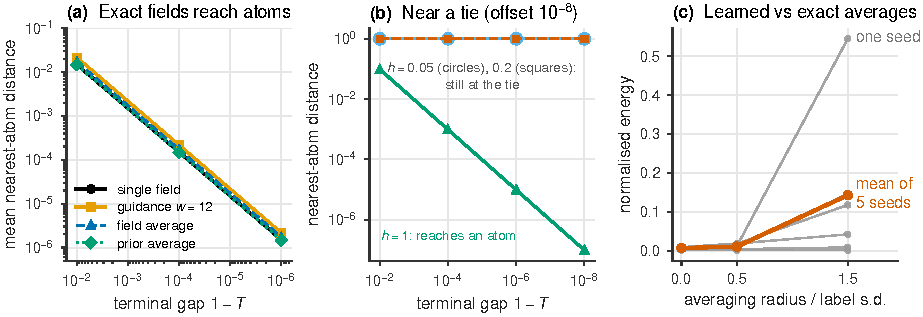
\includegraphics[width=0.98\textwidth]{fig_intervention_validation.pdf}
\caption{Intervention diagnostics. (a) Mean exact-field finite-cutoff distances for $d=2$,
random atoms, $h=1$, averaged over five geometry seeds. (b) Sources at offset $10^{-8}$ from
a symmetric tie under field averaging; delayed departure at a finite cutoff does not imply a
non-atom limit. (c) Learned versus exact field averages from five checkpoints: each seed (grey)
and their mean.}
\label{fig:intervention-validation}
\end{figure}
\placeblock{learnedtab}

\paragraph{Exact-field stress test.} Geometry seeds 201--205 generate $N=12$ atoms in dimensions
$2$ and $8$; the near-duplicate control moves the second atom to distance $0.02$ from the first.
For each $h\in\{0.3,1\}$ the arms are guidance at $w=0,3,12$, a uniform average of five fields at
label offsets $\{-2,-1,0,1,2\}h$, and the field of the average of their normalised priors. Each
cell uses 128 common Gaussian sources and double-precision log-time RK4 with 256 or 512 steps per
segment through the gaps $10^{-2},10^{-4},10^{-6}$. The 200 cells are nested within five geometry
seeds. \placeblock{stressextra}

\paragraph{Positive control.} \texttt{stress\_positive\_control.py} transcribes the oracle field and
the fixed-step RK4 of the stress test into double-precision NumPy and applies them to the guided
average of two conditional fields with log priors $(\mp B,\pm B)$ on the atoms $(-1,0)$ and
$(1,0)$, $B=1$, at $w/w_c\in\{0.9,1.1,2,10\}$, with $4096$ sources drawn from $\N(0,I_2)$ (seed
$20261121$). The second coordinate decays like $e^{-\tau}$, and the first follows the
one-dimensional composite of Theorem~\ref{thm:composition}, so the exact basin of the midpoint is
the interval of first coordinates found by bisection below. For each source the script compares the
fixed-step endpoint, called at the midpoint when it lies within $0.05$ of it, with membership of
the exact interval: there is no disagreement at any gap, step count or guidance strength. The
captured endpoints lie within $2.25\times10^{-17}$, $2.25\times10^{-19}$ and $2.25\times10^{-21}$ of
the midpoint along the line of the atoms, and within $0.0371$, $3.71\times10^{-4}$ and
$3.71\times10^{-6}$ across it, at the gaps $10^{-2}$, $10^{-4}$ and $10^{-6}$.


\paragraph{Ties.} In one dimension the atoms and labels are $\{-1,1\}$, with initial sources
$0,\pm10^{-12},\pm10^{-8},\pm10^{-4},\pm10^{-2}$ and $h\in\{0.05,0.2,1\}$. We compare the average of
the two exact label fields, the uniform-prior field, and the hard-label average, whose field is
$-x/(1-t)$ and whose endpoint is $0$. A follow-up to gap $10^{-18}$ shows departure toward the
atoms for positive offsets under fixed-step refinement, but DOP853 (relative tolerance $10^{-11}$,
absolute $10^{-30}$) fails in four of six selected cases at $h=0.05,0.2$ because the required
step falls below floating-point spacing; we retain these failures.
\placeblock{neartie}

\paragraph{Guided label averaging.} \texttt{composition\_counterexample.py} integrates $x$ with
Radau (relative tolerance $10^{-11}$, absolute $10^{-13}$) up to $\tau=0.5$ and then
$\dot s=\beta F(s)+(1+\eps/t)s$. Every $0.25$ units of $\tau$ it checks two stopping rules, each
forward invariant: $s$ beyond $\max(0,\text{largest root of }F)$ (limit $1$) or below
$\min(0,\text{smallest root})$ (limit $-1$); or $|s-s^\star|\le\delta$ around a root with
$F(s^\star-\delta)>0>F(s^\star+\delta)$ and $\beta\min\{F(s^\star-\delta),-F(s^\star+\delta)\}>
(1+\eps/t)(|s^\star|+\delta)$ (limit $0$). Roots are bracketed on a grid over $[-60,60]$ and refined
by Brent's method. The basin of $0$ is an interval located by bisection to relative tolerance
$10^{-12}$, and its probability is computed under $\N(0,1)$. Table~\ref{tab:composition} lists
the probabilities shown in Figure~\ref{fig:composition}(b).
\placeblock{compfig}
\placeblock{compperturb}

\placeblock{spectralexp}

\paragraph{Spectral criterion.} \texttt{spectral\_criterion\_check.py} draws Gaussian sources,
integrates $dx/d\tau=M(\beta x)-x$ with RK4 up to $t=1/2$, and then the exact profile equation
$d\xi/d\sigma=M(\xi)+\xi/(t\beta)$, $d\tau/d\sigma=1/\beta$ with an adaptive Runge--Kutta method
(relative tolerance $10^{-8}$) to $\sigma=10^4$. It records the fraction of sources with $|\xi|<5$
at $\sigma=10,10^2,10^3,10^4$; the fractions are unchanged from $\sigma=10^2$ on except for one box
source near its basin boundary. Table~\ref{tab:spectral} gives the results.
\texttt{theory\_basin\_map.py} integrates the triangle in the same two stages, with relative
tolerance $10^{-9}$, from $32768$ sources (seed $20261121$), and classifies the endpoint of every
source among all candidates at $\sigma=10^4$: the centre when $|\xi|<5$, an edge midpoint when the
trajectory lies within $0.2$ of it and its edge profile $\langle\xi,(a_i-a_j)/2\rangle$ is bounded
by $5$, and an atom when the trajectory lies within $0.2$ of it and every posterior puts weight
above $1-10^{-6}$ on it. At $1.1$, $2$, $5$ and $10\,w_c$ every source is classified, at $2$, $5$
and $10\,w_c$ no class changes after $\sigma=10^3$, and the centre fractions agree with
Table~\ref{tab:spectral} within sampling error. On the first $4096$ sources of
Table~\ref{tab:learned-composition} its centre classes coincide with those of
\texttt{learned\_composition\_2d.py}, whose classifier assigned each source ending at an edge
midpoint to one of that edge's atoms. With the configurations, sources (seed $11$) and integration
of \texttt{spectral\_criterion\_check.py}, \texttt{theory\_basin\_map.py} also classifies every
endpoint of Table~\ref{tab:spectral} by the face of atoms whose centroid it reaches: the atoms whose
weight under the uniform prior is within a factor $e^{50}$ of the largest, accepted when the
centroid has exactly these atoms as nearest atoms, the trajectory lies within $0.2$ of it and the
profile $\beta P_L(x-tz)$ on the span $L$ of the face is bounded by $5$. Every source is
classified, no class changes after $\sigma=10^3$ at $2$ and $5\,w_c$ or for the rectangle and the
box, and the centre fractions equal those of Table~\ref{tab:spectral} for the rectangle and the box
and agree within sampling error for the triangle and the simplex, whose atoms come from a singular
value decomposition that linear-algebra libraries may return rotated.

\begin{table}[htb]
\centering\small
\begin{tabular}{@{}lrrlcrrrr@{}}
\toprule
configuration & $d$ & $N$ & $w$ & profile $\xi=0$ & $\tr\Gamma$ & sources & $\sigma=10^2$ & $\sigma=10^4$\\
\midrule
triangle & 2 & 3 & $0.5\,w_c$ & source & $0.268$ & 2048 & $0.0000$ & $0.0000$\\
triangle & 2 & 3 & $0.9\,w_c$ & source & $0.054$ & 2048 & $0.0000$ & $0.0000$\\
triangle & 2 & 3 & $1.1\,w_c$ & sink & $-0.054$ & 2048 & $0.0010$ & $0.0010$\\
triangle & 2 & 3 & $2\,w_c$ & sink & $-0.537$ & 2048 & $0.1396$ & $0.1396$\\
triangle & 2 & 3 & $5\,w_c$ & sink & $-2.148$ & 2048 & $0.6865$ & $0.6865$\\
simplex & 8 & 9 & $0.5\,w_c$ & source & $0.414$ & 2048 & $0.0000$ & $0.0000$\\
simplex & 8 & 9 & $0.9\,w_c$ & source & $0.083$ & 2048 & $0.0000$ & $0.0000$\\
simplex & 8 & 9 & $1.1\,w_c$ & sink & $-0.083$ & 2048 & $0.0000$ & $0.0000$\\
simplex & 8 & 9 & $2\,w_c$ & sink & $-0.828$ & 2048 & $0.0000$ & $0.0000$\\
simplex & 8 & 9 & $5\,w_c$ & sink & $-3.311$ & 2048 & $0.0186$ & $0.0186$\\
rectangle & 2 & 4 & $1$ & saddle & $-0.572$ & 2048 & $0.0000$ & $0.0000$\\
rectangle & 2 & 4 & $5$ & sink & $-3.717$ & 2048 & $0.2461$ & $0.2461$\\
box & 8 & 256 & $1$ & saddle & $-0.572$ & 512 & $0.0000$ & $0.0000$\\
box & 8 & 256 & $5$ & sink & $-3.717$ & 512 & $0.0039$ & $0.0020$\\
\bottomrule
\end{tabular}
\caption{Numerical check of Theorem~\ref{thm:spectral}: fraction of Gaussian sources whose
profile $\xi$ stays in $\{|\xi|<5\}$ at fast time $\sigma$, an estimate of $\Pr(X_1=z)$ for $z=0$.
The class of the profile and $\tr\Gamma$ are computed from $\Gamma(0)$. For the triangle and the
simplex, $w_c=(1-m^2)/m^2$ is the threshold of Corollary~\ref{cor:spectral-threshold}
($1.160$ and $4.802$ at $B=2$). The rectangle and the box at $w=1$ are saddles with negative
trace. Other candidates are not counted: on the triangle the edge midpoints, ties of two atoms
whose profile attracts for $w>1.368\,w_c$, take a further $0.41$ and $0.29$ of the mass at $2$ and
$5\,w_c$; on the simplex at $2$ and $5\,w_c$ and on the rectangle and the box, centroids of other
faces take most of the mass (\ificlr Appendix~\ref{app:intervention-protocol}\else
Section~\ref{sec:intervention-tests}\fi).}
\label{tab:spectral}
\end{table}

\begin{table}[h]
\centering\small
\begin{tabular}{@{}lrrrrrrr@{}}
\toprule
& & \multicolumn{4}{c}{$w/w_c$} & \multicolumn{2}{c}{$w$}\\
\cmidrule(lr){3-6}\cmidrule(l){7-8}
$B$ & $w_c$ & $\le0.9$ & $1.1$ & $2$ & $10$ & $1$ & $3$\\
\midrule
1 & 0.7241 & 0 & 0.050 & 0.406 & 0.991 & 0.179 & 0.808\\
2 & 0.0760 & 0 & 0.021 & 0.182 & 0.809 & 0.891 & 0.999\\
3 & 0.0100 & 0 & 0.008 & 0.069 & 0.396 & 0.987 & $>0.999$\\
\bottomrule
\end{tabular}
\caption{Probability under $\pi_0$ that the guided label average of
Theorem~\ref{thm:composition} ends at the non-training midpoint $0$, with threshold
$w_c=1/\sinh^2B$. The entry $0$ (at $w/w_c\in\{0.5,0.9\}$) means that only the source $x_0=0$
reaches the midpoint, as Theorem~\ref{thm:composition}(b) states; the other entries are
floating-point exact-flow computations with stopping criteria justified by the proof, and
bisection; they are not verified by interval arithmetic.}
\label{tab:composition}
\end{table}

\paragraph{Learned guided label averaging.}
\label{app:learned-composition}
\texttt{learned\_composition.py} trains on $\D=\{(-1,-1),(1,1)\}$ with Gaussian label noise
$h=1$, and \texttt{learned\_composition\_2d.py} on three atoms on the unit circle with one-hot
labels and $h=1$. Every network is an MLP of width $128$ and depth $4$, trained for $2\times10^5$
steps with batch $2048$, AdamW without weight decay, learning rate $3\times10^{-3}$ (the lowest
held-out CFM loss among $\{3\times10^{-4},10^{-3},3\times10^{-3}\}$ at $5\times10^4$ steps, one
seed), a cosine schedule, gradient clipping at~$1$ and condition dropout $0.1$, with fresh
interpolant samples at every step. The velocity network regresses $X_1-X_0$; its log-uniform
variant draws $1-t$ half uniformly and half log-uniformly on $[10^{-5},1]$ with importance weights,
so that the objective is unchanged, and its separate-unconditional variant (four seeds) replaces
dropout by a second network. The data-predicting network regresses $X_1$ with input
$\operatorname{asinh}(tx/(1-t)^2)$ in addition to $(x,t,y)$. The distillation network has the same
architecture but regresses the exact posterior mean at interpolant samples and at points of the
boundary layer; it is a positive control for the solver and the architecture at the tie where its
input is centred (on the triangle it also leaves the edge midpoints empty), not a model learned from
data. Composites are integrated from the first $2048$ of $16384$ shared Gaussian
sources in $\tau=-\log(1-t)$, first in $x$ and then in $s=tx/(1-t)^2$, by a per-source adaptive
Rosenbrock method (ROS2) at relative tolerances $10^{-5}$ and $10^{-7}$. Occupancy is
the fraction of sources within $\delta$ of the midpoint at the gap $\epsilon=1-t$, reported at
$\epsilon=10^{-5}$, $\delta=0.05$; the radii $0.02$ and $0.1$ are in the artifacts. Over every
network, seed and guidance strength of Table~\ref{tab:learned-composition} and
Appendix~\ref{apx:bottleneck-runs} (\texttt{summarize\_composite\_solver\_checks.py}), the endpoint
classes of the composite differ between the two tolerances for at most $1.32\%$ of the sources in
the two-atom runs ($B=1,2,3$) and $0.98\%$ on the triangle, and the occupancy changes by at most
$0.005$ and $0.009$. The exception is the off-tie network of Appendix~\ref{apx:bottleneck-runs} at
$w\ge2w_c$, whose classes differ for up to $53\%$ of the sources (one seed, $5w_c$) while its
occupancy stays below $0.011$ at both tolerances. Between $\epsilon=10^{-3}$ and $10^{-5}$ the
occupancy changes by at most $0.020$ in the two-atom runs, except at $B=3$, where the velocity
networks fail anyway (up to $0.049$), and by at most $0.055$ on the triangle, where it is still
rising in one data-predicting seed at $5w_c$ ($0.680$ to $0.735$). A fixed-step RK4
in~$\tau$, used first, is unstable once $\beta|F'|\,\Delta\tau>2.8$ and ejects the trajectories
an attracting tie holds; it gave no midpoint mass even for the positive control, and we discarded
it. The exact one-dimensional probabilities are computed as for Table~\ref{tab:composition}
(\texttt{learned\_composition\_exact.py}) and agree with its entries; on the
triangle the exact value is the fraction of the first $4096$ sources whose profile stays bounded,
$|\xi|<5$, under the profile integration of Table~\ref{tab:spectral}, that is, the fraction ending
at the centre; sources ending at an edge midpoint were assigned to one of that edge's atoms, which
leaves this fraction unchanged. \texttt{theory\_basin\_map.py} counts the learned endpoints within
$0.05$ of an edge midpoint, and those farther than $0.1$ from every atom and from the centre, in the
stored final states of the standard, the data-predicting and the distillation networks on the
triangle (Section~\ref{sec:intervention-tests}). At $B=3$, where $w_c=0.010$, the velocity networks place
mass at the midpoint at every $w$, including $w=0$, where the exact field places none, with seed
standard deviations as large as the means: an error of the learned field, not a basin of the
exact one. The label average alone, single-label guidance and guided prior averaging, whose
exact endpoints are atoms almost surely, keep the learned two-atom midpoint occupancy at most
$0.001$, except for the label average of the velocity networks at $B=3$ and of the velocity network
with the rescaled input at $B=2$ ($0.009\pm0.018$, Table~\ref{tab:learned-composition}). The data-predicting network starts slightly
early ($0.014\pm0.009$ at $w=w_c$, $B=1$): its fitted tie slope changes sign at about $0.87\,w_c$
near $t=1$. \placeblock{lossrisk}

\paragraph{Which change matters.} Two ablations separate the changes, with five seeds each and
the same training and integration. \texttt{cfm\_v\_s} keeps the velocity output and its loss and
adds only the input $\operatorname{asinh}(tx/(1-t)^2)$; \texttt{cfm\_x} predicts the data with the
data loss and has no extra input (rows ``rescaled input'' and ``data, plain input'' of
Table~\ref{tab:learned-composition}). With the input, a velocity network reproduces the exact
probabilities when it succeeds, but not in every seed: at $B=1$ all five seeds give
$0.877$--$0.885$ at $5w_c$ and four give $0.299$--$0.406$ at $2w_c$ while one gives $0$; at $B=2$
four seeds match at $10w_c$ and two at $5w_c$; at $B=3$ it fails as the velocity network does.
On the triangle four of five seeds match the exact probabilities at the centre ($0.687$--$0.735$ against
$0.673$ at $5w_c$, $0.948$--$0.971$ against $0.952$ at $10w_c$) and one fails
($0.055$ and $0.013$).
Without the input, the data-predicting network places less than $0.001$ of its sources at the
midpoint at $w\ge5w_c$ for every $B$ and seed, and none at any $w$ on the triangle; at $B=1$ and $2w_c$ one seed places $0.415$ and the
others none. Its endpoints are then fixed points of its prediction at $t=1$, which
Proposition~\ref{prop:regular}(b) describes for a bounded prediction, although the trained network
is not clipped. In these runs the rescaled input is necessary, and the data parametrisation makes
it reliable across seeds at $B=1,2$ and on the triangle; at $B=3$ one of five seeds places no source
at the midpoint at $2$ and $5\,w_c$.

\paragraph{Tie-centring and a label bottleneck.}
\label{apx:bottleneck-runs}
On the triangle, further data-predicting networks, three seeds each, use the loss and training of
the rescaled-input network (\texttt{server\_bottleneck\_2d\_cpu.sh}). \texttt{cfm\_x\_o} receives the
rescaled input centred at $(0.3,0.2)$ instead of the tie $z=0$. Its label average places no source
at the midpoint at any guidance strength in any seed, against $0.133$ for the exact field at $2w_c$
and $0.952$ at $10w_c$, and at $w\le2w_c$ at least $0.96$ of its sources end within $0.05$ of an
atom. In these runs the composition is learned only by a network told where the tie is, and only
at that tie: the data-predicting network told the centre leaves the edge midpoints empty
(Section~\ref{sec:intervention-tests}). A
variant with one rescaled input centred at each vertex (\texttt{cfm\_x\_a}) could not be
evaluated: its learned composite is so stiff that the two solver tolerances disagree on the
endpoint class of $4\%$ and $27\%$ of the sources already at $w=0$, and in one seed the tight solver
did not finish; we stopped these runs.

\texttt{cfm\_x\_sq} sees its noised label only through the cell $\arg\max_k y_k$, a bottleneck as in
Proposition~\ref{prop:bottleneck}. The cell priors favour their vertex with $B_Q=1.2413$, so
$w_c(B_Q)=3.926$, and its guidance strengths are in units of $w_c(B_Q)$. Averaging its field over
labels averages the three cell fields, and the learned composite follows the exact composite of
those fields at the centre at $5$ and $10\,w_c(B_Q)$, though not in every seed at $2w_c(B_Q)$ (its
edge midpoints, which attract for $w>1.001\,w_c(B_Q)$, are not counted): $0.718$, $0.817$ and
$0.747$ against $0.757$ at $5w_c(B_Q)$, $0.983$ to $0.989$ against $0.972$ at $10w_c(B_Q)$, and
$0.135$, $0.226$ and $0$ against $0.179$ at $2w_c(B_Q)$. Single-label
guidance places no source at the midpoint at $w\le2w_c(B_Q)$ in any seed, as
Proposition~\ref{prop:bottleneck}(b) states for the exact field, but only $0.14$ to $0.64$ of the
sources end within $0.05$ of an atom at $2w_c(B_Q)$. At $10w_c(B_Q)\approx39$, where guidance
amplifies the learning error most, one seed places $0.92$ of its sources at the midpoint and the
other two end at neither the atoms nor the midpoint (at most $0.013$ at an atom). These are errors
of the learned field, whose exact endpoints are atoms almost surely.

\paragraph{Guided label averaging on CIFAR-10.}
\label{app:cifar-composition}
\texttt{cifar\_composition\_exact.py} applies the composite of Theorem~\ref{thm:composition} to the
CIFAR-10 inpainting problem ($N=2000$ training images in $\R^{3072}$, labels their top
halves, $k=1536$), averaging the exact conditional fields at the labels $y^i,y^j$ of a pair and guiding
against the unconditional one. The label bandwidth is set to $h=|y^i-y^j|/2$, so that $B=1$ and
$w_c=0.724$. We use eight pairs whose midpoint $z=(x^i+x^j)/2$ is farther than
$\sqrt{5.2}\,r$, $r=|x^i-x^j|/2$, from every other training image, and $512$ shared Gaussian
sources. Of the $81$ mutual-nearest-neighbour pairs among the $2000$ images, all have no other
image within $r$ of their midpoint, as Theorem~\ref{thm:spectral}(c) requires, and these eight
are the ones with the largest margin. Their images lie at $0.54$ to $0.90$ times the median
nearest-neighbour distance of the $2000$ images: similar but distinct images
(Figure~\ref{fig:cifar-composition}a). So that the selection does not decide the result, we also
ran twelve of the other $73$ pairs, drawn at random (seed $20261108$,
\texttt{cifar\_mutual\_pairs.py}), at $w/w_c\in\{0.9,1.1,2,5\}$; every one of the $81$ pairs has
margin at least $3.2$. In them no source ends at the midpoint at $0.9w_c$; at $1.1w_c$ ten of the
twelve have some ($0.002$ to $0.014$) and two have none of their $512$ sources; at $2w_c$ all
have some ($0.006$ to $0.088$, mean $0.042$), and at $5w_c$ the mean is $0.038$. At most one
source in a pair is unresolved. These basins are smaller than in the selected pairs, in line
with the trend in the margin below. Each trajectory of the full $2000$-atom field is integrated with an adaptive
Bogacki--Shampine method (relative tolerance $10^{-6}$) until all three posteriors put all but
$10^{-12}$ of their mass on the pair, where the flow along $x^i-x^j$ is exactly the
one-dimensional flow of Theorem~\ref{thm:composition} and is finished with Radau and classified by
the roots of $F_w$, or on one atom, which is then the endpoint; no source remained unresolved.
The classifier returns the midpoint only when $w>w_c$ and $|s|<s_u$, with $\pm s_u$ the outer roots
of $F_w$, so the zero midpoint fractions reported here for $w\le0.9w_c$ follow from
Theorem~\ref{thm:composition}(b) and do not test it.
For $w/w_c\in\{0,0.5,0.9\}$ no source in any pair ends at the midpoint. At $w/w_c=1.1$ every
pair has some ($0.006$ to $0.043$, mean $0.025$), and the fraction peaks at $w/w_c=2$ ($0.027$ to
$0.291$, mean $0.186$) before falling at $5$ (mean $0.150$) and $10$ (mean $0.042$), as guidance
pulls more sources onto the pair's atoms; the fraction ending on the pair or its midpoint grows
from $0.06$--$0.96$ at $w=0$ to $0.58$--$1$ at $w=10w_c$. Pairs whose midpoint is farther from
the other images tend to have larger midpoint fractions. We reran all eight pairs at
$w/w_c\in\{0.9,1.1,2\}$ with a hand-off at $10^{-9}$ and, separately, a relative tolerance of
$10^{-8}$. No source ends at the midpoint at $0.9w_c$ in any pair or setting. At $1.1w_c$ every
pair stays positive in all three settings, from $0.006$ ($3$ of $512$ sources, in two pairs, the
same in every setting) to $0.047$, and the three settings differ by at most $0.006$ in any pair;
at $2w_c$ they differ by at most $0.018$. Individual endpoints agree with the main run for at
least $99\%$ of sources at $1.1w_c$ and $87\%$ at $2w_c$. We reran all eight pairs at $5w_c$ and
$10w_c$ in the same two settings (\texttt{cifar\_composition\_random\_20261108}): there individual
endpoints agree with the main run for only $41\%$ to $92\%$ of the sources, and the class
(midpoint, an atom of the pair, another atom) for $66\%$ to $98\%$, so we report fractions only.
The midpoint fraction of a pair changes by at most $0.064$ at $5w_c$ and $0.029$ at $10w_c$, and
its mean over the pairs is $0.139$ to $0.150$ at $5w_c$ and $0.040$ to $0.042$ at $10w_c$ across
the three settings, so its fall after $2w_c$ is not a solver effect. The midpoints are blends of two training images, not
training images. The threshold itself is not new evidence: the midpoint of each pair is a
candidate whose only nearest atoms are $x^i,x^j$, all priors are positive, and
Theorem~\ref{thm:spectral}(c) with the two-atom computation of Corollary~\ref{cor:spectral-threshold}
gives $\Pr(X_1=z)>0$ exactly when $w>w_c$. The computation is a consistency check of that
prediction at $d=3072$ with the other $1998$ atoms present, and it measures the basin sizes,
which the theorem does not give. Outputs are under \texttt{results/\iclrallow cifar\_composition\_exact\_20261105/};
\texttt{make\_theory\_cifar\_composition\_figure.py} draws Figure~\ref{fig:cifar-composition}.

\begin{figure}[htb]
\centering
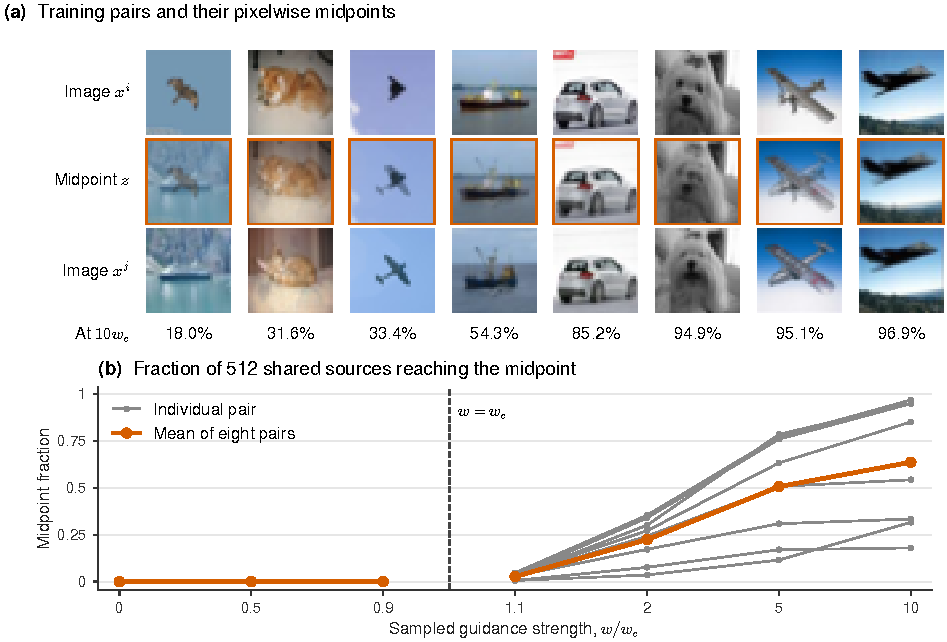
\includegraphics[width=\textwidth]{fig_cifar_composition.pdf}
\caption{Exact guided label averaging on CIFAR-10 ($N=2000$, $d=3072$, $B=1$). (a) Three of the
eight pairs: the training images $x^i,x^j$ and the midpoint $z$ (framed), which the composite
reaches with positive probability for $w>w_c$. (b) Fraction of $512$ shared sources ending at $z$
for each pair (thin) and the mean over pairs (thick); it is zero for $w\le0.9w_c$, where the
classifier excludes the midpoint (Theorem~\ref{thm:composition}(b)), and $w=0$ is drawn left of the
axis break.}
\label{fig:cifar-composition}
\end{figure}

\begin{table}[htb]
\centering\footnotesize\setlength{\tabcolsep}{3.5pt}
\newcommand{\lctable}{%
\begin{tabular}{@{}llrrrrrr@{}}
\toprule
& & \multicolumn{6}{c}{$w/w_c$}\\
\cmidrule(l){3-8}
& network & $0$ & $1$ & $1.1$ & $2$ & $5$ & $10$\\
\midrule
$B=1$ & exact & $0.000$ & $0.000$ & $0.050$ & $0.406$ & $0.878$ & $0.991$\\
 & velocity CFM & $0.000\pm0.000$ & $0.000\pm0.000$ & $0.000\pm0.000$ & $0.000\pm0.000$ & $0.000\pm0.000$ & $0.000\pm0.000$\\
 & \quad log-uniform $1-t$ & $0.000\pm0.000$ & $0.000\pm0.000$ & $0.000\pm0.000$ & $0.000\pm0.000$ & $0.000\pm0.000$ & $0.000\pm0.000$\\
 & \quad separate unconditional & $0.000\pm0.000$ & $0.000\pm0.000$ & $0.000\pm0.000$ & $0.000\pm0.000$ & $0.000\pm0.000$ & $0.000\pm0.000$\\
 & \quad rescaled input & $0.000\pm0.000$ & $0.012\pm0.014$ & $0.023\pm0.026$ & $0.294\pm0.152$ & $0.881\pm0.003$ & $0.991\pm0.000$\\
 & data, plain input & $0.000\pm0.000$ & $0.001\pm0.003$ & $0.003\pm0.005$ & $0.083\pm0.166$ & $0.000\pm0.000$ & $0.000\pm0.000$\\
 & data, rescaled input & $0.000\pm0.000$ & $0.014\pm0.009$ & $0.054\pm0.004$ & $0.401\pm0.006$ & $0.878\pm0.001$ & $0.991\pm0.000$\\
 & distillation (control) & $0.000\pm0.000$ & $0.000\pm0.000$ & $0.049\pm0.000$ & $0.407\pm0.000$ & $0.878\pm0.000$ & $0.991\pm0.000$\\
\midrule
$B=2$ & exact & $0.000$ & $0.000$ & $0.021$ & $0.182$ & $0.532$ & $0.809$\\
 & velocity CFM & $0.001\pm0.001$ & $0.001\pm0.002$ & $0.001\pm0.002$ & $0.001\pm0.001$ & $0.001\pm0.001$ & $0.000\pm0.000$\\
 & \quad log-uniform $1-t$ & $0.000\pm0.000$ & $0.000\pm0.000$ & $0.000\pm0.000$ & $0.000\pm0.000$ & $0.000\pm0.000$ & $0.000\pm0.000$\\
 & \quad separate unconditional & $0.000\pm0.000$ & $0.004\pm0.006$ & $0.002\pm0.003$ & $0.002\pm0.003$ & $0.000\pm0.001$ & $0.000\pm0.000$\\
 & \quad rescaled input & $0.009\pm0.018$ & $0.019\pm0.035$ & $0.021\pm0.038$ & $0.038\pm0.066$ & $0.212\pm0.259$ & $0.646\pm0.323$\\
 & data, plain input & $0.000\pm0.001$ & $0.000\pm0.000$ & $0.000\pm0.000$ & $0.000\pm0.000$ & $0.000\pm0.000$ & $0.000\pm0.000$\\
 & data, rescaled input & $0.000\pm0.000$ & $0.004\pm0.007$ & $0.020\pm0.015$ & $0.177\pm0.007$ & $0.530\pm0.004$ & $0.808\pm0.003$\\
 & distillation (control) & $0.000\pm0.000$ & $0.000\pm0.000$ & $0.018\pm0.001$ & $0.179\pm0.000$ & $0.535\pm0.000$ & $0.809\pm0.000$\\
\midrule
$B=3$ & exact & $0.000$ & $0.000$ & $0.008$ & $0.069$ & $0.221$ & $0.396$\\
 & velocity CFM & $0.048\pm0.083$ & $0.048\pm0.086$ & $0.048\pm0.086$ & $0.049\pm0.088$ & $0.051\pm0.094$ & $0.056\pm0.104$\\
 & \quad log-uniform $1-t$ & $0.023\pm0.045$ & $0.023\pm0.046$ & $0.022\pm0.045$ & $0.020\pm0.040$ & $0.009\pm0.019$ & $0.001\pm0.001$\\
 & \quad separate unconditional & $0.081\pm0.137$ & $0.085\pm0.147$ & $0.085\pm0.147$ & $0.090\pm0.154$ & $0.105\pm0.181$ & $0.126\pm0.219$\\
 & \quad rescaled input & $0.034\pm0.067$ & $0.036\pm0.072$ & $0.037\pm0.073$ & $0.038\pm0.076$ & $0.044\pm0.087$ & $0.061\pm0.121$\\
 & data, plain input & $0.000\pm0.000$ & $0.000\pm0.000$ & $0.000\pm0.000$ & $0.000\pm0.000$ & $0.000\pm0.000$ & $0.000\pm0.000$\\
 & data, rescaled input & $0.000\pm0.000$ & $0.010\pm0.013$ & $0.013\pm0.016$ & $0.056\pm0.030$ & $0.167\pm0.084$ & $0.378\pm0.009$\\
 & distillation (control) & $0.000\pm0.000$ & $0.000\pm0.000$ & $0.008\pm0.000$ & $0.066\pm0.000$ & $0.217\pm0.000$ & $0.395\pm0.000$\\
\midrule
triangle & exact & $0.000$ & -- & $0.002$ & $0.133$ & $0.673$ & $0.952$\\
 & velocity CFM & $0.000\pm0.000$ & -- & $0.000\pm0.000$ & $0.000\pm0.000$ & $0.000\pm0.000$ & $0.000\pm0.000$\\
 & \quad rescaled input & $0.000\pm0.000$ & -- & $0.015\pm0.011$ & $0.146\pm0.077$ & $0.579\pm0.262$ & $0.769\pm0.378$\\
 & data, plain input & $0.000\pm0.000$ & -- & $0.000\pm0.000$ & $0.000\pm0.000$ & $0.000\pm0.000$ & $0.000\pm0.000$\\
 & data, rescaled input & $0.000\pm0.000$ & -- & $0.001\pm0.002$ & $0.143\pm0.004$ & $0.692\pm0.023$ & $0.962\pm0.005$\\
 & distillation (control) & $0.002\pm0.005$ & -- & $0.007\pm0.011$ & $0.140\pm0.004$ & $0.699\pm0.037$ & $0.961\pm0.012$\\
\bottomrule
\end{tabular}}
\ificlr\resizebox{\textwidth}{!}{\lctable}\else\lctable\fi
\caption{Midpoint occupancy of learned guided label averages, mean $\pm$ population standard
deviation over seeds, at $\epsilon=10^{-5}$, $\delta=0.05$, from $2048$ shared sources; exact
rows give the exact probability of the midpoint (computed as for Table~\ref{tab:composition} by
\texttt{learned\_composition\_exact.py}; triangle: fraction
of the first $4096$ sources ending at the centre, $0.138$, $0.681$ and $0.951$ on the $2048$
sources of the networks at $2$, $5$ and $10\,w_c$). The exact triangle composite ends a further
$0.426$, $0.306$ and $0.048$ of these $4096$ sources at the edge midpoints, which the occupancies
do not count (Section~\ref{sec:intervention-tests}). The triangle grid has no $w=w_c$.}
\label{tab:learned-composition}
\end{table}

\FloatBarrier
\placeblock{learnedpilot}

\paragraph{Learned label averages.} The five networks have problem seeds 1001--1005, $h=0.1$ and
$2\times10^5$ training steps. For each, the first and last training labels and two fresh queries
are evaluated at three radii $r/\operatorname{sd}(y)\in\{0,0.5,1.5\}$, giving 60 model--query cells.
The network keeps its float32 time embedding and uses original-time RK4 with 400/800 steps to
$T=0.999$; the exact average uses double-precision log-time RK4 with 768/1536 steps to the same
cutoff. The normalised biased energy V-statistic uses 128 generated and reference samples,
averaged over queries within each seed and then over seeds. At fresh queries the mean
nearest-atom distances are $0.0573$, $0.0916$, $0.1106$ for the network and $0.00183$,
$0.00328$, $0.00479$ for the exact average.

\begingroup\raggedright
\paragraph{Artifacts.} Raw arrays and per-cell outputs are under
\texttt{results/\iclrallow novelty\_interventions\_20261016/} and
\texttt{results/\iclrallow theory\_composition\_20261019/}, the positive control under
\texttt{results/\iclrallow stress\_positive\_control\_20261121/}; the endpoint laws on the triangle of
Figure~\ref{fig:unrolled} and Section~\ref{sec:intervention-tests}, the face masses of the
configurations of Table~\ref{tab:spectral} and the learned edge counts are under
\texttt{results/\iclrallow theory\_basin\_map\_20261121/}; the learned composition is under
\texttt{results/\iclrallow learned\_composition\_20261021/} and
\texttt{results/\iclrallow learned\_composition\_2d\_20261021/}, with
Figure~\ref{fig:learned-composition} and Table~\ref{tab:learned-composition} drawn by
\texttt{make\_learned\_composition\_figure.py}. An independent recomputation checked all 984
primary metric rows and 84 refinement rows of the stress and tie tests.\par\endgroup

\end{document}
